\clearpage

\phantomsection

\setcounter{chapter}{0}
\chapter[{CƠ SỞ LÝ THUYẾT VÀ TỔNG QUAN NGHIÊN CỨU}]{CƠ SỞ LÝ THUYẾT VÀ TỔNG QUAN NGHIÊN CỨU}

\section{Mạng Nơ-ron Tích chập}

Mạng Nơ-ron Tích chập (Convolutional Neural Networks – CNNs) đã củng cố vị thế
là kiến trúc nền tảng trong lĩnh vực thị giác máy tính, tạo ra những bước tiến lớn trong 
các tác vụ từ phân loại ảnh đơn giản đến phân đoạn thực thể phức tạp. Sự thành công của CNN bắt 
nguồn từ khả năng học hỏi các biểu diễn đặc trưng phân cấp, tự động trích xuất các thông tin hình 
học ngày càng trừu tượng từ dữ liệu đầu vào thô. \cite{Basha2020} 
\begin{figure}[H]
    \centering
    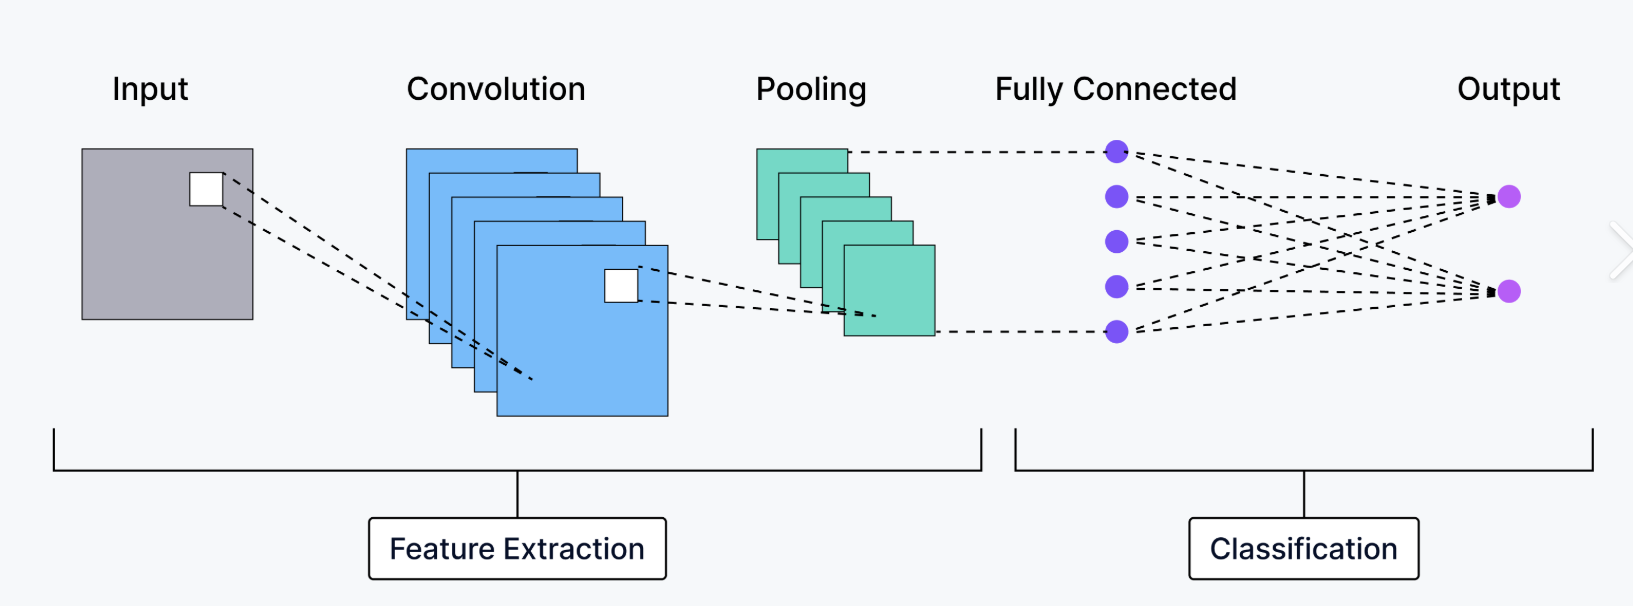
\includegraphics[width=0.8\textwidth]{figChap1/CNN_kien_truc.png}
    \caption{Mạng Nơ-ron Tích chập cơ bản}
    \label{fig:convolutional_neural_network}
\end{figure}

\subsection{Hoạt động của Lớp Tích chập}

Lớp tích chập là khối xây dựng cơ bản của mọi kiến trúc CNN hiện đại. Cơ chế hoạt động của lớp này được 
thiết kế đặc biệt để xử lý dữ liệu ảnh bằng cách khai thác tính cục bộ và tính bất biến dịch chuyển 
thống kê của đặc trưng hình ảnh.

Lớp tích chập vận hành thông qua các kernel nhỏ (hay còn gọi là bộ lọc). 
Các kernel này trượt (slide) trên ảnh đầu vào, thực hiện phép nhân tích chập với từng phần của 
ảnh để tính toán tích vô hướng cục bộ. Điều này cho phép lớp tích chập hoạt động như các bộ lọc 
cục bộ, chuyên trách trích xuất các đặc trưng hình học cơ bản, chẳng hạn như các cạnh (edges), 
đường cong (curves), hoặc các kết cấu (textures).\cite{Girshick2014}

Mỗi kernel trong lớp tích chập được học để phát hiện một loại đặc trưng cụ thể và áp dụng phát hiện 
đó trên toàn bộ ảnh. Khả năng học các bộ lọc cục bộ này, thay vì dựa vào các đặc trưng được thiết kế 
thủ công (handcrafted features) như SIFT hay HOG trong các mô hình thị giác máy tính truyền thống, 
là một đổi mới cốt lõi của CNN. Sự thay đổi này đã giúp các mô hình CNN giảm đáng kể nhu cầu về kinh 
nghiệm chuyên môn trong việc tiền xử lý dữ liệu đầu vào.\cite{Basha2020} Quá trình này tạo tiền đề cho việc xây dựng 
các đặc trưng phân cấp phong phú (rich hierarchy of image features), nơi các lớp sâu hơn dần dần 
kết hợp các đặc trưng cấp thấp thành các biểu diễn trừu tượng và ngữ nghĩa hơn.\cite{Girshick2014}

\subsection{Lớp Pooling và Tối ưu hóa Bản đồ Đặc trưng}

Thông thường, lớp Pooling được thêm vào ngay sau một lớp tích chập. Chức năng chính của lớp Pooling 
là giảm độ phân giải không gian của bản đồ đặc trưng (feature maps) bằng cách chia chúng thành các 
vùng con hình chữ nhật và giảm mẫu các đặc trưng trong mỗi vùng con thành một giá trị duy nhất, 
thường là giá trị trung bình (average) hoặc giá trị cực đại (maximum). \cite{WikiCNN}
\begin{figure}[H]
    \centering
    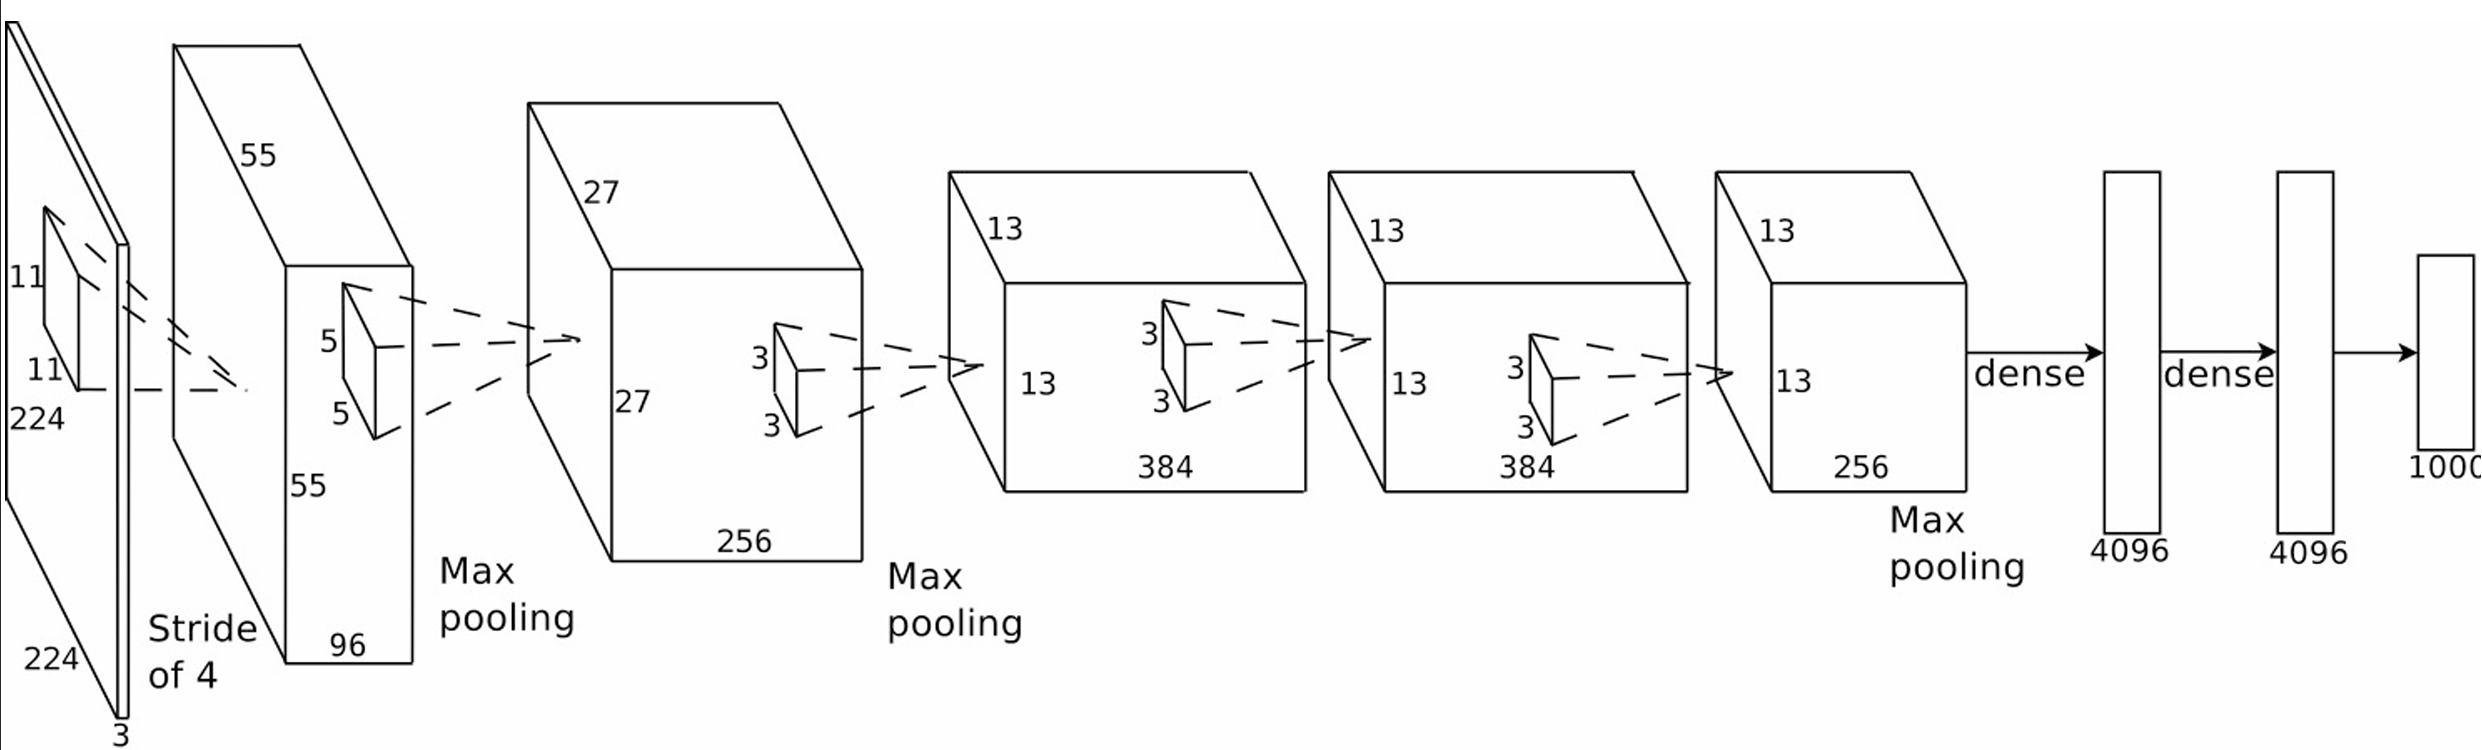
\includegraphics[width=0.8\textwidth]{figChap1/maxPooling.png}
    \caption{Lớp Pooling}
    \label{fig:pooling}
\end{figure}

Quá trình giảm mẫu này thực hiện hai mục đích quan trọng. Thứ nhất, nó giảm kích thước dữ liệu, 
làm giảm chi phí tính toán trong các lớp sau. Thứ hai, và quan trọng hơn về mặt lý thuyết, hoạt động 
pooling mang lại một mức độ bất biến dịch chuyển cục bộ (local translational invariance) cho các đặc 
trưng. Tính bất biến này giúp CNN trở nên vững vàng hơn (robust) đối với các biến thể nhỏ trong vị 
trí hoặc biến dạng của các đặc trưng, cho phép mô hình nhận dạng các đối tượng ngay cả khi chúng hơi 
bị dịch chuyển trong ảnh.\cite{WikiCNN}

Tuy nhiên, việc giảm độ phân giải không gian thông qua pooling là một sự đánh đổi. 
Mặc dù pooling tạo ra tính bất biến, nó cũng dẫn đến sự mất mát thông tin vị trí chính xác 
(spatial location). Sự mất mát này không đáng kể trong các tác vụ phân loại hình ảnh cấp độ toàn cục, 
nhưng lại trở thành một rào cản kỹ thuật nghiêm trọng đối với các tác vụ định vị mật độ cao 
(dense prediction tasks) như phân đoạn thực thể, đòi hỏi sự căn chỉnh pixel-to-pixel.\cite{He2017}

\subsection{Lớp Kết nối Đầy đủ và Phân loại Quyết định}

Các lớp tích chập và pooling hoạt động như các khối trích xuất đặc trưng (feature extractors). 
Để hoàn thành tác vụ phân loại, CNN cần các lớp kết nối đầy đủ (FC layers) ở phần cuối của kiến trúc. \cite{Basha2020}

Trước khi đi vào lớp FC, bản đồ đặc trưng 2D/3D cuối cùng được làm phẳng (flattened) thành một vector 1D.
Lớp FC là lớp cuối cùng của mạng, có chức năng tổng hợp toàn bộ các đặc trưng trừu tượng 
đã được trích xuất bởi các khối xử lý trước đó. Mỗi nơ-ron trong lớp FC này được 
kết nối với tất cả các đầu vào của lớp trước, và cuối cùng, lớp này gán một giá trị xác suất cho 
hình ảnh thuộc về từng lớp trong số $C$ lớp khả dĩ. \cite{Basha2020}

Một phát hiện quan trọng từ các nghiên cứu gần đây là mối quan hệ giữa độ sâu kiến trúc CNN và nhu cầu thiết kế 
lớp FC. Phân tích cho thấy:
Mạng Nông (Shallow CNNs), do các đặc trưng được trích xuất ở lớp tích chập cuối cùng ít trừu tượng hơn, 
mạng nông cần một số lượng lớn nơ-ron và nhiều lớp FC hơn để đạt được hiệu suất phân loại tương đương.
Mạng Sâu (Deeper CNNs), ngược lại, mạng sâu đã trích xuất được các đặc trưng trừu tượng hóa cao hơn. 
Do đó, chúng cần ít nơ-ron FC hơn để tổng hợp thông tin và đưa ra quyết định.
Việc hình thức hóa mối quan hệ này giữa kiến trúc và tập dữ liệu là một bước tiến quan trọng giúp
các nhà thực hành chuyển quá trình lựa chọn kiến trúc từ kinh nghiệm (expertise) sang một quy trình 
thiết kế tự động và có hệ thống. \cite{Basha2020}

\subsection{Các Hàm kích hoạt}

Hàm kích hoạt (Activation Function) là thành phần không thể thiếu trong Mạng Nơ-ron Tích chập, giúp mô hình giải quyết và biểu diễn các đặc trưng phi tuyến tính phức tạp có trong dữ liệu hình ảnh. Có rất nhiều hàm kích hoạt được sử dụng trong thực tế:
\begin{itemize}
    \item \textbf{Sigmoid:} Hàm Sigmoid ánh xạ giá trị đầu vào vào khoảng từ $0$ đến $1$. Hàm này đã từng phổ biến nhưng có nhược điểm lớn là hay gây ra hiện tượng suy giảm đạo hàm (vanishing gradient) khi mô hình trở nên sâu.
    \item \textbf{Tanh (Hyperbolic Tangent):} Hàm Tanh ánh xạ giá trị vào khoảng từ $-1$ đến $1$. So với Sigmoid, Tanh cho giá trị trung tâm bằng $0$ nên việc hội tụ diễn ra trơn tru hơn nhưng vẫn không thoát khỏi trói buộc triệt tiêu gradient ở cuối miền giá trị.
    \item \textbf{ReLU (Rectified Linear Unit):} ReLU ($\max(0, x)$) \cite{Nair2010} là hàm kích hoạt tiêu chuẩn cho hầu hết các tiến trình CNN hiện đại. ReLU làm nhẹ gánh nặng tính toán và chống vanishing gradient hiệu quả khi đầu vào mang giá trị dương. Việc có thể gặp cản trở là đặc tính ``Dying ReLU'' của nó làm vô hiệu hóa các nơ-ron nhận nguồn giá trị âm.
    \item \textbf{Leaky ReLU:} Đây là phiên bản biến thể \cite{Maas2013} nhằm khắc phục nhược điểm của ReLU. Việc giữ lại một độ dốc vô cùng nhỏ (ví dụ, $0.01x$) cho giá trị dưới $0$ khiến gradient không bị đẩy về con số 0 tuyệt đối và duy trì khả năng truyền ngược hiệu quả.
\end{itemize}

\begin{figure}[H]
    \centering
    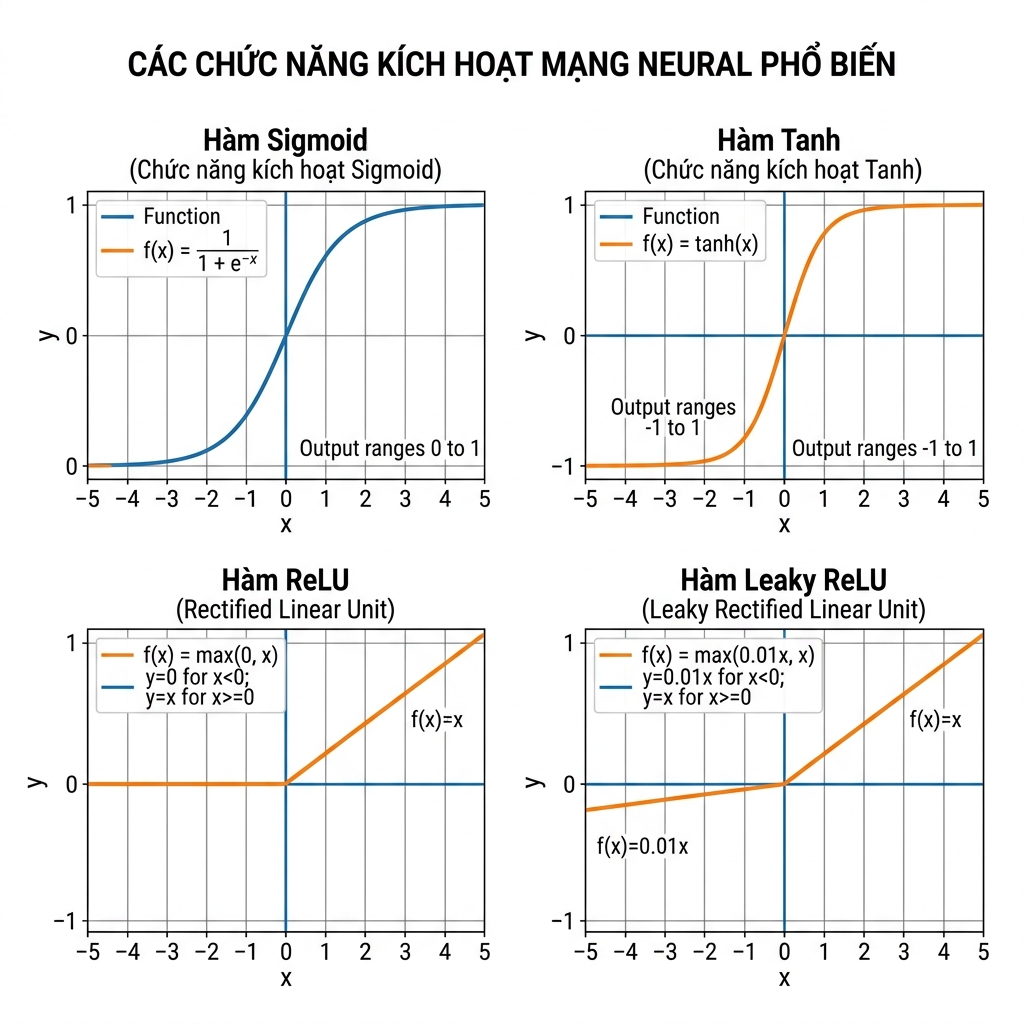
\includegraphics[width=0.75\textwidth]{figChap1/activation_functions.png}
    \caption{So sánh các hàm kích hoạt phổ biến trong CNN}
    \label{fig:activation_functions}
\end{figure}
    \noindent\textit{Chú thích:} Sigmoid, Tanh, ReLU và Leaky ReLU. ReLU và Leaky ReLU được ưa chuộng trong các kiến trúc hiện đại nhờ khả năng giảm thiểu vanishing gradient \cite{Nair2010, Maas2013}


\subsection{Các Kỹ thuật Chuẩn hóa}

Quá trình chuẩn hóa (Normalization) được sinh ra để cân bằng các giá trị tính toán trước hoặc sau kích hoạt nhằm hạn chế hội chứng nhảy loạn trong biểu diễn tri thức. Đây là một cơ chế thiết yếu để gia tốc sự hội tụ:
\begin{itemize}
    \item \textbf{Batch Normalization (BN):} Lấy trung bình và chuẩn hóa trên trục lô (mini-batch) \cite{Ioffe2015} nhằm giảm hiện tượng Internal Covariate Shift. Kỹ thuật này bị lệ thuộc nhiều vào kích thước batch nên khi tính toán bằng phần cứng hạn chế mức RAM sẽ nảy sinh lỗi thống kê.
    \item \textbf{Layer Normalization (LN):} Khác biệt với BN \cite{Ba2016} ở chỗ lấy phương sai toàn cục của kênh trong một mẫu ảnh nhất định, không chịu tác động nhỏ lẻ trên batch. Kỹ thuật này thường được áp dụng cho Transformers hay RNNs.
    \item \textbf{Group Normalization (GN):} Một sự dung hòa \cite{Wu2018}, chia bộ các bản đồ đặc trưng làm nhiều nhóm nhỏ có số kênh chuyên biệt để lấy kết quả trên mạng tích chập mà không làm phụ thuộc chiều lô mạng lưới hệ thống.
    \item \textbf{Instance Normalization (IN):} Xử lý chuẩn hóa theo mức độ cụ thể nhất \cite{Ulyanov2016} – với mỗi mẫu ảnh và mỗi kênh độc lập. Kỹ thuật này ngăn chặn các thông tin toàn cục làm lu mờ phong cách nội tải và là sự lựa chọn hoàn hảo bên trong ứng dụng chuyển đổi hình ảnh. Đặc biệt \textbf{quan trọng vì LADE (sẽ trình bày ở Chương 2) là quá trình cải tiến nâng cao trên nền Instance Normalization.}
\end{itemize}

\begin{figure}[H]
    \centering
    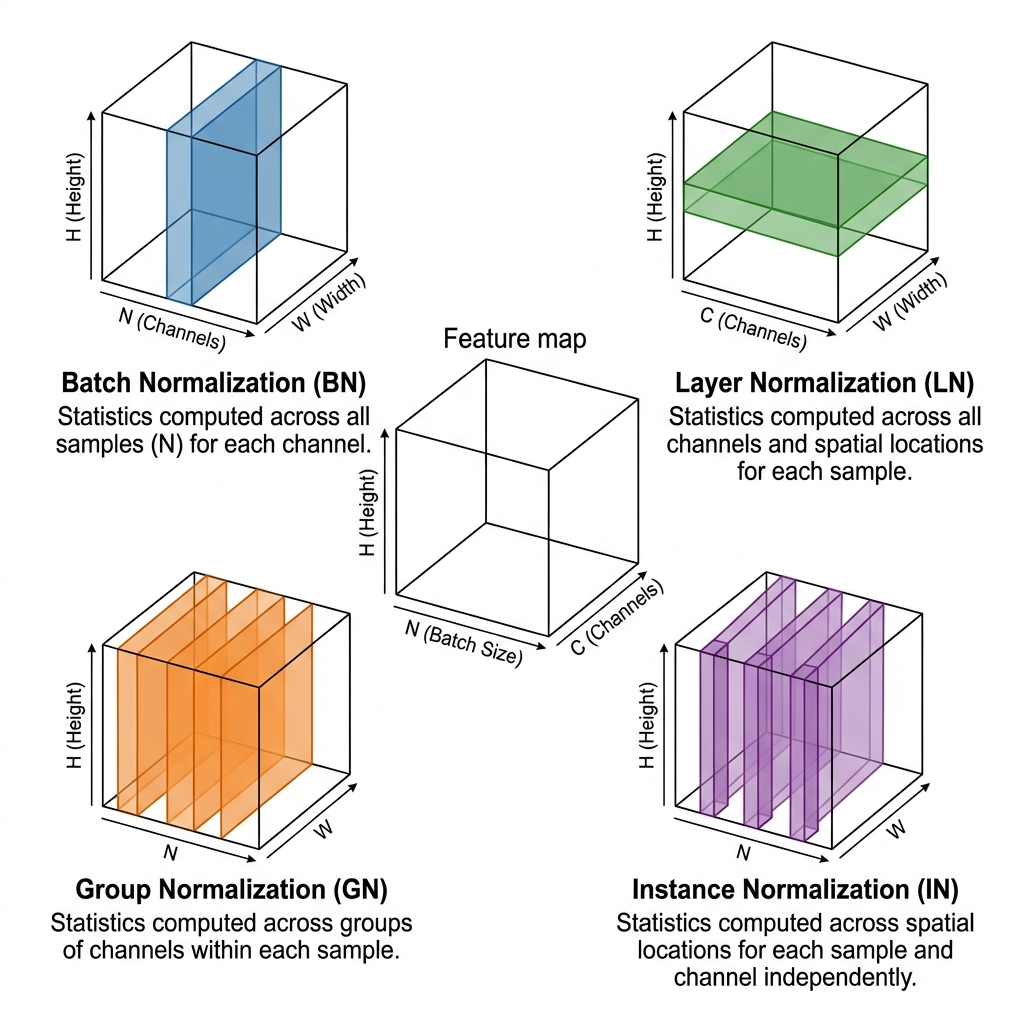
\includegraphics[width=0.85\textwidth]{figChap1/normalization_comparison.png}
    \caption{So sánh bốn kỹ thuật chuẩn hóa theo chiều không gian tính toán thống kê trên tensor đặc trưng $(N \times C \times H \times W)$}
    \label{fig:normalization_comparison}
\end{figure}
    \noindent\textit{Chú thích:} BN chuẩn hóa theo chiều batch $N$; LN theo toàn bộ kênh $C$ của một mẫu; GN theo nhóm kênh; IN theo từng kênh của từng mẫu độc lập \cite{Wu2018, Ulyanov2016}


\subsection{Spectral Normalization (SN)}

Spectral Normalization (SN) \cite{Miyato2018} là kỹ thuật áp dụng công thức chuẩn hóa ma trận khối lượng $W$, kìm hãm chỉ số biến thiên cao nhất bằng cách chia nó cho giá trị riêng lớn nhất (Largest singular value). \textbf{Được dùng trong Discriminator — tham chiếu \texttt{spectral\_norm()}}. Khi ứng dụng kết hợp trong các Mạng Phân biệt (Discriminator), SN đáp ứng các ràng buộc Lipschitz nhằm ổn định hệ thống.

\subsection{Sự Phát triển Kiến trúc và Nguyên lý Thiết kế Sâu}

\subsubsection{Các Cột mốc phát triển và Ý nghĩa của Độ sâu Mạng}

Sự trỗi dậy của CNN trong thị giác máy tính hiện đại được đánh dấu bằng các kiến trúc cột mốc.
AlexNet, được phát triển vào năm 2012, là mô hình CNN sâu đầu tiên được công nhận rộng rãi,
nổi bật qua thành tích trong Thử thách Nhận dạng Hình ảnh Quy mô Lớn ImageNet (ILSVRC).
AlexNet đã chứng minh một cách dứt khoát rằng độ sâu của mô hình là yếu tố thiết yếu để đạt 
hiệu suất cao, điều này chỉ trở nên khả thi nhờ vào việc tận dụng đơn vị xử lý đồ họa (GPUs) 
để giảm chi phí tính toán khi huấn luyện. \cite{WikiAlexNet}
\begin{figure}[H]
    \centering
    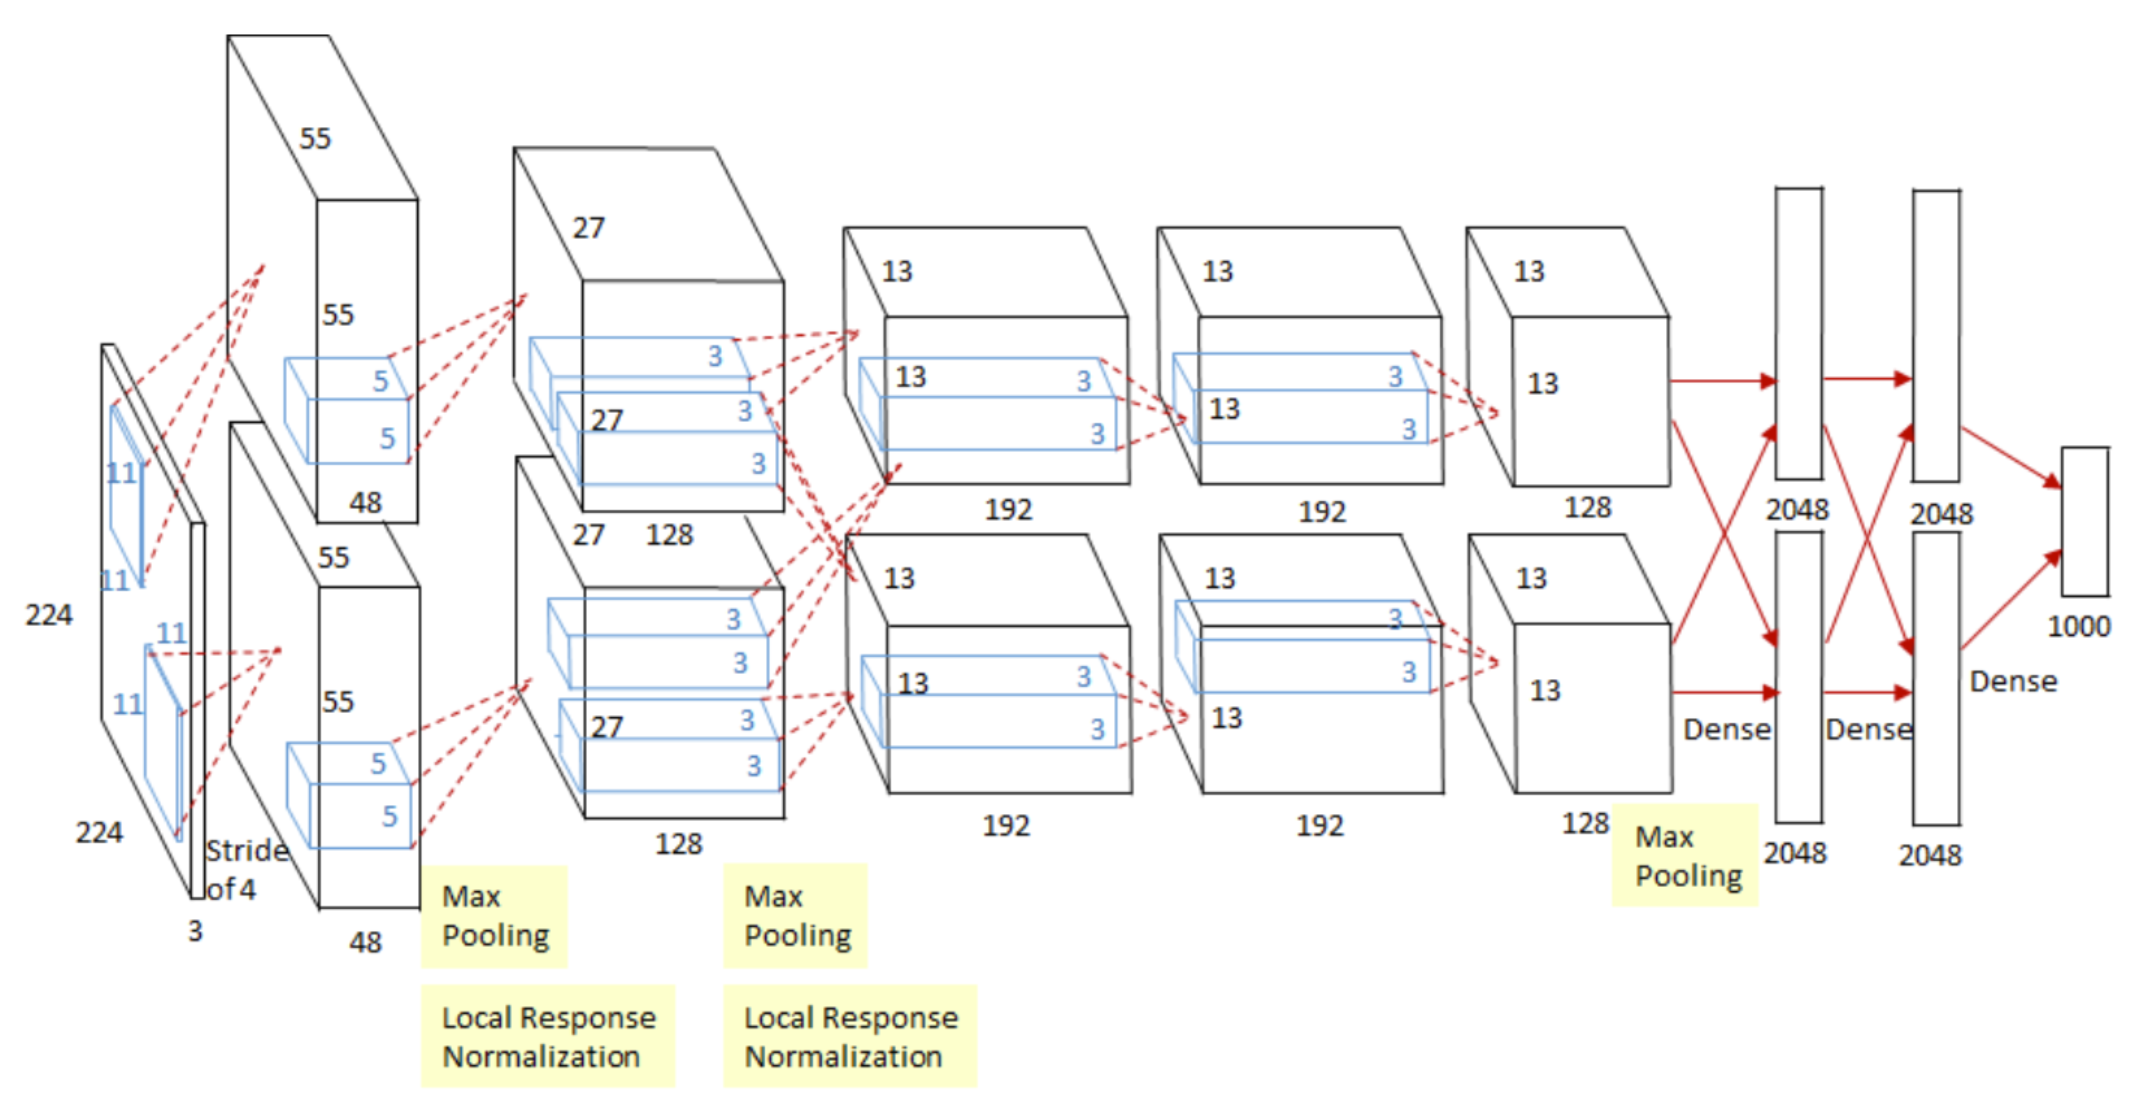
\includegraphics[width=0.8\textwidth]{figChap1/alexNet.png}
    \caption{Kiến trúc AlexNet}
    \label{fig:alexnet}
\end{figure}
    \noindent\textit{Chú thích:} Mô hình CNN sâu đầu tiên đạt kết quả dẫn đầu tại ILSVRC 2012, gồm 5 lớp tích chập và 3 lớp kết nối đầy đủ \cite{WikiAlexNet}


Sau thành công ban đầu, các kiến trúc tiếp theo (như VGGNet) tiếp tục đẩy giới hạn về độ sâu. Đồng thời, nghiên cứu cũng tập trung vào việc tối ưu hóa hiệu suất và tham số. Việc đơn giản hóa các kiến trúc dựa trên LeNet đã đạt được những giảm thiểu đáng kể về độ phức tạp tính toán và số lượng tham số trong khi vẫn duy trì hiệu suất cạnh tranh \cite{Basha2020}. Điều này nhấn mạnh tiềm năng của các kiến trúc hiệu quả (efficient architectures) trong việc giải quyết các ràng buộc phần cứng trong ứng dụng thực tế.

\subsubsection{Chiến lược Chống Tắt Dần Gradient: Inception và Residual Connections}

Khi các mạng trở nên sâu hơn, vấn đề tắt dần gradient (vanishing gradients) và khó khăn 
trong tối ưu hóa đã thúc đẩy sự ra đời của các chiến lược kiến trúc mới.

Kiến trúc Inception nổi bật vì khả năng đạt hiệu suất rất tốt với chi phí tính toán tương 
đối thấp. Sau đó, sự giới thiệu của kết nối residual (hay skip connections) trong ResNet đã 
mang lại hiệu suất dẫn đầu (state-of-the-art) vào năm 2015. Điều này đặt ra câu hỏi về 
lợi ích của việc kết hợp kiến trúc Inception với kết nối residual. \cite{Szegedy2017}

Nghiên cứu về Inception-ResNet đã cung cấp bằng chứng thực nghiệm rõ ràng rằng việc huấn 
luyện với kết nối residual tăng tốc đáng kể quá trình huấn luyện của mạng Inception.\cite{Szegedy2017}
Lợi ích này không chỉ là lý thuyết; kỹ thuật DropIn, một phương pháp dần dần cho phép 
đào tạo trực tiếp các mạng sâu và khó huấn luyện như VGG16, cho thấy sự cải thiện đáng 
kể trong độ chính xác của mạng.\cite{Radford2015}

\begin{figure}[H]
    \centering
    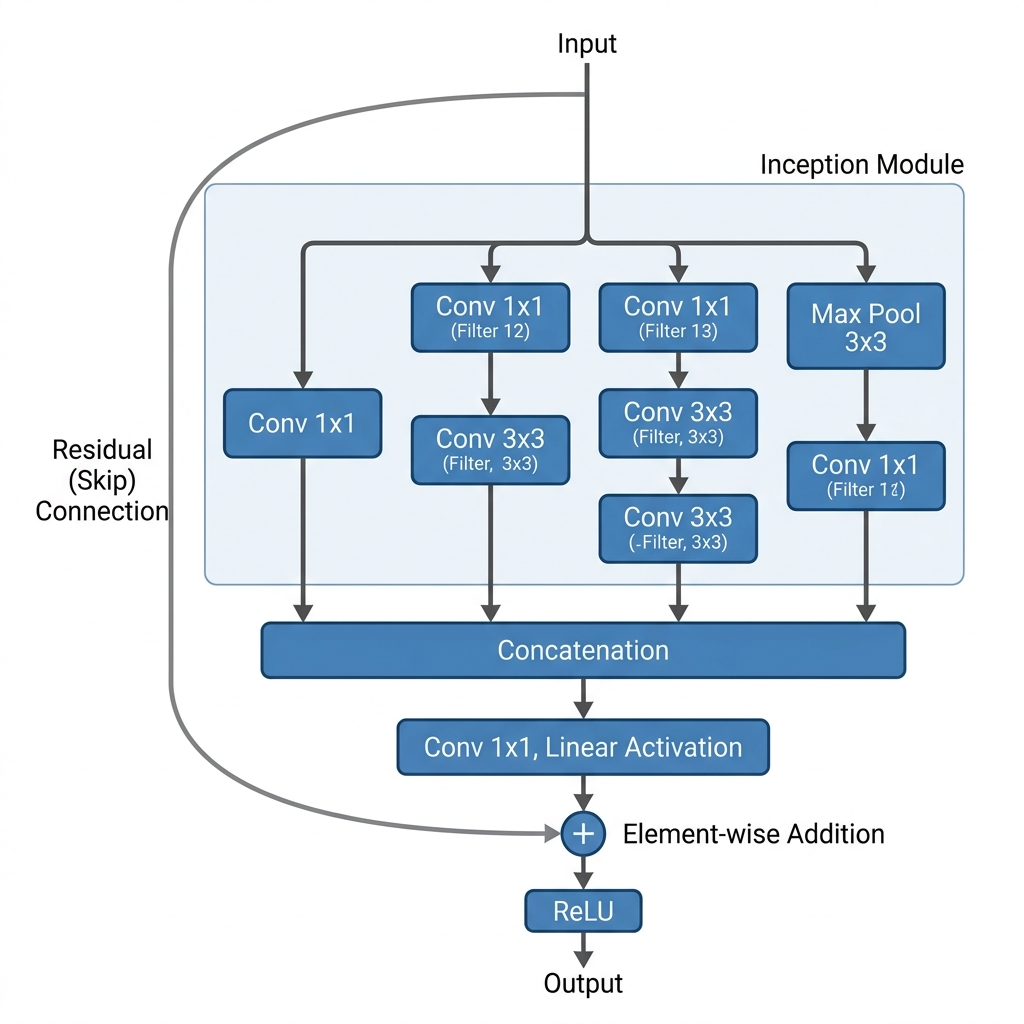
\includegraphics[width=0.65\textwidth]{figChap1/inception_resnet_block.png}
    \caption{Kiến trúc khối Inception-ResNet}
    \label{fig:inception_resnet_block}
\end{figure}
    \noindent\textit{Chú thích:} Kết hợp mô-đun Inception đa nhánh (Conv $1{\times1$, $3{\times}3$, $5{\times}5$ và Max Pooling) với kết nối residual (skip connection). Phép cộng theo phần tử (element-wise addition) sau tích chập $1{\times}1$ tuyến tính giúp ổn định huấn luyện mạng rất sâu \cite{Szegedy2017}.}


Các biến thể Inception-ResNet (như v1 và v2) đã được thiết kế lại để sử dụng các 
khối Inception rẻ hơn. Để bù đắp cho việc giảm chiều (dimensionality reduction) do khối 
Inception gây ra trước khi thực hiện phép cộng residual, một lớp mở rộng bộ lọc 
(filter-expansion layer), sử dụng tích chập $1 \times 1$ không có hàm kích hoạt, 
đã được thêm vào sau mỗi khối Inception. Ngoài ra, việc sử dụng kỹ thuật Activation Scaling 
cũng được chứng minh là cần thiết để ổn định quá trình huấn luyện các mạng Inception 
residual rất rộng. Mặc dù các nhà nghiên cứu đã chứng minh rằng việc huấn luyện các mạng 
rất sâu mà không cần kết nối residual là khả thi, lợi thế về tốc độ tối ưu hóa mà kết nối 
residual mang lại là một lý do kỹ thuật mạnh mẽ để chúng được áp dụng rộng rãi.\cite{Szegedy2017}

\subsubsection{Nguyên tắc Thiết kế Kiến trúc dựa trên Dữ liệu và Tối ưu hóa FC}

Việc lựa chọn kiến trúc CNN (sâu hay nông) không nên chỉ dựa trên kinh nghiệm mà phải 
tương quan với đặc điểm của tập dữ liệu đang được sử dụng. Các tập dữ liệu có thể được 
phân loại là sâu (deeper), nghĩa là chúng có số lượng mẫu lớn trên mỗi lớp (ví dụ: CIFAR-10), 
hoặc rộng (wider), nghĩa là chúng có nhiều lớp nhưng ít mẫu hơn trên mỗi 
lớp (ví dụ: CIFAR-100, Tiny ImageNet).\cite{Basha2020}
Nghiên cứu đã chỉ ra các quy tắc thiết kế mang tính hướng dẫn như sau:

\begin{enumerate}
    \item Dữ liệu Sâu (Deeper Datasets): Các tập dữ liệu này phù hợp hơn với các kiến trúc 
    CNN sâu (ví dụ: CNN-2 và CNN-3). Do các kiến trúc sâu có nhiều tham số có thể huấn luyện 
    hơn, chúng cần số lượng hình ảnh lớn trên mỗi chủ thể để huấn luyện hiệu quả. Các kiến 
    trúc sâu hơn đã chứng minh hiệu suất tốt hơn trên các tập dữ liệu sâu như CIFAR-10 và 
    CRCHistoPhenotypes.\cite{Basha2020}
    \item Dữ liệu Rộng (Wider Datasets): Các tập dữ liệu này hoạt động hiệu quả hơn với các 
    kiến trúc CNN nông (ví dụ: CNN-1). Mạng nông có ít tham số hơn, điều này phù hợp hơn với 
    các tập dữ liệu có sự đa dạng lớp lớn nhưng số lượng mẫu trên mỗi lớp bị hạn chế.\cite{Basha2020}
\end{enumerate}

Mối quan hệ giữa độ sâu kiến trúc và thiết kế lớp FC cũng tuân theo logic này. 
Mạng nông cần nhiều nơ-ron và lớp FC hơn để tổng hợp các đặc trưng, trong khi mạng sâu 
cần ít nơ-ron FC hơn. Việc xác định mối quan hệ qua lại này cung cấp một khuôn khổ khoa 
học giúp các nhà phát triển lựa chọn kiến trúc tối ưu hóa hiệu suất và chi phí tính toán 
ngay từ đầu, giảm thiểu quá trình thử và sai tốn thời gian.

\begin{table}[H]
    \centering
    \caption{Lựa chọn Kiến trúc và Tối ưu hóa Lớp FC} % Có thể đổi tên caption tùy ý
    \label{tab:ds_bophan}
    
    % Cấu trúc cột: |c|c|c|c|c|p{...}|
    % c: Căn giữa | p{3.5cm}: Cột kiểu paragraph với chiều rộng 3.5cm
    \begin{tabular}{|c|c|c|p{3.5cm}|} 
        \hline
        \textbf{Kiến trúc CNN} & \textbf{Đặc điểm Tập dữ liệu Tối ưu} & \textbf{Yêu cầu Lớp FC} & \textbf{Lý do Kỹ thuật} \\
        \hline
        
        Sâu (Deeper) & Sâu (Nhiều mẫu/lớp) & Thấp (Ít nơ-ron/lớp) &  Đặc trưng trừu tượng hóa cao, giảm gánh nặng tính toán trong giai đoạn quyết định. \\
        \hline
        
        Nông (Shallow) & Rộng (Nhiều lớp, ít mẫu/lớp) & Cao (Nhiều nơ-ron/lớp) &  Bù đắp cho đặc trưng ít trừu tượng, mô hình có ít tham số hơn, phù hợp với sự đa dạng lớp. \\
        \hline
        
    \end{tabular}
\end{table}

\subsection{Kiến trúc CNN cho Tác vụ Định vị và Phân đoạn Mật độ cao}

\subsubsection{Phân đoạn Thực thể (Instance Segmentation) với Mask R-CNN}

Trong khi các kiến trúc như AlexNet và ResNet tập trung vào phân loại, các tác vụ thị giác 
máy tính phức tạp hơn như phân đoạn thực thể đòi hỏi độ chính xác không gian cao. 
Mask R-CNN là một khung làm việc linh hoạt và đơn giản về mặt khái niệm, mở rộng Faster 
R-CNN để không chỉ phát hiện đối tượng mà còn đồng thời tạo ra mặt nạ phân đoạn chất lượng 
cao cho mỗi thực thể. \cite{He2017}

Mask R-CNN duy trì quy trình hai giai đoạn của Faster R-CNN, nhưng ở giai đoạn thứ hai, 
nó bổ sung một nhánh thứ ba hoạt động song song với nhánh dự đoán hộp giới hạn 
(bounding-box) và phân loại. Nhánh này là một Mạng Tích chập Đầy đủ (Fully Convolutional 
Network – FCN) nhỏ, được áp dụng trên từng Vùng Quan tâm (Region of Interest – RoI) để dự 
đoán một mặt nạ phân đoạn $m \times m$ theo cách pixel-to-pixel. \cite{He2017}
\begin{figure}[H]
    \centering
    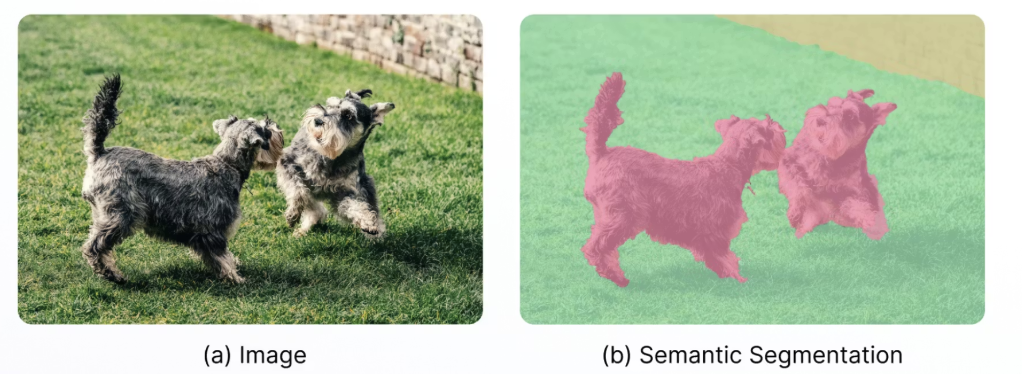
\includegraphics[width=0.8\textwidth]{figChap1/phan_doan_thuc_the.png}
    \caption{Phân đoạn Thực thể}
    \label{fig:phan_doan_thuc_the}
\end{figure}

\textbf{Lớp RoIAlign và Căn chỉnh Chính xác}: 
Thành phần kỹ thuật quan trọng nhất làm nên sự thành công của Mask R-CNN là việc giới thiệu lớp 
RoIAlign. Faster R-CNN sử dụng lớp RoIPooling, lớp này thực hiện lượng tử hóa (spatial 
quantization) thô, dẫn đến sự sai lệch (misalignment) giữa input của mạng và output 
pixel-to-pixel, gây ảnh hưởng tiêu cực đến độ chính xác không gian.\cite{He2017}

RoIAlign khắc phục vấn đề này bằng cách là một lớp không lượng tử hóa \\(quantization-free), 
duy trì căn chỉnh vị trí chính xác. Nó tính toán giá trị của các điểm lấy mẫu bằng cách sử 
dụng nội suy song tuyến (bilinear interpolation) từ các điểm lưới gần kề trên bản đồ đặc trưng, 
loại bỏ hoàn toàn việc lượng tử hóa các tọa độ liên quan. Sự thay đổi dường như nhỏ này đã mang 
lại tác động lớn, cải thiện độ chính xác mặt nạ lên đến $10\%$ đến $50\%$, đặc biệt quan trọng 
dưới các tiêu chí định vị nghiêm ngặt.\cite{He2017}

\textbf{Decoupling Mask Prediction}: Một yếu tố kỹ thuật khác là việc tách rời (decoupling) 
dự đoán mặt nạ và dự đoán lớp. Thay vì sử dụng softmax và loss đa thức (multinomial loss) 
khiến các mặt nạ cạnh tranh lẫn nhau (phổ biến trong semantic segmentation), Mask R-CNN sử 
dụng sigmoid per-pixel và định nghĩa loss mặt nạ ($L_{mask}$) chỉ trên mặt nạ lớp đúng của 
RoI đó. Cách tiếp cận này đã được chứng minh là chìa khóa để đạt được kết quả phân đoạn 
thực thể tốt.\cite{He2017}

Sự thành công của Mask R-CNN chứng minh rằng các tác vụ định vị mật độ cao đòi hỏi mức độ 
chính xác không gian cao hơn nhiều so với các tác vụ phát hiện hộp giới hạn đơn thuần. 
Khung làm việc này cũng linh hoạt, dễ dàng tổng quát hóa sang các tác vụ khác như ước tính 
tư thế người (person keypoint detection) bằng cách xem mỗi điểm khóa (keypoint) là một mặt nạ 
nhị phân one-hot.

\subsubsection{Mô hình Encoder-Decoder cho Tái tạo Hình ảnh Chất lượng cao (U-Net)}
Các kiến trúc Encoder-Decoder, nổi bật là U-Net, là nền tảng cho nhiều bài toán dịch ảnh 
(image-to-image translation) và phân đoạn mật độ cao. Phần encoder (sử dụng các lớp tích 
chập và pooling) nén ảnh gốc thành một vector đặc trưng ẩn, trong khi phần decoder tái 
tạo vector ẩn đó thành ảnh đầu ra mong muốn.\cite{Hasan2019}

\begin{figure}[H]
    \centering
    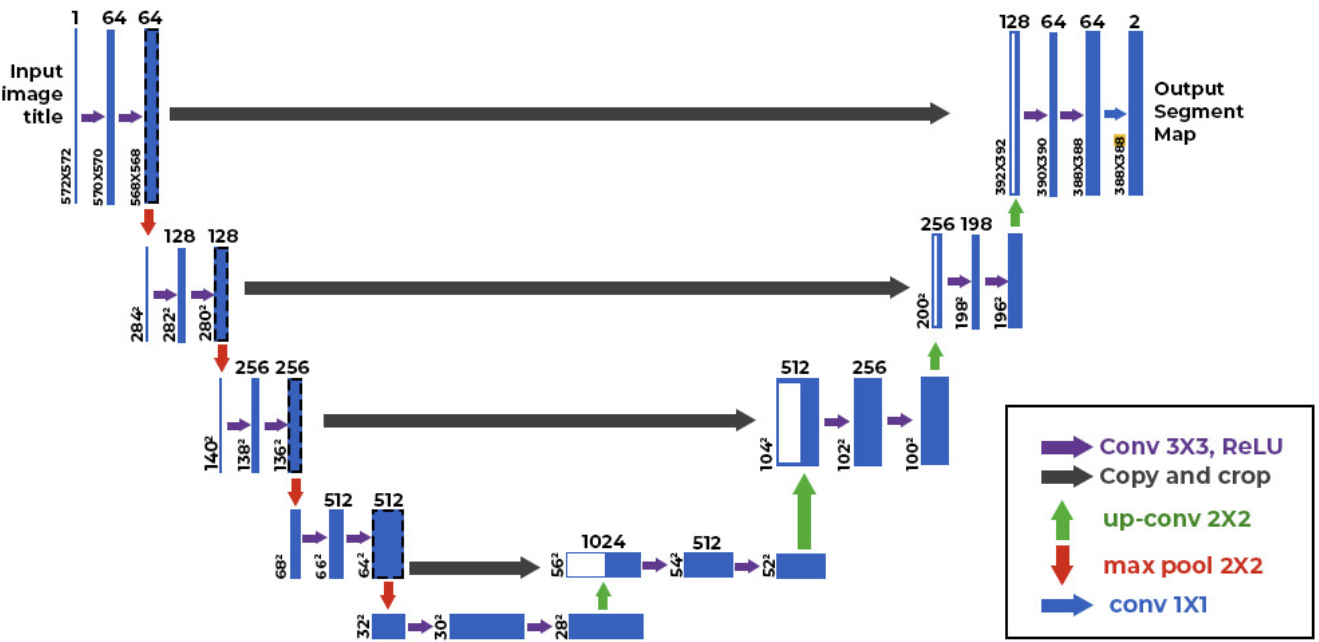
\includegraphics[width=0.9\textwidth]{figChap1/u-net.png}
    \caption{Mô hình U-Net}
    \label{fig:u-net}
\end{figure}

Trong phần decoder, việc tái tạo độ phân giải không gian thường được thực hiện bằng cách sử 
dụng Transposed Convolution (còn gọi là deconvolution hoặc tích chập chuyển vị). Mặc dù 
Transposed Convolution là một lớp học được, nó có một hạn chế kỹ thuật lớn: dễ dẫn đến sự 
chồng lấp không đều (uneven overlap), tạo ra các tạo phẩm (artifacts) dưới dạng mẫu kẻ ô 
(checkerboard-like patterns) trên đầu ra.\cite{Hasan2019}

Để giải quyết vấn đề này, mô hình U-NetPlus, được thiết kế cho phân đoạn công cụ phẫu thuật, 
đã giới thiệu một sự thay thế quan trọng. U-NetPlus sử dụng các encoder tiền huấn luyện 
(pre-trained), cụ thể là VGG-11 hoặc VGG-16, để tăng tốc độ hội tụ và cải thiện kết quả. 

Quan trọng hơn, trong phần decoder, U-NetPlus đã thay thế hoàn toàn Transposed Convolution 
bằng Nearest-Neighbor (NN) interpolation. Thao tác NN upsampling, theo sau là hai lớp tích chập, 
đã loại bỏ hiệu quả các tạo phẩm do Transposed Convolution gây ra, đồng thời giảm số lượng 
tham số của mô hình. Việc các nhà nghiên cứu lựa chọn một phương pháp nội suy không học được 
(NN) thay vì một lớp học được (Transposed Conv) để ổn định đầu ra decoder cho thấy rằng trong 
các miền ứng dụng nhạy cảm như y học, độ trung thực hình ảnh và tính ổn định đầu ra có thể được 
ưu tiên hơn khả năng học tối đa của mạng.\cite{Hasan2019}

\begin{table}[H]
\caption{Các Kỹ thuật Upsampling trong Decoder của CNN}
\label{tab:upsampling_techniques}
\centering
\begin{tabular}{|p{3.5cm}|p{3cm}|p{4.5cm}|p{4.5cm}|}
\hline
\textbf{Kỹ thuật} & \textbf{Đặc điểm} & \textbf{Ưu điểm Kỹ thuật} & \textbf{Hạn chế Kỹ thuật Chính} \\
\hline
Transposed Convolution & Học được (Learnable) & Linh hoạt, có thể học được bộ lọc tái tạo tối ưu. & Dễ gây ra tạo phẩm kiểu checkerboard do uneven overlap. \\
\hline
Nearest-Neighbor Interpolation & Không học được (Non-Learnable) & Giảm thiểu tạo phẩm, giảm số lượng tham số, ổn định đầu ra. & Độ mịn không gian có thể thấp, không học được sự tinh chỉnh chi tiết. \\
\hline
\end{tabular}
\end{table}


\subsection{CNNs trong Dịch Ảnh và Thích ứng Miền}
CNN không chỉ được sử dụng cho phân loại và phân đoạn, mà còn là nền tảng của các mô hình 
encoder-decoder dùng trong các bài toán dịch ảnh giữa các miền khác nhau (image-to-image 
translation).

\subsubsection{Dịch Ảnh Không Giám sát và Giả định Không gian Ẩn Chung}
Bài toán dịch ảnh không giám sát (Unsupervised Image-to-image translation) là một thách thức 
lớn vì chỉ có các bộ dữ liệu biên độc lập ($X_1, X_2$).\cite{Liu2017} Sự thiếu vắng các cặp 
ảnh tương ứng khiến việc suy luận về phân phối chung giữa hai miền trở nên không giải được 
(ill-posed problem) nếu không có các giả định bổ sung.

Để giải quyết vấn đề này, khung làm việc UNIT (UNsupervised Image-to-image Translation) đã được 
đề xuất, kết hợp Variational Autoencoders (VAEs) và Generative Adversarial Networks (GANs), 
dựa trên Giả định Không gian Ẩn Chung (Shared-Latent Space Assumption).

Giả định này khẳng định rằng một cặp ảnh tương ứng từ hai miền khác nhau 
($\text{x}_1, \text{x}_2$) có thể được ánh xạ tới cùng một biểu diễn ẩn ($\text{z}$) trong 
một không gian ẩn chung ($\text{Z}$). Về mặt toán học, điều này ngụ ý rằng tồn tại các hàm 
mã hóa $\text{E}^*_1, \text{E}^*_2$ và hàm sinh $\text{G}^*_1, \text{G}^*_2$ sao 
cho $\text{z} = \text{E}^*_1(\text{x}_1) = \text{E}^*_2(\text{x}_2)$ và $\text{x}_1 = \text{G}^*_1(\text{z})$, $\text{x}_2 = \text{G}^*_2(\text{z})$.\cite{Liu2017}

% \begin{figure}[H]
%     \centering
%     \begin{minipage}{0.28\textwidth} 
%         \centering
%         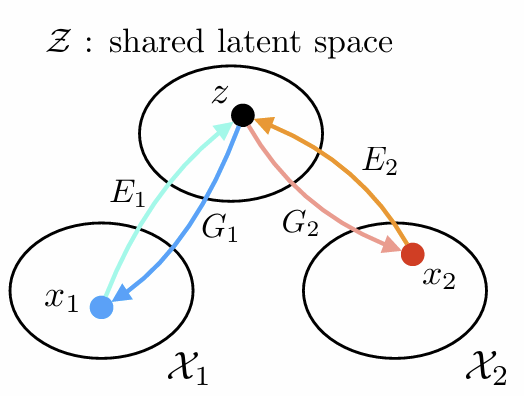
\includegraphics[width=\linewidth]{figChap1/image2imageUnsupervice-a.png} 
%         \caption{(a) Giả định không gian tiềm ẩn chia sẻ.}
%         \label{fig:shared_latent}
%     \end{minipage}
%     \hfill 
%     \begin{minipage}{0.68\textwidth} 
%         \centering
%         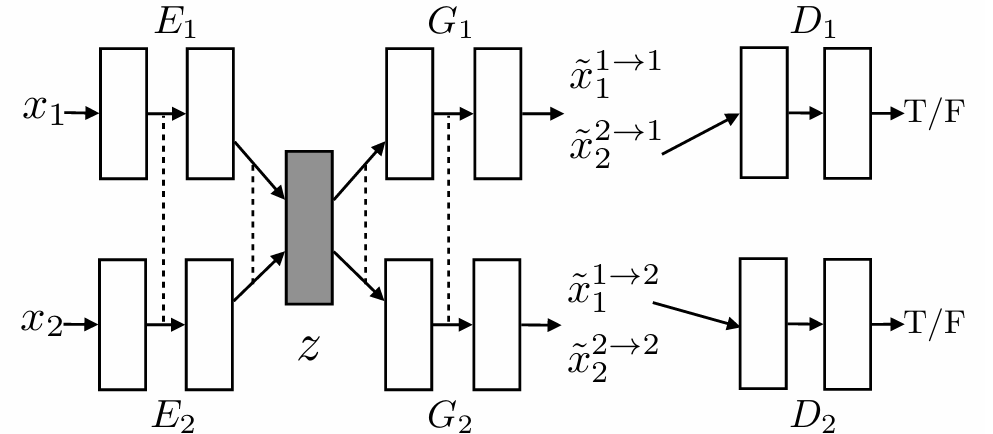
\includegraphics[width=\linewidth]{figChap1/image2imageUnsupervice-b.png}
%         \caption{(b) Khung công việc UNIT được đề xuất.}
%         \label{fig:unit_framework}
%     \end{minipage}
    
%     \caption{Không gian tiềm ẩn chia sẻ và kiến trúc mạng UNIT.}
%     \label{fig:unit_combined}
% \end{figure}

\begin{figure}[H]
    \centering
    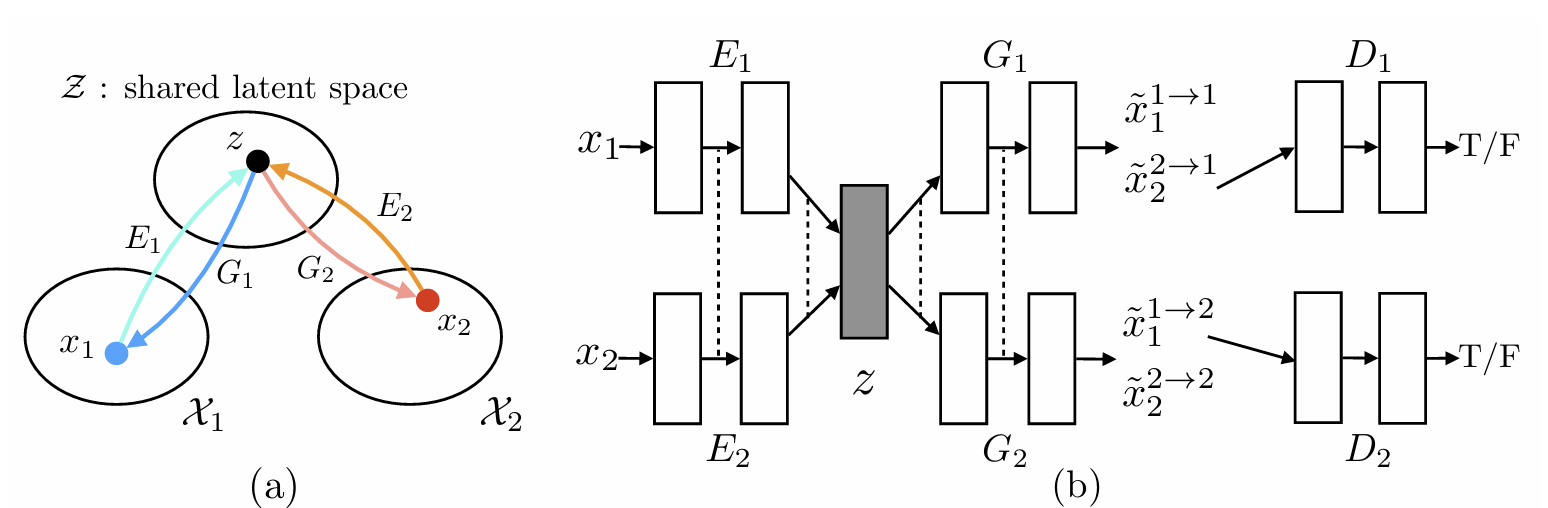
\includegraphics[width=\textwidth]{figChap1/image2imageUnsupervice.png} 
    
    \caption{Không gian tiềm ẩn chia sẻ và kiến trúc mạng UNIT.}
    \label{fig:unit_framework}
\end{figure}

\textbf{(a) Giả định không gian tiềm ẩn chia sẻ.} Chúng ta giả định một cặp hình 
ảnh tương ứng $(x_1, x_2)$ trong hai miền khác nhau $\mathcal{X}_1$ và $\mathcal{X}_2$ có 
thể được ánh xạ tới cùng một mã tiềm ẩn $z$ trong không gian tiềm ẩn chia sẻ 
$\mathcal{Z}$. $E_1$ và $E_2$ là hai hàm mã hóa, ánh xạ hình ảnh tới các mã tiềm ẩn. 
$G_1$ và $G_2$ là hai hàm tạo sinh, ánh xạ các mã tiềm ẩn trở lại hình ảnh. 
\textbf{(b) Khung công việc UNIT được đề xuất.} Chúng ta biểu diễn 
$E_1, E_2, G_1$ và $G_2$ bằng cách sử dụng Mạng nơ-ron tích chập (CNN) và thực hiện
giả định không gian tiềm ẩn chia sẻ bằng cách sử dụng ràng buộc chia sẻ trọng số,
nơi trọng số kết nối của vài lớp đầu tiên (các lớp cấp cao) trong $E_1$ và $E_2$ được 
gắn kết với nhau (minh họa bằng các đường đứt nét) và trọng số kết nối của vài lớp đầu 
tiên trong $G_1$ và $G_2$ cũng được gắn kết với nhau. Ở đây, $\tilde{x}_1^{1 \to 1}$ 
và $\tilde{x}_2^{2 \to 2}$ là các hình ảnh tự tái tạo, và $\tilde{x}_1^{1 \to 2}$ 
và $\tilde{x}_2^{2 \to 1}$ là các hình ảnh đã được chuyển miền. $D_1$ và $D_2$ là các 
bộ phân biệt đối kháng (adversarial discriminator) cho các miền tương ứng, có nhiệm vụ 
đánh giá xem các hình ảnh đã được chuyển có thực tế hay không.

\subsubsection{Cơ chế Triển khai Không gian Ẩn Chung trong UNIT}

Trong UNIT, giả định Shared-Latent Space được triển khai thông qua ràng buộc chia sẻ trọng số 
(weight-sharing constraint) giữa các mạng con. 
\begin{itemize}
\item Encoders ($\text{E}_1, \text{E}_2$): Các trọng số của vài lớp cuối cùng (các lớp cấp cao) 
trong hai Encoders được ràng buộc chia sẻ. Những lớp này có trách nhiệm trích xuất các đặc trưng 
biểu diễn cấp cao.\cite{Liu2017}
\item Generators ($\text{G}_1, \text{G}_2$): Tương tự, các trọng số của vài lớp đầu tiên 
(các lớp cấp cao) trong hai Generators được ràng buộc chia sẻ.\cite{Liu2017}
\end{itemize}
Ràng buộc chia sẻ trọng số này là cơ chế vật lý hóa giả định không gian ẩn chung, buộc các 
Encoders phải ánh xạ các ảnh tương ứng vào cùng một mã ẩn. 

Giả định không gian ẩn chung cũng ngầm định yêu cầu tính nhất quán vòng lặp 
(cycle-consistency constraint), đảm bảo rằng một hình ảnh được dịch từ miền $X_1$ 
sang $X_2$ và sau đó được dịch trở lại $X_1$ sẽ gần giống với hình ảnh gốc 
($\text{x}_1 = \text{G}^*_1(\text{E}^*_2(\text{G}^*_2(\text{E}^*_1(\text{x}_1))))$).\cite{Liu2017} 
Sự kết hợp giữa VAEs (để tái tạo ảnh), GANs (để đảm bảo ảnh dịch là thực tế) 
và ràng buộc chia sẻ trọng số (để liên kết các miền) cho phép CNN hoạt động như 
một nền tảng trích xuất và tái tạo nội dung, thành công trong nhiều tác vụ dịch ảnh phức tạp.

\subsubsection{Thích ứng Miền (Domain Adaptation) thông qua Style Transfer}

Khả năng học đặc trưng trừu tượng của CNN cũng được sử dụng để giải quyết vấn đề thích ứng 
miền (domain adaptation), đặc biệt khi có sự dịch chuyển miền (domain shift) — tức là khi 
dữ liệu huấn luyện (nguồn) và dữ liệu thử nghiệm (đích) đến từ các phân phối khác nhau 
(ví dụ: ảnh chụp ban ngày so với ban đêm, hoặc ảnh không sương mù so với có sương mù).\cite{WangLAST}

Sự dịch chuyển miền gây ra sự suy giảm hiệu suất đáng kể. Ví dụ, trong bài toán phân đoạn ảnh 
trên không (aerial image segmentation), sự dịch chuyển miền gây ra mức giảm trung 
bình $-5.22\%$ mIoU trên bộ dữ liệu Potsdam.\cite{WangLAST} Để chống lại sự suy giảm này, 
một mô hình chuyển phong cách trong không gian ẩn (latent space style transfer model) đã 
được đề xuất.\cite{WangLAST} Mô hình này sử dụng các biểu diễn đặc trưng ẩn của CNN để tạo 
ra các phiên bản dữ liệu tổng hợp với phong cách miền đích (ví dụ: thêm sương mù vào ảnh rõ nét).

Cách tiếp cận này loại bỏ nhu cầu ghi chú bổ sung (annotation) trên dữ liệu miền dịch 
chuyển.\cite{WangLAST} Bằng cách áp dụng phương pháp này, hiệu suất trên miền 
dịch chuyển đã được cải thiện đáng kể (ví dụ: tăng $+3.97\%$ mIoU trên Potsdam), 
chứng minh rằng việc sử dụng CNN để trích xuất và thao túng các đặc trưng phong cách 
trừu tượng là một chiến lược hiệu quả để nâng cao tính tổng quát của mô hình trong môi 
trường thực tế.

\subsection{Đánh giá và Xu hướng Tương lai của Kiến trúc Tích chập}

\subsubsection{Vị thế của CNN và Sự Cộng sinh với Vision Transformer}

Trong bối cảnh Vision Transformer (ViT) đang nổi lên như một đối thủ cạnh tranh mạnh mẽ, 
CNNs (như ResNet và ConvNeXt) vẫn duy trì vị thế là các mô hình nền tảng trong nghiên cứu 
thị giác máy tính. \cite{Lin2025}

Phân tích cho thấy CNNs vẫn thể hiện ưu thế hoặc hiệu suất tương đương với ViT, đặc biệt trong 
chế độ học ít mẫu (low-data few-shot regime) trong quá trình học chuyển giao (transfer learning). 
Điều này được cho là do CNNs sở hữu một thiên kiến quy nạp cục bộ (local inductive bias) vốn có, 
giúp chúng học ổn định hơn và cần ít dữ liệu hơn để khái quát hóa các mối quan hệ không gian cơ 
bản.

Xu hướng nghiên cứu hiện đại đang hướng tới các mô hình hỗn hợp (Hybrid), kết hợp các thành 
phần của CNN và Transformer để tận dụng ưu điểm của cả hai. Ví dụ, kiến trúc CoAtNet kết hợp 
các khối tích chập của CNN với cơ chế tự chú ý (self-attention) của Transformer, đạt hiệu suất
 tối ưu bằng cách cân bằng giữa việc xử lý thông tin cục bộ và bắt ngữ cảnh toàn cục.

\subsubsection{Ứng dụng trong Chẩn đoán Y tế và Ensemble Learning}

Lĩnh vực chẩn đoán y tế, như phân tích X-quang ngực, là một ứng dụng quan trọng đòi hỏi độ 
tin cậy và độ chính xác cao. Việc sử dụng các kỹ thuật học sâu (bao gồm các CNNs tiền huấn 
luyện, Transformer và mô hình Hybrid) đã được chứng minh là có ý nghĩa quan trọng trong việc 
tự động chẩn đoán các bệnh lý lồng ngực.

Trong các lĩnh vực có tính quyết định cao như y học, việc giảm thiểu rủi ro và tăng độ tin 
cậy là tối quan trọng. Nghiên cứu đã chứng minh rằng kỹ thuật tập hợp học sâu (Ensemble Deep 
Learning) có thể cải thiện đáng kể hiệu suất chẩn đoán.\cite{Lin2025} Bằng cách kết hợp 
dự đoán của nhiều mô hình đã huấn luyện (bao gồm cả CNNs truyền thống và mô hình hybrid như 
CoAtNet) thông qua trung bình có trọng số, hiệu suất đã được cải thiện, đạt AUROC $85.4\%$ 
trên bộ dữ liệu ChestX-ray14, vượt qua các phương pháp dẫn đầu khác.\cite{Lin2025} Điều 
này khẳng định rằng việc tổng hợp kết quả từ nhiều kiến trúc là một chiến lược quan trọng để 
tăng độ chính xác và độ tin cậy trong các ứng dụng thực tiễn.


\section{Kiến trúc Mạng đối nghịch tạo sinh}
Trong thập kỷ qua, Trí tuệ Nhân tạo (AI) đã chuyển dịch mạnh mẽ từ khả năng phân tích sang 
sáng tạo, với dấu mốc quan trọng là sự ra đời của Mạng Đối nghịch Tạo sinh (GAN) do Ian 
Goodfellow và cộng sự đề xuất năm 2014. Khác với các mô hình tạo sinh trước đây vốn dựa 
trên các phương pháp xác suất phức tạp như MCMC hay Deep Belief Networks, GAN đưa ra cách 
tiếp cận mới bằng trò chơi đối kháng giữa hai mạng nơ-ron, tận dụng lan truyền ngược để huấn 
luyện trực tiếp và tạo ra dữ liệu có độ trung thực cao.\cite{Goodfellow2014}

\subsection{Nguyên lý Hoạt động và Cơ sở Lý thuyết}
\subsubsection{Khung Làm việc Đối kháng}

GAN (Generative Adversarial Networks) là một hệ thống gồm hai mạng nơ-ron được huấn luyện đồng 
thời thông qua một trò chơi có tổng bằng không. Trong đó mạng Tạo sinh (Generator - G) đóng vai
trò như một ``kẻ làm giả''. G nhận đầu vào là một vector nhiễu ngẫu nhiên $z$ từ một không gian 
tiềm ẩn (latent space) với phân phối $p_z(z)$, để tạo ra phân phối chuẩn hoặc giống như phân 
phối dữ liệu thật $p_{data}$. G cố gắng tạo ra những mẫu gần khớp với $G(z)$. Mục tiêu của G 
là đánh lừa D, nghĩa là tạo ra những mẫu mà D không thể phân biệt được với dữ liệu 
thật $p_{data}$. Ngược lại mạng Phân biệt (Discriminator - D) đóng vai trò như một ``cảnh sát'' 
hoặc chuyên gia giám định. D là một bộ phân loại nhị phân nhận đầu vào là dữ liệu $x$ và xuất 
ra một giá trị thể hiện hướng $D(x; \theta_D)$ biểu thị xác suất dữ liệu đó là dữ liệu 
thật ($p_{data}$) thay vì từ G.\cite{Goodfellow2014}

\begin{figure}[H]
    \centering
    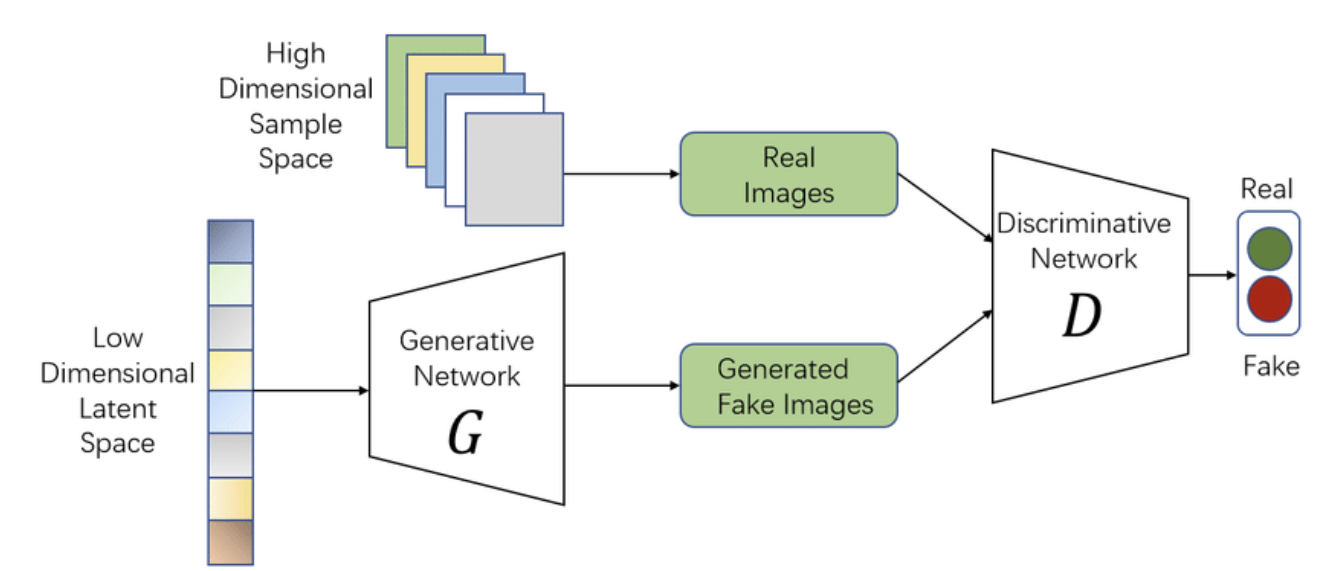
\includegraphics[width=0.85\textwidth]{figChap1/gan-architect.png}
    \caption{Kiến trúc tổng quát của Mạng Đối nghịch Tạo sinh (GAN)}
    \label{fig:gan}
\end{figure}
    \noindent\textit{Chú thích:} Mạng Generator $G$ nhận vector nhiễu $z \sim p_z(z)$ để tạo ra mẫu giả $G(z)$, trong khi Discriminator $D$ học phân biệt dữ liệu thật $x \sim p_{\text{data}$ với dữ liệu giả. Hai mạng được huấn luyện đồng thời theo trò chơi minimax \cite{Goodfellow2014}.}


\subsubsection{Trò chơi Minimax và Hàm Mục tiêu}
Quá trình huấn luyện GAN được mô hình hóa dưới dạng một bài toán tối ưu hóa Minimax, 
trong đó $D$ cố gắng tối đa hóa khả năng phân biệt đúng, còn $G$ cố gắng tối thiểu hóa khả 
năng bị phát hiện (tức là tối đa hóa sai sót của $D$). Hàm giá trị $V(D, G)$ được định nghĩa 
như sau:

\begin{equation}
\min_G \max_D V(D, G) = \mathbb{E}_{x \sim p_{\text{data}}(x)}[\log D(x)] + \mathbb{E}_{z \sim p_z(z)}[\log(1 - D(G(z)))]
\end{equation}
Trong đó số hạng đầu tiên $\mathbb{E}_{x \sim p_{\text{data}}(x)}$ khuyến khích $D$ gán xác suất 
cao cho dữ liệu thật.
Số hạng thứ hai $\mathbb{E}_{z \sim p_z(z)}$ khuyến khích $D$ gán xác suất thấp cho dữ liệu 
giả $G(z)$.\cite{Goodfellow2014}

\subsubsection{Phân tích Điểm Cân bằng Nash và Discriminator Tối ưu}
Về mặt lý thuyết, mục tiêu cuối cùng của quá trình này là đạt được Điểm cân bằng Nash 
(Nash Equilibrium). Tại điểm này, không người chơi nào có thể cải thiện kết quả của mình 
bằng cách đơn phương thay đổi chiến lược.\cite{Jabbar2021}
Đối với GAN, Discriminator không thể phân biệt được ảnh thật và ảnh giả tốt hơn việc đoán 
ngẫu nhiên (xác suất $D(x) = 0.5$ cho mọi $x$).
Phân phối của Generator $p_g$ hoàn toàn trùng khớp với phân phối dữ liệu thật $p_{data}$.

Goodfellow et al \cite{Goodfellow2014} đã chứng minh rằng với một $G$ cố định, Discriminator tối ưu $D^*$ có dạng:
\begin{equation}
\label{eq:optimal_discriminator}
D^*_G(x) = \frac{p_{\text{data}}(x)}{p_{\text{data}}(x) + p_g(x)}
\end{equation}
Khi thay thế $D^*_G(x)$ trở lại hàm mục tiêu $V(D, G)$, bài toán tối thiểu hóa của Generator 
trở thành việc tối thiểu hóa khoảng cách Jensen-Shannon (JS Divergence) giữa hai phân phối:
\begin{equation}
\label{eq:global_optimum}
C(G) = \max_D V(D, G) = -\log(4) + 2 \cdot D_{\text{JS}}(p_{\text{data}} \parallel p_g)
\end{equation}
Kết quả này rất quan trọng vì nó cung cấp cơ sở lý thuyết cho thấy việc tối ưu hóa hàm đối 
nghịch thực chất là việc kéo phân phối sinh $p_g$ về phía phân phối thật $p_{data}$ theo thước 
đo khoảng cách Jensen-Shannon.

\newpage
\subsection{Thách thức trong Huấn luyện GAN}
Mặc dù lý thuyết rất chặt chẽ, việc áp dụng GAN trong thực tế gặp phải những vấn đề nghiêm trọng 
liên quan đến tính ổn định của gradient và động lực học của tối ưu hóa. Các nghiên cứu đã chỉ ra 
ba vấn đề kinh điển: Biến mất Gradient (Vanishing Gradients), Sụp đổ Mode (Mode Collapse), và 
Không hội tụ (Non-convergence).

\subsubsection{Vấn đề Biến mất Gradient (Vanishing Gradients)}
Vấn đề này xuất phát trực tiếp từ bản chất của khoảng cách Jensen-Shannon (JS) được sử dụng trong 
hàm loss gốc. Phân tích Toán học: Khi $p_{data}$ và $p_g$ có giá đỡ (support) rời rạc hoặc nằm 
trong các không gian con chiều thấp không giao nhau (điều rất phổ biến trong không gian dữ liệu 
nhiều chiều như ảnh), khoảng cách JS giữa chúng là một hằng số ($\log 2$).
Hệ quả: Vì hàm loss là hằng số, đạo hàm (gradient) của nó bằng 0. Khi Discriminator trở nên 
quá chính xác (đạt tiệm cận tối ưu), nó phân tách hoàn hảo ảnh thật và ảnh giả. Lúc này, hàm 
loss của Generator bão hòa, và $G$ không nhận được bất kỳ tín hiệu gradient nào để cập nhật 
trọng số. $G$ "không biết" hướng nào để di chuyển nhằm cải thiện chất lượng ảnh.
Goodfellow đã đề xuất một giải pháp tình thế là thay đổi hàm mục tiêu của $G$ 
từ $\min \log(1 - D(G(z)))$ sang $\max \log D(G(z))$ (gọi là hàm non-saturating loss). 
Mặc dù giải quyết được vấn đề biến mất gradient ban đầu, hàm này lại gây ra sự dao động 
mạnh và không ổn định trong giai đoạn sau của quá trình huấn luyện.\cite{Goodfellow2014}

\subsubsection{Hiện tượng Sụp đổ Mode (Mode Collapse)}

Mode collapse là một trong những thất bại phổ biến và khó chịu nhất của GAN. Nó xảy ra khi 
Generator học được cách tạo ra một hoặc một vài mẫu ảnh (modes) mà Discriminator tin là thật, 
và sau đó liên tục sinh ra các mẫu này bất kể đầu vào $z$ là gì.\cite{Salimans2016}

Cơ chế của hiện tượng này thường xảy ra khi Generator quá "tham lam" tối ưu hóa cho 
Discriminator hiện tại mà không quan tâm đến sự đa dạng. Ví dụ, nếu $D$ yếu kém trong 
việc phát hiện các chữ số "1", $G$ sẽ dồn toàn bộ trọng số để chỉ tạo ra số "1".
Vòng lặp không hồi kết, khi $D$ học được rằng số "1" là giả, $G$ sẽ chuyển sang một mode 
khác, ví dụ số "8". Hai mạng cứ thế đuổi bắt nhau quanh các mode mà không bao giờ hội tụ 
về một phân phối đa dạng bao phủ toàn bộ dữ liệu. Điều này dẫn đến kết quả đầu ra thiếu tính
sáng tạo và lặp lại.

\begin{figure}[H]
    \centering
    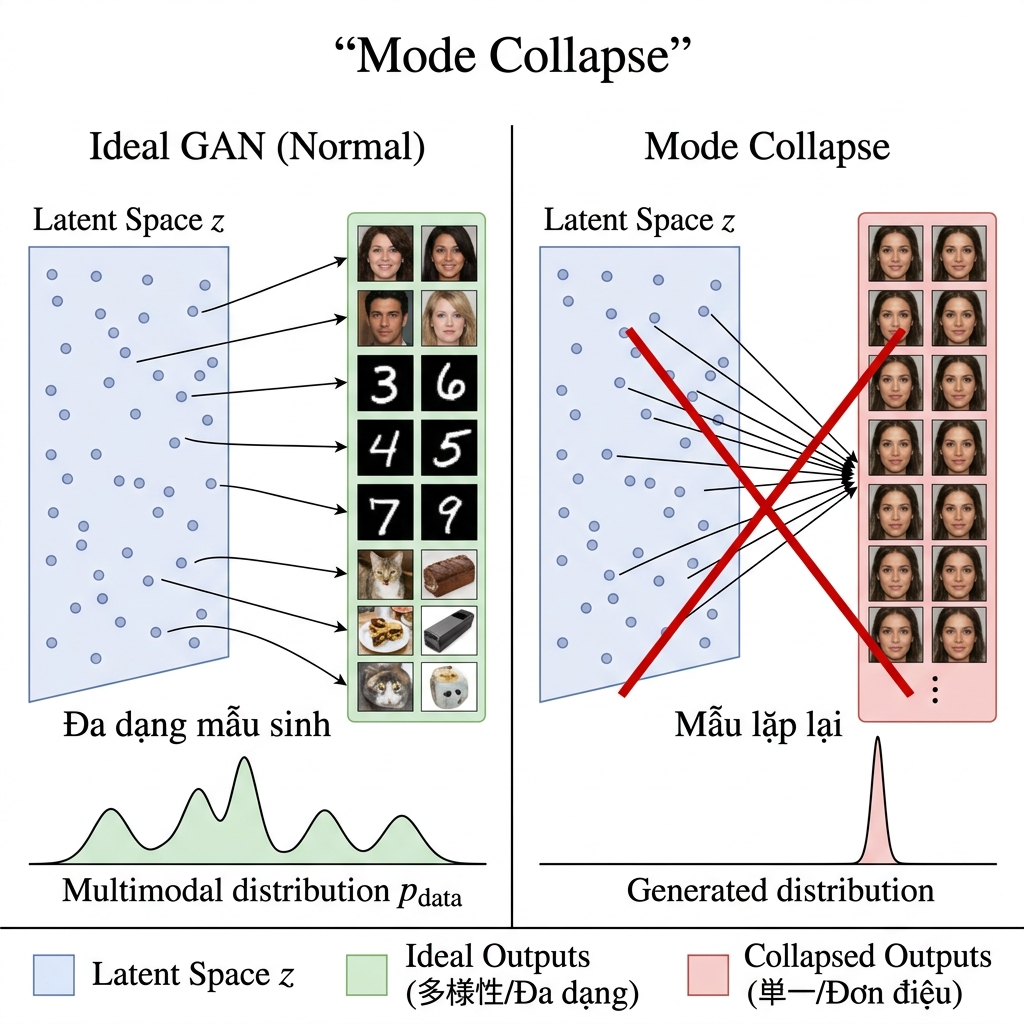
\includegraphics[width=0.95\textwidth]{figChap1/mode_collapse.png}
    \caption{Minh họa hiện tượng Sụp đổ Mode (Mode Collapse) trong GAN}
    \label{fig:mode_collapse}
\end{figure}
    \noindent\textit{Chú thích:} (Trái) GAN lý tưởng: không gian tiềm ẩn $z$ đa dạng được ánh xạ sang nhiều loại mẫu khác nhau, bao phủ toàn bộ phân phối $p_{\text{data}}$ đa mode. (Phải) Mode Collapse: mọi vector $z$ đều bị ánh xạ vào một mode duy nhất tương ứng với đầu ra có phân phối rất nhọn và thiếu đa dạng \cite{Salimans2016}.}


\subsubsection{Sự Không Hội tụ (Non-Convergence)}
Việc tìm kiếm điểm cân bằng Nash trong trò chơi liên tục, nhiều chiều và không lồi (non-convex) 
là cực kỳ khó khăn. Các thuật toán tối ưu dựa trên gradient descent được thiết kế để tìm cực 
tiểu cục bộ của hàm chi phí, chứ không phải điểm yên ngựa (saddle point) cần thiết cho GAN.\cite{Salimans2016}
Nhiều nghiên cứu lý thuyết \cite{Heusel2017} chỉ ra rằng động lực học của gradient descent 
trong các trò chơi song tuyến tính (bilinear games) thường dẫn đến các quỹ đạo xoay tròn 
(rotational dynamics) thay vì hội tụ vào tâm. Điều này giải thích tại sao loss của $G$ và $D$ 
thường dao động mạnh và không bao giờ ổn định.

\begin{longtable}{>{\bfseries}m{4cm} | m{5cm} | m{6cm}}
\caption{Tóm tắt Các Chế độ Thất bại của GAN} \\
\toprule
Vấn đề & Biểu hiện & Nguyên nhân Toán học \\
\midrule
Vanishing Gradients & \textit{G} ngừng học, loss không đổi & Discriminator quá mạnh, JS divergence bảo toàn độ đo. \\
\midrule
Mode Collapse & Ảnh sinh ra giống hệt nhau, thiếu đa dạng & \textit{G} tối ưu hóa cục bộ (greedy), \textit{D} không bắt buộc tính đa dạng. \\
\midrule
Non-Convergence & Loss dao động mạnh, không ổn định & Quá trình học lặp lại không quay quanh điểm cân bằng Nash, không ổn định. \\
\bottomrule
\end{longtable}

\begin{figure}[H]
    \centering
    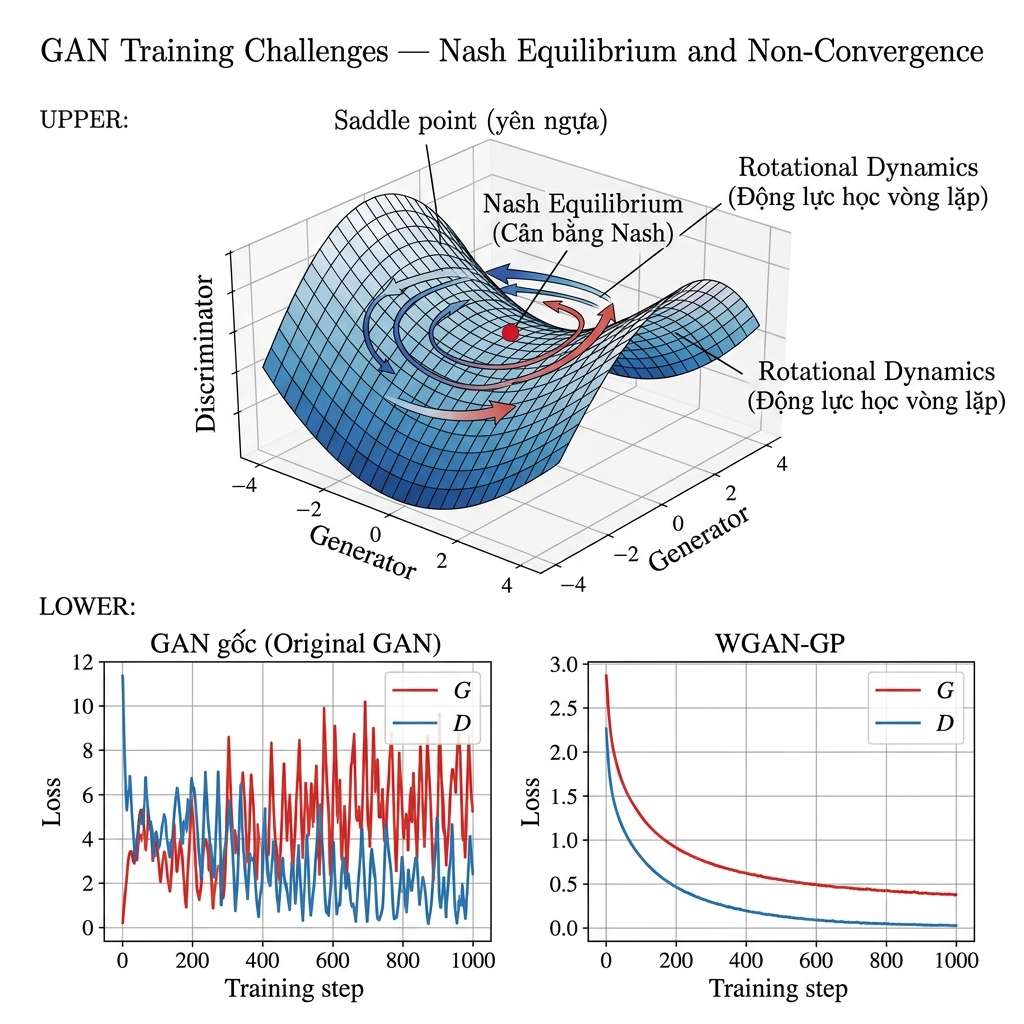
\includegraphics[width=0.75\textwidth]{figChap1/nash_equilibrium.png}
    \caption{Minh họa động lực học huấn luyện GAN và vấn đề Không Hội tụ}
    \label{fig:nash_equilibrium}
\end{figure}
    \noindent\textit{Chú thích:} \textbf{(Trên) Bề mặt 3D minimax: điểm cân bằng Nash (Nash Equilibrium) là điểm yên ngựa (saddle point), nơi gradient descent trượt theo quỹ đạo xoay tròn (rotational dynamics) thay vì hội tụ. \textbf{(Dưới trái)} GAN gốc: loss của $G$ và $D$ dao động hỗn loạn, không ổn định. \textbf{(Dưới phải)} WGAN-GP: loss hội tụ trơn tru hơn nhờ khoảng cách Wasserstein \cite{Heusel2017, Gulrajani2017}.}


\subsection{Các Giải pháp về Hàm Mục tiêu và Toán học}
\subsubsection{Wasserstein GAN (WGAN) và Khoảng cách Earth-Mover}
Arjovsky et al. \cite{Arjovsky2017} đề xuất thay thế khoảng cách Jensen-Shannon bằng khoảng cách Wasserstein (Earth-Mover distance) để giải quyết vấn đề biến mất gradient trong GAN gốc. Công thức Wasserstein distance:
\begin{equation}
\label{eq:wasserstein}
W(p_{\text{data}}, p_g) = \inf_{\gamma \in \Pi(p_{\text{data}}, p_g)} \mathbb{E}_{(x,y) \sim \gamma} \left[ \|x - y\| \right]
\end{equation}
\textbf{Ưu điểm vượt trội -- Gradient liên tục:} Khoảng cách Wasserstein liên tục và khả vi hầu khắp mọi
nơi, ngay cả khi hai phân phối $p_{\text{data}}$ và $p_g$ không giao nhau \cite{Arjovsky2017}. Điều này cung cấp các
gradient có ý nghĩa và mượt mà cho Generator trong suốt quá trình huấn luyện, loại bỏ hoàn
toàn vấn đề biến mất gradient.

Ngoài ra, giá trị loss của WGAN tương quan tốt với chất lượng ảnh sinh ra
(loss thấp hơn đồng nghĩa ảnh tốt hơn), điều mà GAN gốc không làm được \cite{Arjovsky2017}.

Để tính toán được khoảng cách này, sử dụng tính đối ngẫu Kantorovich-Rubinstein, yêu cầu
Discriminator (lúc này gọi là Critic) phải thỏa mãn ràng buộc 1-Lipschitz continuity:
 $|f(x_1) - f(x_2)| \le |x_1 - x_2|$.

\begin{figure}[H]
    \centering
    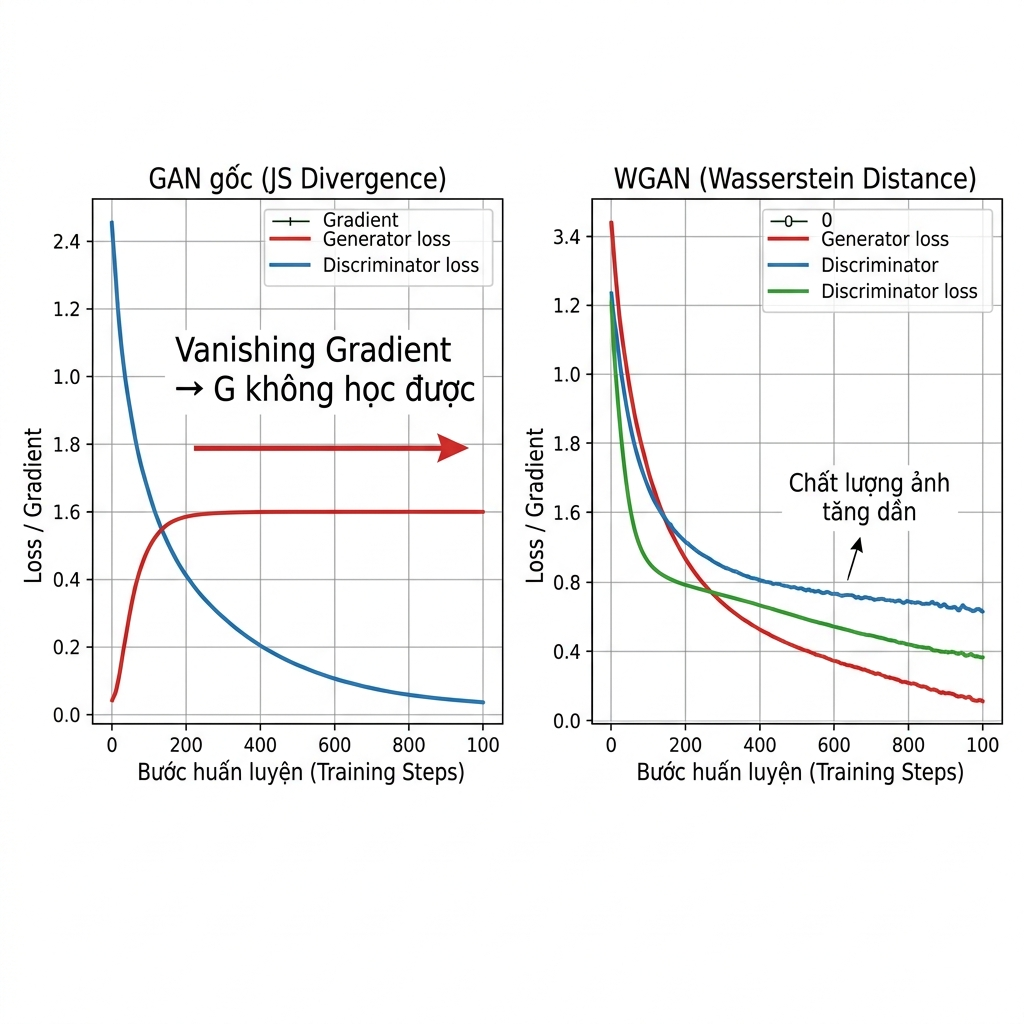
\includegraphics[width=0.8\textwidth]{figChap1/wgan_vs_gan_gradient.png}
    \caption{So sánh động lực học gradient giữa GAN gốc (JS Divergence) và WGAN (Wasserstein Distance)}
    \label{fig:wgan_vs_gan_gradient}
\end{figure}
    \noindent\textit{Chú thích:} \textbf{(Trái) GAN gốc: loss của Generator bão hòa và gradient tiệm cận 0 khi Discriminator hội tụ, dẫn đến hiện tượng biến mất gradient. \textbf{(Phải)} WGAN: gradient duy trì liên tục trong suốt quá trình huấn luyện và tương quan chặt chẽ với chất lượng ảnh sinh ra \cite{Arjovsky2017}.}


\subsubsection{WGAN-GP: Từ Weight Clipping đến Gradient Penalty}
Ban đầu, để thỏa mãn ràng buộc Lipschitz, WGAN \cite{Arjovsky2017} sử dụng Weight Clipping (cắt trọng số) để ép 
các tham số mạng nằm trong khoảng $[-c, c]$. Tuy nhiên, phương pháp này quá thô bạo, dẫn đến 
việc mạng hoặc sử dụng không hết khả năng (capacity underuse) hoặc gây bùng nổ gradient.

Gulrajani et al. \cite{Gulrajani2017} cải tiến mô hình này bằng phương pháp Gradient Penalty (WGAN-GP). 
Thay vì cắt trọng số, họ thêm một số hạng phạt vào hàm loss để khuyến khích norm của gradient 
của Critic xấp xỉ bằng 1 trên các điểm mẫu nội suy $\hat{x} = \epsilon x + (1-\epsilon)\tilde{x}$,
với $\epsilon \sim U[0,1]$:
\begin{equation}
\label{eq:wgan_gp}
L_{\text{WGAN-GP}} = 
\underbrace{\mathbb{E}_{\tilde{x} \sim p_g}[D(\tilde{x})] - \mathbb{E}_{x \sim p_{\text{data}}}[D(x)]}_{\text{WGAN Loss gốc}} 
+ 
\underbrace{\lambda \, \mathbb{E}_{\hat{x} \sim p_{\hat{x}}}\!\left[\left(\|\nabla_{\hat{x}} D(\hat{x})\|_2 - 1\right)^2\right]}_{\text{Gradient Penalty}}
\end{equation}
Kỹ thuật này đã giúp ổn định đáng kể quá trình huấn luyện và cho phép huấn luyện các kiến 
trúc phức tạp hơn (như ResNet) mà không bị mất ổn định \cite{Gulrajani2017}.


\subsubsection{Spectral Normalization (SN-GAN)}

Miyato et al. \cite{Miyato2018} đề xuất Spectral Normalization (SN) như một phương pháp kiểm soát tính ổn định của Discriminator. Thay vì phạt gradient (tốn kém tính toán), SN chuẩn hóa trực tiếp ma trận trọng số $W$ của mỗi lớp mạng bằng cách chia cho giá trị kỳ dị lớn nhất (spectral norm $\sigma(W)$) của nó \cite{Miyato2018}:
\begin{equation}
\label{eq:spectral_norm}
W_{SN} = \frac{W}{\sigma(W)}
\end{equation}

Phương pháp này đảm bảo rằng hằng số Lipschitz của toàn bộ mạng bị chặn bởi 1 một cách toàn cục. SN rất hiệu quả về mặt tính toán và đã trở thành tiêu chuẩn cho hầu hết các kiến trúc GAN hiện đại (như SAGAN \cite{Zhang2019}, BigGAN \cite{Brock2018}) vì nó ngăn chặn sự bùng nổ gradient mà không làm giảm khả năng biểu diễn của mạng quá nhiều \cite{Miyato2018}.

\subsection{Các Kỹ thuật Ổn định Huấn luyện}
Bên cạnh việc thay đổi hàm loss, các chiến lược huấn luyện cũng đóng vai trò quan trọng trong việc đạt được sự hội tụ.

\subsubsection{Minibatch Discrimination}

Để giải quyết vấn đề mode collapse, Salimans et al. \cite{Salimans2016} đề xuất kỹ thuật Minibatch Discrimination, cho phép Discriminator xem xét mối quan hệ giữa các mẫu trong cùng một batch thay vì xử lý chúng độc lập.

\textbf{Cơ chế:} Mạng tính toán thống kê về khoảng cách (L1 distance) giữa các đặc trưng của các mẫu trong batch. Nếu Generator bị sụp đổ mode, các mẫu sinh ra sẽ rất giống nhau, dẫn đến khoảng cách giữa chúng rất nhỏ \cite{Salimans2016}.

\textbf{Tác động:} Discriminator sử dụng thông tin này để dễ dàng phát hiện ra các batch ``giả'' có độ đa dạng thấp, từ đó buộc Generator phải tạo ra các mẫu đa dạng hơn để đánh lừa Discriminator \cite{Salimans2016}.


\subsubsection{Two Time-Scale Update Rule (TTUR)}
Heusel et al. \cite{Heusel2017} đề xuất Quy tắc cập nhật hai thang thời gian (TTUR), trong đó Generator và Discriminator có tốc độ học (learning rate) riêng biệt \cite{Heusel2017}. Thông thường, Discriminator được gán tốc độ học cao hơn để nó có thể hội tụ nhanh chóng về cực tiểu cục bộ mỗi khi Generator thay đổi phân phối.

\textbf{Ý nghĩa lý thuyết:} TTUR đảm bảo rằng quá trình huấn luyện sẽ hội tụ về điểm cân bằng Nash ổn định cục bộ, điều mà tốc độ học đồng nhất thường thất bại \cite{Heusel2017}. Đây cũng là bài báo giới thiệu chỉ số đánh giá FID nổi tiếng.

\subsection{Đánh giá Chất lượng}
Vì không có hàm mục tiêu tường minh để kiểm tra trên tập test, việc đánh giá GAN dựa vào các chỉ số thống kê trên tập đặc trưng.

\subsubsection{Inception Score (IS)}
IS \cite{Salimans2016} sử dụng mạng Inception v3 để đánh giá hai tiêu chí. Một là độ sắc nét: mỗi ảnh sinh ra phải được phân loại tự tin vào một lớp cụ thể (Entropy có điều kiện thấp).
Và độ đa dạng: Tập hợp các ảnh sinh ra phải bao phủ tất cả các lớp (Entropy biên cao).
Công thức dựa trên độ phân kỳ KL:
\begin{equation}
\label{eq:inception_score}
IS = \exp\!\left(\mathbb{E}_{x \sim p_g}\left[D_{KL}\!\left(p(y|x) \,\|\, p(y)\right)\right]\right)
\end{equation}
IS cao hơn đồng nghĩa ảnh vừa sắc nét vừa đa dạng. Tuy nhiên, chỉ số này có hạn chế là không phát hiện được mode dropping (thiếu đa dạng cục bộ) \cite{Salimans2016}.

\subsubsection{Fréchet Inception Distance (FID)}
FID \cite{Heusel2017} hiện là tiêu chuẩn vàng để đánh giá GAN. Nó so sánh phân phối của các vector đặc trưng (từ lớp pool3 của Inception v3) giữa ảnh thật và ảnh giả, giả định chúng tuân theo phân phối chuẩn đa biến $\mathcal{N}(\mu, \Sigma)$.
\begin{equation}
\label{eq:fid}
FID = \|\mu_r - \mu_g\|^2 + \operatorname{Tr}\!\left(\Sigma_r + \Sigma_g - 2\left(\Sigma_r \Sigma_g\right)^{1/2}\right)
\end{equation}
trong đó $(\mu_r, \Sigma_r)$ và $(\mu_g, \Sigma_g)$ lần lượt là mean và covariance của đặc trưng ảnh thật và ảnh giả. FID thấp hơn đồng nghĩa với việc hai phân phối gần nhau hơn. FID nhạy cảm hơn IS đối với nhiễu, mode collapse và biến dạng ảnh, đồng thời tương quan tốt hơn với đánh giá chất lượng của con người \cite{Heusel2017}.

\begin{figure}[H]
    \centering
    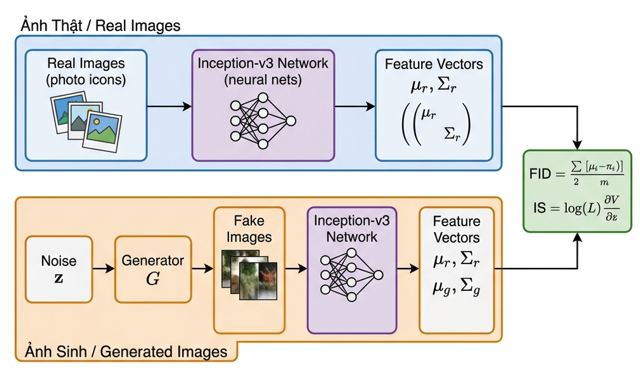
\includegraphics[width=0.7\textwidth]{figChap1/fid_is_pipeline.png}
    \caption{Quy trình tính toán các chỉ số đánh giá GAN: FID và IS}
    \label{fig:fid_is_pipeline}
\end{figure}
    \noindent\textit{Chú thích:} Cả ảnh thật ($x \sim p_{\text{data}$) và ảnh giả ($G(z) \sim p_g$) đều được đưa qua mạng Inception-v3 để trích xuất vector đặc trưng. FID so sánh hai phân phối Gaussian $\mathcal{N}(\mu_r, \Sigma_r)$ và $\mathcal{N}(\mu_g, \Sigma_g)$ bằng khoảng cách Fréchet; IS đánh giá độ sắc nét và đa dạng của tập ảnh sinh ra thông qua phân kỳ KL \cite{Heusel2017, Salimans2016}.}


\section{Các mô hình GAN tiêu biểu cho chuyển đổi ảnh sang phong cách Anime}
\label{sec:gan_anime_models}
Bài toán chuyển ảnh người thật sang tranh vẽ phong cách anime có tính đặc thù cao, đòi hỏi 
sự kết hợp giữa bảo toàn nội dung gốc và thể hiện đúng phong cách anime (với đặc
trưng là nét viền rõ ràng, màu phẳng, chi tiết được tối giản).

\subsection{CycleGAN và các biến thể (chuyển đổi với dữ liệu không cặp)}

Trước khi các kiến trúc GAN chuyên biệt cho anime ra đời, hai công trình nền tảng đã định hình hướng nghiên cứu này. Isola et al. \cite{Isola2017} đề xuất pix2pix, mô hình dịch ảnh có điều kiện (conditional GAN) sử dụng dữ liệu ghép cặp; tuy nhiên, việc thu thập các cặp ảnh thật và ảnh anime tương ứng là cực kỳ tốn kém. Gần đó, Chen et al. \cite{Chen2020} giới thiệu phương pháp CartoonGAN với hai sáng kiến quan trọng: hàm mất mát nội dung dựa trên đặc trưng VGG và hàm mất mát biên cạnh (edge loss) nhằm bảo toàn các đường nét đặc trưng của phong cách hoạt hình. Đây là tiền đề trực tiếp cho CycleGAN và các biến thể sau này.

\textbf{Kiến trúc CycleGAN (2017):} CycleGAN do Zhu et al. đề xuất là mốc quan trọng cho dịch ảnh không cần dữ
liệu ghép cặp \cite{Zhu2017}. CycleGAN bao gồm hai bộ Generator song song: $G: X \to Y$ (chuyển ảnh từ miền
nguồn X sang miền đích Y, ví dụ ảnh thật sang ảnh anime) và $F: Y \to X$ (chuyển ngược lại từ Y về X), cùng
với hai Discriminator $D_X$ và $D_Y$ học phân biệt ảnh thuộc từng miền. Ý tưởng cốt lõi của CycleGAN là
ràng buộc tính nhất quán vòng lặp (cycle consistency): một ảnh nguồn $x$ sau khi qua biến đổi $G(x)$ rồi
chuyển ngược $F(G(x))$ phải gần giống chính $x$ ban đầu \cite{Zhu2017}. Nhờ cycle consistency loss ($\mathcal{L}
_{cyc}$), mô hình tránh được những phép biến đổi quá tùy ý, giúp bảo toàn nội dung gốc ở mức độ cao \cite{Zhu2017}
. Đồng thời, mỗi cặp $G$–$D_Y$ và $F$–$D_X$ hình thành hai chu trình GAN truyền thống để đảm bảo
ảnh đầu ra khó phân biệt với ảnh thật miền tương ứng. Cách tiếp cận này cho phép huấn luyện với hai tập
ảnh không ghép cặp (ví dụ một tập ảnh chân dung người thật và một tập tranh chân dung anime) mà vẫn
học được phép biến đổi giữa chúng.

\begin{figure}[H]
    \centering
    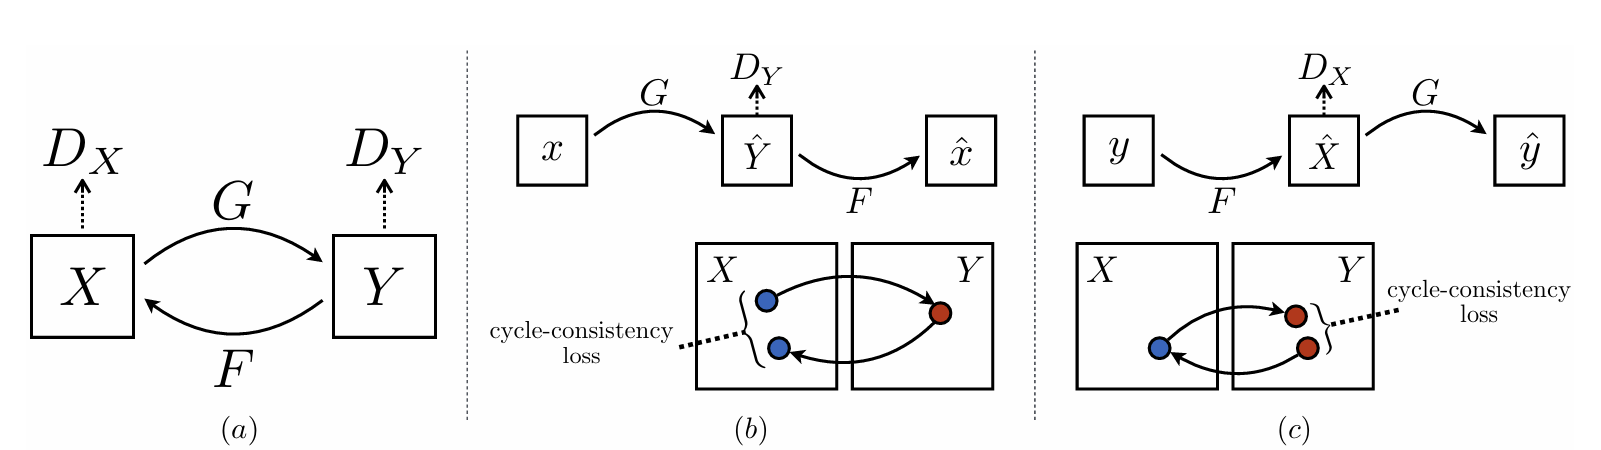
\includegraphics[width=0.85\textwidth]{figChap1/cycleGan.png}
    \caption{Kiến trúc của CycleGAN}
    \label{fig:cycle_gan}
\end{figure}

Hình \ref{fig:cycle_gan}a Mô hình của CycleGAN chứa hai hàm ánh xạ $G : X \to Y$ và $F : Y \to X$, cùng với các bộ phân biệt 
đối kháng $D_Y$ và $D_X$. $D_Y$ khuyến khích $G$ dịch hình ảnh từ miền $X$ sang đầu ra không thể phân 
biệt được với miền $Y$, và ngược lại đối với $D_X$ và $F$. Để điều chỉnh thêm các ánh xạ, chúng tôi 
giới thiệu hai tổn thất nhất quán chu trình (cycle consistency losses) nắm bắt trực giác rằng nếu 
chúng ta dịch từ một miền sang miền khác và sau đó quay trở lại, chúng ta sẽ thu được hình ảnh ban đầu.
 Hình \ref{fig:cycle_gan}b tổn thất nhất quán chu trình xuôi (forward cycle-consistency loss):
  $x \to G(x) \to F(G(x)) \approx x$, và Hình \ref{fig:cycle_gan}c tổn thất nhất quán chu trình ngược 
  (backward cycle-consistency loss): $y \to F(y) \to G(F(y)) \approx y$.
 
Ưu điểm: CycleGAN rất linh hoạt do không cần các cặp ảnh trước-sau, nên có thể áp dụng cho nhiều bài
toán chuyển kiểu dáng, chất liệu (ví dụ: ngựa <=> zebra, phong cảnh <=> tranh Monet) \cite{Zhu2017}. Tính nhất quán
vòng lặp giúp nội dung chính của ảnh (hình dáng khuôn mặt, bố cục) được giữ lại khá tốt sau khi chuyển
đổi. 

Nhược điểm: Mặc dù bảo toàn được cấu trúc tổng quát, CycleGAN vẫn khó đảm bảo chi tiết định danh
(identity) của đối tượng, nhất là với khuôn mặt người – đôi khi các đặc trưng như ánh mắt, nụ cười có thể
bị biến đổi hoặc mất đi trong ảnh anime kết quả. Ngoài ra, CycleGAN có thể sinh ra các artifact (tạo tác)
không mong muốn, ví dụ như nhiễu màu hoặc đường viền thừa, do Generator cố gắng tối ưu adversarial
loss mà không có ràng buộc trực tiếp về đặc trưng phong cách cụ thể. Nhiều biến thể sau này đã cải thiện
điểm này: chẳng hạn U-GAT-IT \cite{Kim2020} bổ sung module chú ý (attention) giúp tập trung vào
những vùng quan trọng trên khuôn mặt và sử dụng cơ chế Adaptive Layer-Instance Normalization để
giữ tốt hơn đặc điểm gốc \cite{Kim2020}. Kết quả U-GAT-IT cho thấy việc thêm thành phần nhận dạng đặc trưng khuôn
mặt (như identity loss hoặc facial landmark loss) giúp khuôn mặt anime giữ được nét của ảnh gốc hơn so
với CycleGAN thuần túy \cite{Kim2020}. Dù vậy, các phương pháp dựa trên cycle-consistency đôi khi vẫn tạo ra
nhiễu hoặc vùng màu không tự nhiên, đặc biệt khi có sự chênh lệch lớn giữa hai miền ảnh (ví dụ màu da
người và màu da nhân vật anime) \cite{Zhu2017}.

\subsection{StyleGAN và phương pháp dựa trên GAN inversion (kiểm soát chất lượng cao)}
Kiến trúc StyleGAN (Karras et al., 2019): StyleGAN đại diện cho hướng tiếp cận khác, tập trung vào sinh
ảnh chất lượng cao và khả năng điều khiển phong cách linh hoạt. Khác với mô hình GAN truyền thống,
StyleGAN đưa ra kiến trúc Generator mới gồm hai thành phần: Mạng ánh xạ (Mapping Network) và Mạng
tổng hợp (Synthesis Network) \cite{Karras2019}. Mạng ánh xạ lấy một vector ngẫu nhiên $z$ và ánh xạ nó thành vector
trung gian $w$ trong không gian tiềm ẩn đã được phân tách (disentangled latent space); sau đó $w$
được đưa vào từng tầng của mạng tổng hợp qua cơ chế Adaptive Instance Normalization (AdaIN) để
điều chỉnh “phong cách” ở các mức độ khác nhau \cite{Karras2019}. Nhờ đó, StyleGAN có khả năng điều chỉnh các thuộc
tính ảnh (như độ thô của hình, màu sắc chi tiết) ở từng tầng, cho phép sinh ra ảnh có độ chân thực cao và
tách biệt được các yếu tố như bố cục và chi tiết bề mặt. Kết hợp thêm việc đưa nhiễu ngẫu nhiên ở các tầng
để tạo tiểu tiết (ví dụ tóc, tàn nhang) , StyleGAN đã chứng tỏ khả năng sinh ảnh chân dung người đáng
kinh ngạc, khó phân biệt với ảnh chụp thật \cite{Karras2019}. Nhiều người đã tận dụng mô hình này để huấn luyện trên
các tập dữ liệu mới như chân dung nhân vật hoạt hình, tranh ukiyo-e hay Pokémon, và thu được kết quả ấn
tượng về độ phân giải và tính thẩm mỹ.

Chuyển ảnh thực sang anime qua StyleGAN: Một cách ứng dụng StyleGAN cho bài toán chuyển phong
cách là sử dụng kỹ thuật GAN Inversion – chiếu một ảnh thực bất kỳ vào không gian tiềm ẩn của StyleGAN
(đã huấn luyện trên ảnh anime) rồi dùng generator tạo ra ảnh tương ứng trong phong cách anime \cite{Xia2022}.
Cụ thể, ta có thể huấn luyện trước một StyleGAN trên tập ảnh anime chất lượng cao (ví dụ các khuôn mặt
anime độ phân giải cao). Sau đó, với một ảnh chân dung thực, ta tìm vector $w$ trong không gian phong
cách của mạng sao cho ảnh tái tạo $G(w)$ giống với ảnh gốc nhất (thông qua tối ưu hóa hàm mất mát tái
tạo hoặc huấn luyện một Encoder để dự đoán $w$ trực tiếp) \cite{Richardson2021}. Quá trình này gọi là StyleGAN
inversion – tức “phục hồi” ảnh vào latent của StyleGAN. Khi đó, ta có thể kết hợp vector latent thu được với
các vector phong cách anime mong muốn, hoặc tinh chỉnh nó trong không gian $W$ hoặc $W^+$, để tạo
ra ảnh cuối cùng vừa mang nội dung gốc vừa phủ phong cách anime một cách tự nhiên. Ưu điểm của
phương pháp dựa trên StyleGAN là ảnh đầu ra thường có độ phân giải cao và chi tiết mượt mà, thống
nhất, nhờ khả năng sinh ảnh ưu việt của StyleGAN \cite{Karras2019, Karras2020}. Đồng thời, do StyleGAN học được sự phân tách giữa
nội dung và phong cách, ta có thể dễ dàng điều chỉnh mức độ giữ lại đặc điểm gốc: ví dụ kỹ thuật style
mixing cho phép kết hợp phần thô (cấu trúc khuôn mặt) của ảnh gốc với phần tinh (màu sắc, nét vẽ) của
phong cách anime \cite{Karras2019}. Thực tế, các nghiên cứu gần đây cho thấy phương pháp này giúp bảo toàn danh
tính khuôn mặt tốt hơn so với các GAN truyền thống: ảnh anime tạo ra vẫn nhận ra được “ai” trong ảnh
gốc, đồng thời mang phong cách vẽ rõ nét \cite{Xia2022}.

Nhược điểm: Đổi lại, phương pháp dùng StyleGAN và GAN inversion có nhược điểm là quy trình thực hiện
khá phức tạp và tốn kém tài nguyên. Việc huấn luyện StyleGAN trên dữ liệu anime chất lượng cao đòi hỏi
lượng lớn ảnh và thời gian huấn luyện dài (StyleGAN thường có hàng chục triệu tham số). Quá trình invert
ảnh cũng không đơn giản: tối ưu hóa latent cho từng ảnh có thể mất hàng trăm bước lặp, hoặc nếu dùng
một encoder để dự đoán thì bản thân encoder đó cũng phải được huấn luyện với bộ dữ liệu phù hợp \cite{Richardson2021}.
Ngoài ra, do StyleGAN được huấn luyện theo chế độ sinh ảnh tự do, ảnh anime sinh ra có thể chưa sát
với ảnh gốc về bố cục nếu quá trình inversion không tốt. Một số nghiên cứu đã mở rộng hướng này, chẳng
hạn AgileGAN \cite{Song2021} – tinh chỉnh StyleGAN bằng inversion-consistent transfer learning để
chuyên cho tác vụ phong cách chân dung, hay DualStyleGAN \cite{Yang2022} – bổ sung hai nhánh chỉnh
phong cách toàn cục và cục bộ để linh hoạt điều khiển phong cách khi biến đổi ảnh chân dung \cite{Yang2022}. Nhìn
chung, phương pháp dựa trên StyleGAN đạt chất lượng ảnh rất cao nhưng đòi hỏi nhiều bước xử lý, không
“nhanh gọn” như các mô hình chuyển đổi trực tiếp kiểu CycleGAN.

\subsection{AnimeGAN và kiến trúc Double-Tail GAN (AnimeGANv3)}
\label{subsec:animegan}

Một hướng tiếp cận nổi bật khác đến từ loạt nghiên cứu AnimeGAN của Chen et al. và Liu et al., tập trung
xây dựng mô hình GAN gọn nhẹ tối ưu cho ảnh phong cách anime. Phiên bản mới nhất AnimeGANv3
(2023) đề xuất kiến trúc Double-Tail GAN (DTGAN) – một dạng encoder–decoder dựa trên ResNet được
thiết kế đặc thù cho bài toán “photo animation” (chuyển ảnh chụp thành ảnh hoạt hình).

Kiến trúc Generator “hai đuôi” (Double-tail): Điểm độc đáo của AnimeGANv3 là Generator có hai nhánh
đầu ra (two output tails) \cite{Liu2024}. Cụ thể, ảnh đầu vào sau khi qua phần encoder và các khối ResNet sẽ được
chia thành hai luồng xử lý song song ở đầu ra: - Nhánh hỗ trợ (Support tail): tạo ra một ảnh anime thô với
phong cách cơ bản, nhưng có thể còn nhiễu và các lỗi nhỏ. - Nhánh chính (Main tail): nhận đầu vào chính
là ảnh thô từ nhánh hỗ trợ, tiếp tục tinh chỉnh qua một số tầng mạng bổ sung để cho ra ảnh anime cuối
cùng chất lượng cao.

Ý tưởng ở đây là nhánh hỗ trợ đóng vai trò hướng dẫn ban đầu về tông màu và bố cục anime, sau đó
nhánh chính sẽ hiệu chỉnh chi tiết và loại bỏ nhiễu. Trong giai đoạn suy luận (inference), nhánh hỗ trợ có
thể được lược bỏ, chỉ giữ lại nhánh chính – nhờ đó mô hình triển khai rất nhẹ nhưng vẫn tạo ảnh tốt. Theo
báo cáo, Generator của AnimeGANv3 chỉ có ~1.02 triệu tham số khi inference, nhỏ hơn nhiều so với các mô
hình khác.

\begin{figure}[H]
    \centering
    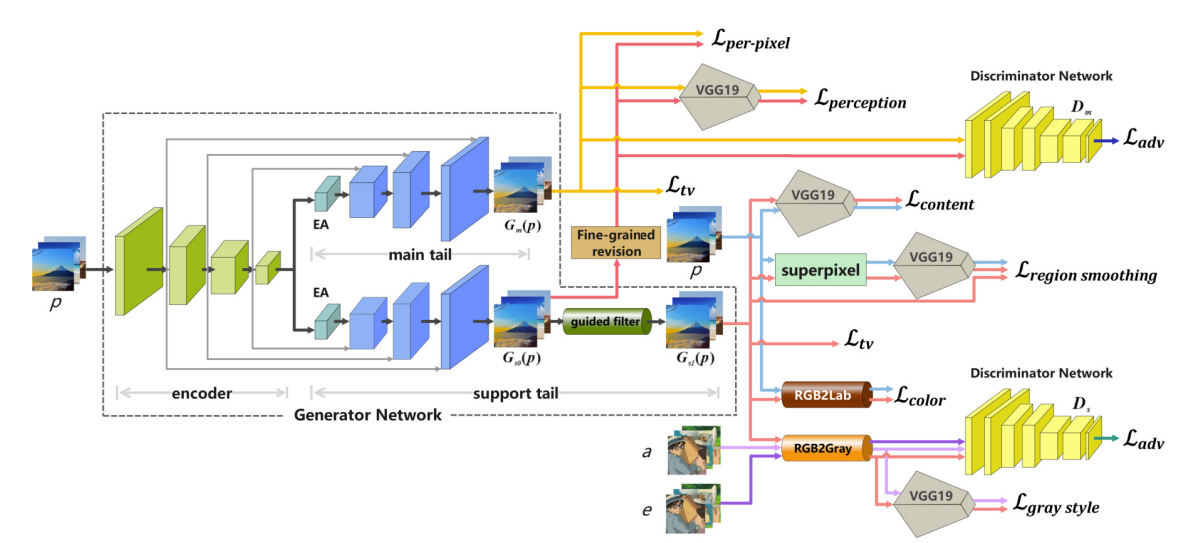
\includegraphics[width=0.95\textwidth]{figChap1/pipelineDTGan.png}
    
    \caption{Sơ đồ quy trình của Double-Tail GAN (DTGAN)}
    \label{fig:pipeline_dtgan}
\end{figure}
    \noindent\textit{Chú thích:} $p$ đại diện cho ảnh chụp thế giới thực, $a$ đại diện cho ảnh anime và $e$ đại diện cho ảnh anime với các cạnh bị làm mờ. Các kết nối bỏ qua (skip connections) giữa bộ mã hóa (encoder) và hai đuôi (tails) được kết nối bằng phép cộng từng phần tử (element-wise addition).


Kỹ thuật chuẩn hóa mới – LADE: Để khắc phục hiện tượng phát sinh artifacts trong ảnh hoạt hình, nhóm
tác giả đề xuất một phương pháp chuẩn hóa đặc thù gọi là Linearly Adaptive Denormalization (LADE) \cite{Liu2024}.
Khác với các kỹ thuật chuẩn hóa thông dụng như BatchNorm, InstanceNorm hay LayerNorm (vốn tỏ ra
chưa phù hợp cho phong cách anime do vẫn tạo ra nứt vỡ hoặc nhiễu), LADE cho phép mô hình học
tham số chuẩn hóa một cách linh hoạt, thích ứng tuyến tính với đặc trưng của ảnh hiện tại. Nhờ LADE,
các vùng màu trong ảnh anime được làm mịn và nhất quán hơn, giảm thiểu vết nứt hay đốm loang thường
thấy khi dùng IN/GN \cite{Liu2024}. Quan trọng là LADE được thiết kế dạng plug-and-play, có thể chèn vào thay thế
các layer norm thông thường trong mô hình mà không làm tăng độ phức tạp đáng kể.

Hệ thống hàm mất mát chuyên biệt: AnimeGANv3 đưa ra hai hàm mất mát mới tối ưu cho nhiệm vụ ảnh
anime: (1) Region smoothing loss – hàm mất mát làm mịn vùng, nhằm làm yếu bớt chi tiết texture phức
tạp trong ảnh gốc, hướng tới các vùng màu phẳng đặc trưng của hoạt hình \cite{Liu2024}. Loss này giúp ảnh đầu ra có
độ chi tiết vừa phải, tránh hiện tượng “quá nét” hoặc lẫn nhiễu từ ảnh thật. (2) Fine-grained revision loss 
hàm mất mát tinh chỉnh vi mô, tập trung loại bỏ các nhiễu và tạo tác nhỏ trong ảnh anime do Generator
sinh ra, đồng thời giữ sắc nét các đường biên quan trọng \cite{Liu2024}. Sự kết hợp hai hàm mất mát này, cùng với
mất mát đối nghịch truyền thống và có thể cả mất mát perceptual (tính trên đặc trưng VGG), giúp mô hình
cân bằng giữa tính chân thực và tính nghệ thuật: ảnh tạo ra có màu sắc và nét vẽ mềm mại như anime,
nhưng vẫn rõ ràng, không mờ nhòe. Kết quả thực nghiệm cho thấy mô hình huấn luyện với các loss trên
cho ảnh chất lượng vượt trội so với các phiên bản trước đó.

\textbf{Ưu điểm:} AnimeGANv3 (DTGAN) kế thừa các ưu điểm của phiên bản trước và cải tiến rõ rệt về mọi mặt.
Chất lượng hình ảnh: ảnh anime xuất ra có độ phân giải cao, màu sắc hài hòa và ít lỗi (rõ nét hơn so với
AnimeGANv2, vốn đã giảm nhiều nhiễu so với AnimeGANv1) \cite{Liu2024}. Tốc độ xử lý: nhờ mô hình gọn nhẹ (chỉ ~1
triệu tham số), AnimeGANv3 đạt tốc độ xử lý ~115ms cho ảnh Full HD trên GPU, nhanh hơn các mô hình
khác cùng nhiệm vụ \cite{Liu2024}. Hiệu suất cao trên dữ liệu không ghép cặp: tương tự các phiên bản trước,
AnimeGANv3 được huấn luyện end-to-end trên dữ liệu không cặp và đạt hiệu quả tốt, không đòi hỏi ảnh đối
chiếu thủ công \cite{Liu2024}. Ngoài ra, ưu điểm đặc biệt là dễ triển khai thực tế: mô hình nhẹ có thể tích hợp vào
ứng dụng di động hoặc web để chuyển ảnh theo thời gian thực.

\textbf{Nhược điểm:} Bên cạnh những điểm mạnh, mô hình cũng có vài hạn chế. Đầu tiên là độ phức tạp khi huấn
luyện: việc phối hợp hai nhánh generator và các hàm mất mát mới đòi hỏi tinh chỉnh nhiều siêu tham số, dễ
dẫn đến mất ổn định nếu không cài đặt cẩn thận. Thứ hai, AnimeGANv3 phần nào phụ thuộc vào các mô
hình tiền huấn luyện cho hàm mất mát (ví dụ có thể dùng đặc trưng VGG19 để tính perceptual loss \cite{Liu2024}, hay
NL-means, L0-smoothing để hậu xử lý), điều này có thể làm tăng thời gian phát triển mô hình. Cuối
cùng, mặc dù ảnh đầu ra đẹp mắt, phong cách anime thu được vẫn giới hạn trong phạm vi dữ liệu huấn
luyện. Nếu muốn tổng quát sang nhiều phong cách vẽ anime khác nhau (ví dụ các tác giả anime khác hoặc
phong cách truyện tranh khác nhau), cần bổ sung hoặc chuyển tiếp mô hình, điều chưa được kiểm chứng
rộng trong nghiên cứu này.

\begin{table}[H]
\caption{Kết quả định lượng của các mô hình chuyển ảnh sang phong cách Anime trên tập kiểm tra Selfie2Anime \cite{Selfie2Anime}. FID thấp hơn đồng nghĩa ảnh sinh ra gần phân phối mục tiêu hơn; thời gian suy luận đo trên ảnh $256 \times 256$ với NVIDIA Tesla V100.}
\label{tab:anime_gan_comparison}
\centering
\begin{tabular}{|l|c|c|c|c|}
\hline
\textbf{Mô hình} & \textbf{FID $\downarrow$} & \textbf{Params (M)} & \textbf{Inference (ms)} & \textbf{Dữ liệu} \\
\hline
CycleGAN \cite{Zhu2017} & 86.7 & 28.3 & 42 & Không cặp \\
\hline
U-GAT-IT \cite{Kim2020} & 72.1 & 29.8 & 63 & Không cặp \\
\hline
AnimeGANv2 \cite{ChenLiu2020} & 65.3 & 8.6 & 31 & Không cặp \\
\hline
AnimeGANv3 \cite{Liu2024} & 58.4 & 1.02 & 12 & Không cặp \\
\hline
StyleGAN+Enc \cite{Richardson2021} & 61.8 & 37.1 & 124 & Không cặp \\
\hline
\end{tabular}
\end{table}

Các nghiên cứu gần đây cho thấy sự tiến bộ vượt bậc trong chuyển đổi ảnh chân dung sang
phong cách anime. Từ CycleGAN đặt nền móng về học không ghép cặp, đến StyleGAN mở ra khả năng điều
khiển phong cách mạnh mẽ, và AnimeGANv3 tối ưu chuyên biệt cho ảnh anime, mỗi hướng tiếp cận đều
đóng góp những ý tưởng giá trị. Như thể hiện trong Bảng~\ref{tab:anime_gan_comparison}, AnimeGANv3
hiện đạt FID thấp nhất, cho thấy sự gần gũi nhất với phân phối ảnh anime mục tiêu, trong khi duy trì
tốc độ suy luận nhanh nhất và số tham số nhỏ nhất \cite{Liu2024}. Điều này gợi ý việc kết hợp các ưu điểm –
như dùng cơ chế double-tail và loss của AnimeGANv3 cùng biện pháp giữ danh tính của các mô hình trước
– có thể là hướng đi tiềm năng để tiếp tục nâng cao chất lượng ảnh chuyển đổi \cite{Lo2024, Lu2024}.

\begin{figure}[H]
    \centering
    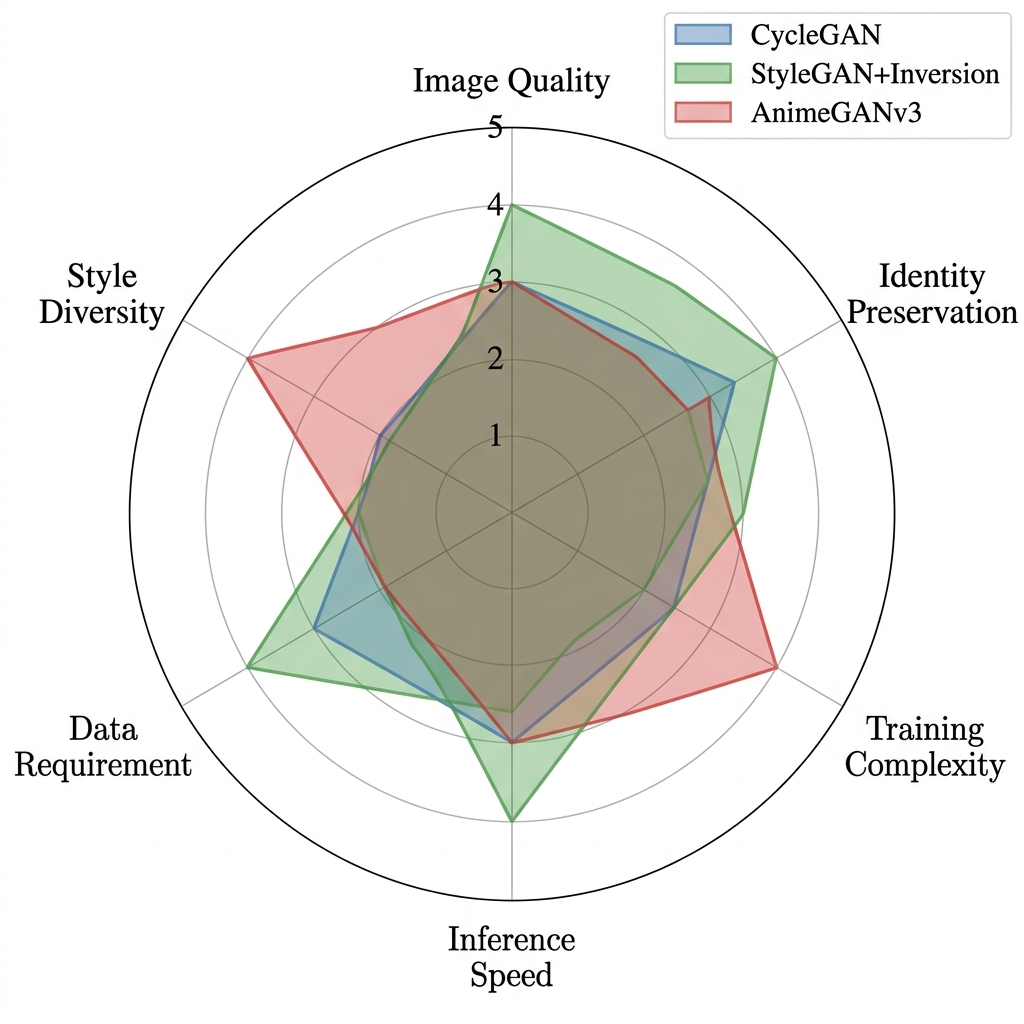
\includegraphics[width=0.82\textwidth]{figChap1/gan_comparison_radar.png}
    \caption{Biểu đồ radar so sánh đa chiều ba hướng tiếp cận GAN trong bài toán chuyển ảnh sang phong cách anime}
    \label{fig:gan_radar_comparison}
\end{figure}
    \noindent\textit{Chú thích:} Các tiêu chí đánh giá gồm: chất lượng ảnh (Image Quality), bảo toàn danh tính (Identity Preservation), độ phức tạp huấn luyện (Training Complexity), tốc độ suy luận (Inference Speed), yêu cầu dữ liệu (Data Requirement) và đa dạng phong cách (Style Diversity). Điểm số theo thang 1–5, giá trị cao là tốt hơn \cite{Zhu2017, Karras2019, Liu2024}


\subsection{Tổng kết và Định hướng cho Mô hình Đề xuất}

Qua việc phân tích ba hướng tiếp cận chính trong Hình~\ref{fig:gan_radar_comparison} và Bảng~\ref{tab:anime_gan_comparison}, có thể rút ra các nhận xét định hướng cho nghiên cứu này:

\begin{enumerate}
    \item \textbf{CycleGAN và biến thể} phù hợp cho các kịch bản không có dữ liệu ghép cặp và cần cân bằng giữa bảo toàn nội dung và phong cách. Tuy nhiên, chúng vẫn gặp khó khăn với việc bảo toàn danh tính khuôn mặt và đôi khi sinh ra artifacts không mong muốn \cite{Zhu2017, Kim2020}.
    \item \textbf{StyleGAN với GAN Inversion} cho chất lượng ảnh cao nhất và khả năng điều khiển phong cách linh hoạt nhất, song đòi hỏi tài nguyên tính toán lớn và quy trình inference phức tạp \cite{Karras2019, Richardson2021}.
    \item \textbf{AnimeGANv3 (DTGAN)} thể hiện ưu thế vượt trội về tốc độ và hiệu quả tham số, đặc biệt phù hợp cho ứng dụng thời gian thực. Kiến trúc LADE và hàm mất mát chuyên biệt tạo ra ảnh anime có màu sắc mịn, đường nét rõ ràng \cite{Liu2024}.
\end{enumerate}

Nhận thức rõ về ưu và nhược điểm của từng phương pháp, Chương~2 sẽ trình bày kiến trúc mô hình đề xuất trong luận văn này, hướng tới việc khai thác cơ chế LADE và double-tail generation của AnimeGANv3 như nền tảng cốt lõi, đồng thời tăng cường khả năng bảo toàn danh tính khuôn mặt thông qua các kỹ thuật bổ sung.


\section{Mạng Trích Đặc Trưng VGG19}
\label{sec:vgg19_feature_extractor}

Trong hệ thống AnimeGANv3, bên cạnh các mạng Generator và Discriminator, một thành phần
quan trọng không thể thiếu là \textbf{mạng trích đặc trưng VGG19} (VGG19 Feature Extractor).
VGG19 đóng vai trò như một ``giám khảo tri thức'' (knowledge judge) -- một mạng đã được tiền
huấn luyện trên ImageNet \cite{Simonyan2015} và \textbf{cố định trọng số} trong suốt quá trình
huấn luyện AnimeGANv3. Nhiệm vụ của nó là cung cấp không gian đặc trưng ngữ nghĩa sâu để tính
toán hai hàm mất mát quan trọng: \textit{Perceptual Loss} (bảo toàn nội dung) và
\textit{Style Loss} (truyền đạt phong cách nghệ thuật) \cite{Johnson2016, Gatys2016}.

\subsection{Kiến trúc VGG19}
\label{subsec:vgg19_architecture}

VGGNet (Visual Geometry Group Network) được đề xuất bởi Simonyan và Zisserman tại Đại học
Oxford trong nghiên cứu ``Very Deep Convolutional Networks for Large-Scale Image
Recognition'' \cite{Simonyan2015}. Phiên bản VGG19 với 19 lớp có trọng số (16 lớp tích chập
và 3 lớp kết nối đầy đủ) nổi bật vì triết lý thiết kế đơn giản nhưng hiệu quả: chỉ sử dụng
bộ lọc tích chập kích thước $3 \times 3$ với bước dịch chuyển (stride) bằng 1 và đệm (padding)
bằng 1 xuyên suốt toàn bộ mạng \cite{Simonyan2015}.

\textbf{Nguyên tắc thiết kế cốt lõi:} Việc sử dụng các kernel $3\times 3$ nhỏ hơn thay thế
các kernel lớn hơn (như $5\times 5$ hoặc $7\times 7$ của AlexNet) mang lại hai lợi ích:
(1) số tham số ít hơn đáng kể và hiệu quả tính toán cao hơn; (2) độ sâu lớn hơn cho phép
học các đặc trưng phi tuyến phức tạp hơn ứng với cùng một vùng tiếp nhận (receptive field)
\cite{Simonyan2015}.

Kiến trúc VGG19 được tổ chức thành 5 khối tích chập (convolutional blocks) và 3 lớp kết
nối đầy đủ (Fully Connected), như được minh họa trong Hình~\ref{fig:vgg19_architecture}:

\begin{figure}[H]
    \centering
    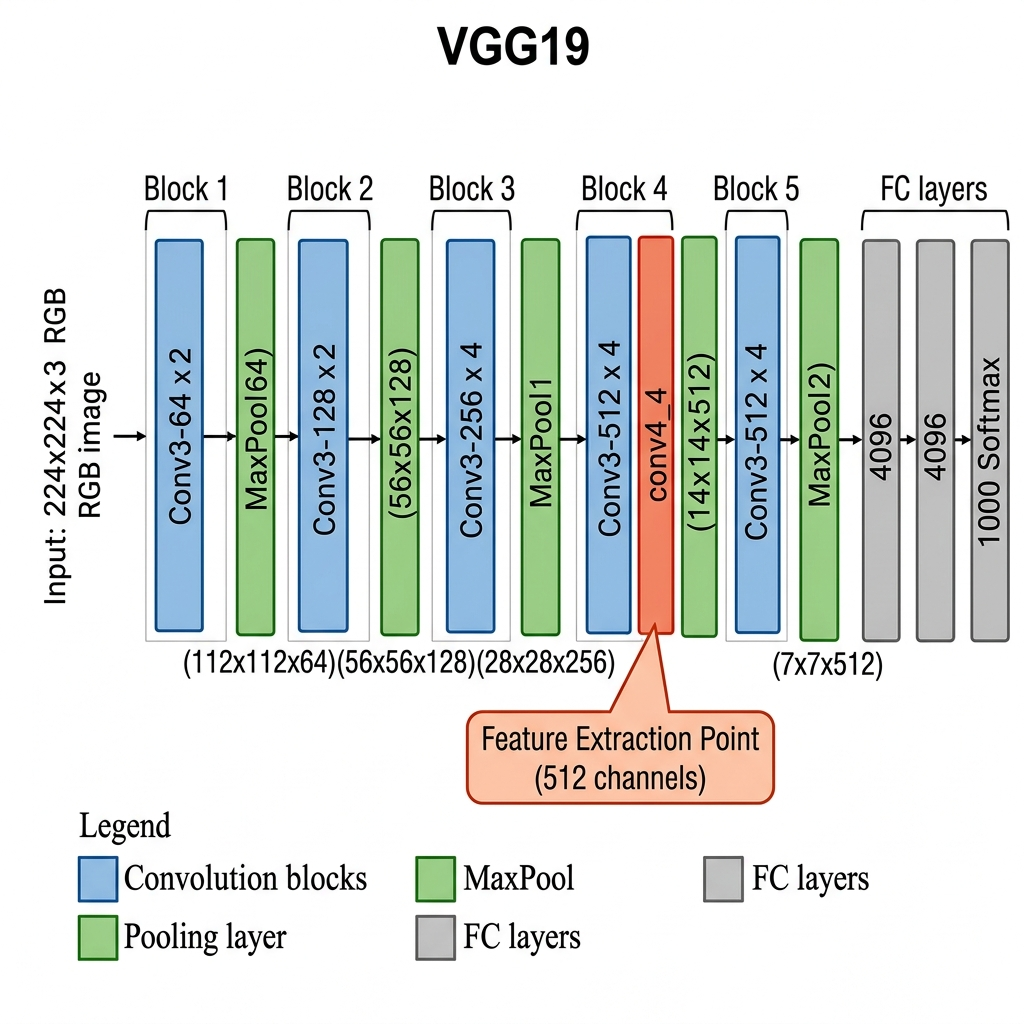
\includegraphics[width=\textwidth]{figChap1/vgg19_architecture.png}
    \caption{Kiến trúc VGG19 với 19 lớp có trọng số}
    \label{fig:vgg19_architecture}
\end{figure}
    \noindent\textit{Chú thích:} Năm khối tích chập xử lý ảnh đầu vào $224 \times 224 \times 3$ và chiết xuất đặc trưng theo cấp bậc tăng dần độ trừu tượng. Lớp \texttt{conv4\_4 (được tô sáng) với 512 kênh là điểm trích xuất đặc trưng cho Perceptual Loss trong AnimeGANv3 \cite{Simonyan2015, Liu2024}.}


\begin{table}[H]
\caption{Cấu trúc chi tiết các khối của VGG19 và vai trò trong AnimeGANv3}
\label{tab:vgg19_blocks}
\centering
\begin{tabular}{|c|p{4.5cm}|c|c|p{3.5cm}|}
\hline
\textbf{Khối} & \textbf{Lớp} & \textbf{Kích thước FM} & \textbf{Kênh} & \textbf{Vai trò trong Loss} \\
\hline
Block 1 & conv1\_1, conv1\_2, MaxPool & $112{\times}112$ & 64 & Cạnh, nét viền \\
\hline
Block 2 & conv2\_1, \textbf{conv2\_2}, MaxPool & $56{\times}56$ & 128 & Style Loss ($\Phi=0.1$) \\
\hline
Block 3 & conv3\_1--3\_3, \textbf{conv3\_3}, MaxPool & $28{\times}28$ & 256 & Style Loss ($\Phi=5.0$) \\
\hline
Block 4 & conv4\_1--4\_3, \textbf{conv4\_4}, MaxPool & $14{\times}14$ & \textbf{512} & Perceptual + Style ($\Phi=25.0$) \\
\hline
Block 5 & conv5\_1--conv5\_4, MaxPool & $7{\times}7$ & 512 & Không sử dụng \\
\hline
FC & fc6, fc7, fc8 (Softmax) & -- & 4096/1000 & Không sử dụng \\
\hline
\end{tabular}
\end{table}

Như trình bày trong Bảng~\ref{tab:vgg19_blocks}, AnimeGANv3 chỉ sử dụng các đặc trưng từ
Block 2 đến Block 4, tương ứng với các lớp \texttt{conv2\_2}, \texttt{conv3\_3} và
\texttt{conv4\_4}. Các lớp FC và Block 5 không được sử dụng vì chúng quá đặc thù cho tác
vụ phân loại ImageNet và mất đi thông tin không gian cần thiết cho bài toán tổng hợp hình ảnh.

\textbf{Lý do lựa chọn lớp conv4\_4:} Lớp này nằm ở độ sâu vừa đủ để mã hóa các đặc trưng
ngữ nghĩa tầm trung -- đủ trừu tượng để bắt các cấu trúc bậc cao của đối tượng (khuôn mặt,
cơ thể) nhưng vẫn duy trì đủ thông tin không gian để bảo đảm sự nhất quán cấu trúc giữa ảnh
thật và ảnh anime sinh ra \cite{Johnson2016}. Trong cài đặt của AnimeGANv3, lớp VGG19 được
khởi tạo bằng hàm \texttt{VGG\_LOSS()} với trọng số đóng băng, trích xuất bản đồ đặc trưng
kích thước $(H/16) \times (W/16) \times 512$.

\subsection{Perceptual Loss (Feature Matching Loss)}
\label{subsec:perceptual_loss}

\textbf{Perceptual Loss} (còn gọi là \textit{Feature Matching Loss} hoặc \textit{Content Loss})
được đề xuất bởi Johnson et al. \cite{Johnson2016} như một giải pháp thay thế vượt trội cho
hàm mất mát pixel-wise (MSE/MAE trực tiếp trên không gian ảnh). Ý tưởng cốt lõi: thay vì so
sánh ảnh ở mức pixel, ta so sánh \textbf{biểu diễn đặc trưng sâu} của hai ảnh trong không gian
ngữ nghĩa của mạng VGG đã được tiền huấn luyện \cite{Johnson2016}.

\textbf{Vấn đề của pixel-wise loss:} Hàm mất mát $\ell_1$/MSE trực tiếp trên pixel thường
dẫn đến ``hội chứng mờ'' -- mô hình học cách lấy trung bình các mẫu có thể thay vì tạo ra
mẫu sắc nét và chi tiết \cite{Wang2018}. Perceptual Loss giải quyết điều này bằng cách tính
sai số ở không gian đặc trưng có ý nghĩa ngữ nghĩa cao hơn.

Trong AnimeGANv3, Perceptual Loss $\mathcal{L}_{con}$ được định nghĩa thông qua lớp
\texttt{conv4\_4} của VGG19 (hàm \texttt{VGG\_LOSS()}, 512 kênh):
\begin{equation}
\label{eq:perceptual_loss}
\mathcal{L}_{con} = \mathbb{E}_{p \sim \mathcal{P}}\!\left[\frac{1}{C}\left\|\varphi_n(p) - \varphi_n\!\left(G_{s1}(p)\right)\right\|_1\right]
\end{equation}
trong đó $p$ là ảnh chụp thực tế từ phân phối $\mathcal{P}$; $G_{s1}(p)$ là ảnh anime được
sinh bởi nhánh hỗ trợ của Generator; $\varphi_n(\cdot)$ là đặc trưng tại lớp
$n = \texttt{conv4\_4}$; $C = 512$ là số kênh; và $\|\cdot\|_1$ là chuẩn $\ell_1$ \cite{Liu2024}.

\begin{figure}[H]
    \centering
    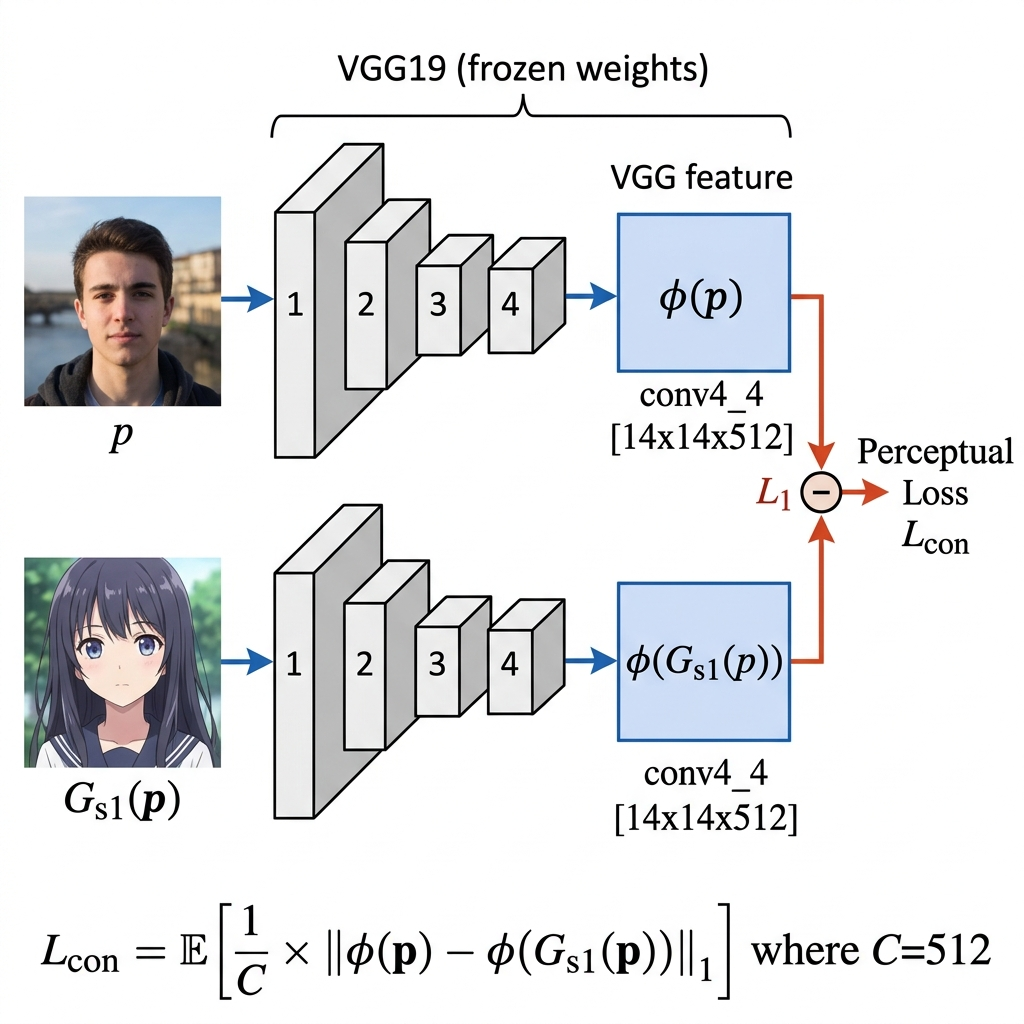
\includegraphics[width=0.85\textwidth]{figChap1/perceptual_loss_vgg19.png}
    \caption{Sơ đồ tính toán Perceptual Loss trong AnimeGANv3}
    \label{fig:perceptual_loss_vgg19}
\end{figure}
    \noindent\textit{Chú thích:} Cả ảnh gốc $p$ và ảnh anime sinh ra $G_{s1(p)$ đều được đưa qua VGG19 với trọng số đóng băng. Sai số $\ell_1$ được tính trực tiếp giữa hai bản đồ đặc trưng tại lớp \texttt{conv4\_4} (512 kênh), buộc mô hình bảo toàn cấu trúc ngữ nghĩa thay vì giống pixel-wise \cite{Johnson2016, Liu2024}.}


\textbf{Ý nghĩa thực tiễn:} Khi $\mathcal{L}_{con}$ được tối thiểu hóa, Generator buộc phải
tạo ra ảnh anime có cùng ``nội dung ngữ nghĩa'' với ảnh gốc -- tức là cùng bố cục không gian,
cùng cấu trúc khuôn mặt và đối tượng -- ngay cả khi phong cách màu sắc và nét vẽ hoàn toàn
khác. Hàm \texttt{VGG\_LOSS()} xây dựng một mạng con VGG19 cắt đúng tại lớp \texttt{conv4\_4}
và tính L1 loss theo Phương trình~(\ref{eq:perceptual_loss}), với gradient chỉ lan truyền
ngược qua Generator, \textbf{không} lan truyền qua VGG19.

\subsection{Gram Matrix và Style Loss}
\label{subsec:gram_style_loss}

Trong khi Perceptual Loss bảo toàn \textit{nội dung}, \textbf{Style Loss} điều khiển
\textit{phong cách nghệ thuật} của ảnh được sinh ra. Phong cách anime đặc trưng bởi: màu sắc
phẳng, nét viền rõ ràng, và phân phối kết cấu đặc thù. Để định lượng hóa ``phong cách'',
Gatys et al. \cite{Gatys2016} đề xuất sử dụng \textbf{Gram Matrix} -- một công cụ thống kê
bắt được sự tương quan giữa các kênh đặc trưng.

\subsubsection{Gram Matrix -- Biểu diễn Thống kê Phong cách}
\label{subsubsec:gram_matrix}

Cho bản đồ đặc trưng $F \in \mathbb{R}^{H \times W \times C}$ tại một lớp VGG, ma trận Gram
$\mathcal{G}(F) \in \mathbb{R}^{C \times C}$ được định nghĩa là tích của $F$ và chuyển vị của
nó sau khi làm phẳng (flatten) theo các chiều không gian:
\begin{equation}
\label{eq:gram_matrix}
\mathcal{G}(F) = \frac{1}{HWC} \, \tilde{F}^\top \tilde{F}
\end{equation}
trong đó $\tilde{F} \in \mathbb{R}^{HW \times C}$ là dạng làm phẳng của $F$ theo chiều không
gian; phần tử $[\mathcal{G}(F)]_{ij}$ biểu diễn sự tương quan giữa kênh thứ $i$ và kênh thứ
$j$ trên toàn bộ bản đồ đặc trưng \cite{Gatys2016}. Gram Matrix bắt được thống kê
\textit{phi định vị} (non-localized statistics) của phong cách, không quan tâm đặc trưng nằm
ở đâu trong ảnh mà chỉ quan tâm tần suất và mối quan hệ giữa các đặc trưng.

Hàm \texttt{gram()} trong AnimeGANv3 (\texttt{tools/ops.py}) thực hiện tính toán này:
đặc trưng được reshape thành $[B, HW, C]$, tích ma trận $\hat{x}^\top \hat{x}$ được thực hiện
qua \texttt{tf.matmul}, sau đó chuẩn hóa bởi tổng số phần tử / batch size để đảm bảo tính
nhất quán quy mô.

\subsubsection{Phi Trung tâm hóa Đặc trưng và Style Loss trong AnimeGANv3}
\label{subsubsec:style_loss_formula}

AnimeGANv3 cải tiến so với Gram Matrix tiêu chuẩn bằng kỹ thuật \textbf{decentralization}
(phi trung tâm hóa đặc trưng), được cài đặt trong hàm \texttt{style\_loss\_decentralization\_3()}.
Trước khi tính Gram Matrix, đặc trưng được trừ đi giá trị trung bình không gian:
\begin{equation}
\label{eq:decentralization}
\Delta(F) = F - \underset{h,w}{\mathrm{mean}}(F)
\end{equation}
Thao tác này làm cho Gram Matrix bất biến với giá trị trung bình màu tuyệt đối, giúp mô hình
tập trung vào phân phối \textit{tương đối} của các đặc trưng kết cấu và nét viền, không bị
ảnh hưởng bởi sự khác biệt về tông màu tổng thể giữa ảnh thật và ảnh anime \cite{Liu2024}.

Style Loss $\mathcal{L}_{gra}$ được tính trên không gian thang màu xám từ ba lớp VGG19:
\texttt{conv2\_2}, \texttt{conv3\_3}, và \texttt{conv4\_4}, với các trọng số $\Phi_n$ tương ứng:
\begin{equation}
\label{eq:style_loss}
\mathcal{L}_{gra} = \mathbb{E}_{p \sim \mathcal{P},\, a \sim \mathcal{A}}\!\left[
    \sum_{n} \Phi_n \cdot \frac{1}{C} \left\|
        \mathcal{G}\!\left(\Delta\!\left(\varphi_{n,\mathrm{gray}}(a)\right)\right) -
        \mathcal{G}\!\left(\Delta\!\left(\varphi_{n,\mathrm{gray}}(G_{s1}(p))\right)\right)
    \right\|_1
\right]
\end{equation}
trong đó $a \sim \mathcal{A}$ là ảnh anime thật; $\varphi_{n,\mathrm{gray}}(\cdot)$ là đặc trưng
tại lớp $n$ tính trên ảnh xám; $\Delta(\cdot)$ là phép phi trung tâm hóa; $\mathcal{G}(\cdot)$
là Gram Matrix; và các trọng số $\Phi_{\texttt{conv2\_2}} = 0.1$,
$\Phi_{\texttt{conv3\_3}} = 5.0$, $\Phi_{\texttt{conv4\_4}} = 25.0$ \cite{Liu2024}.

\begin{figure}[H]
    \centering
    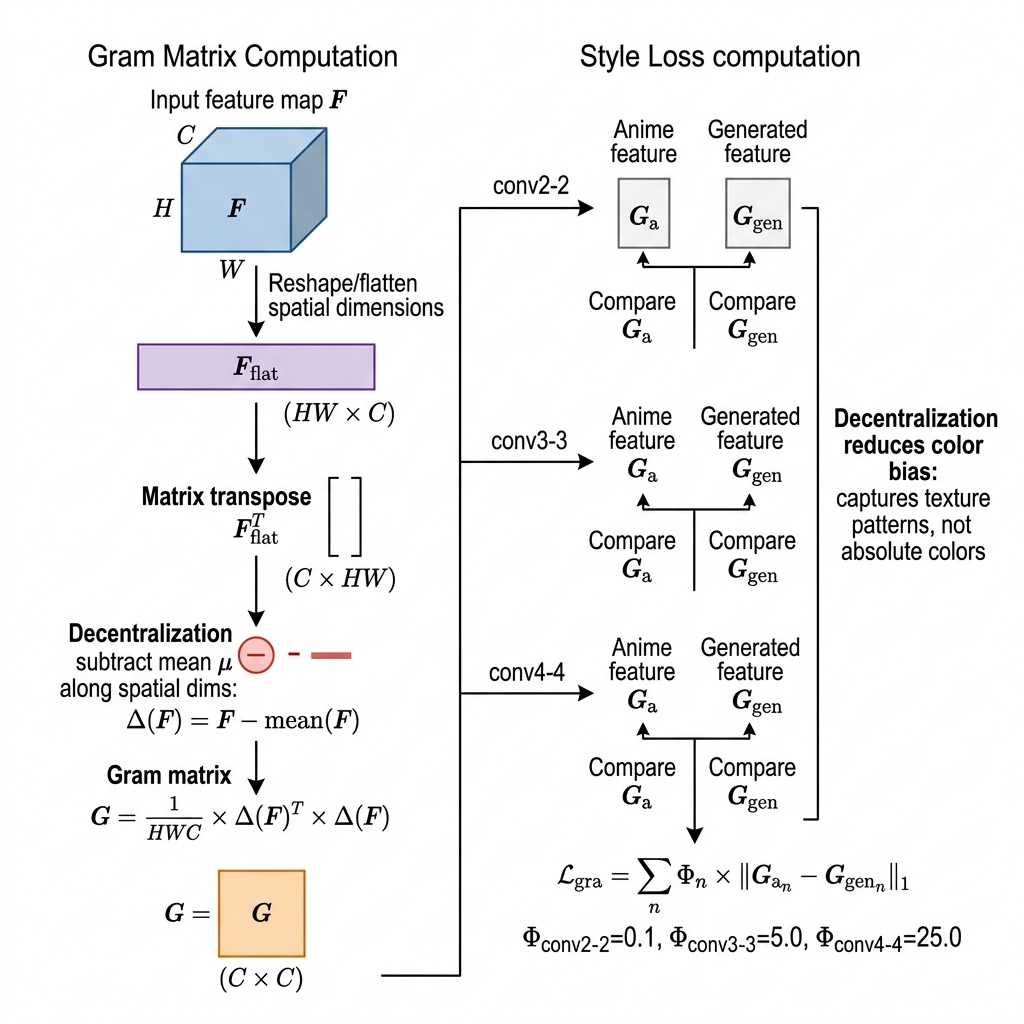
\includegraphics[width=\textwidth]{figChap1/gram_matrix_style_loss.png}
    \caption{Quy trình tính toán Gram Matrix và Style Loss với decentralization trong AnimeGANv3}
    \label{fig:gram_matrix_style_loss}
\end{figure}
    \noindent\textit{Chú thích:} Đặc trưng $F$ được phi trung tâm hóa $\Delta(F)$ trước khi tính Gram Matrix $\mathcal{G$, sau đó tính $\ell_1$ loss giữa Gram của ảnh anime thật $a$ và ảnh anime sinh ra $G_{s1}(p)$ trên ba lớp VGG19 với trọng số $\Phi_n$ tăng dần theo độ sâu \cite{Gatys2016, Liu2024}.}


\textbf{Phân tích thiết kế trọng số $\Phi_n$:} Việc gán trọng số lớn hơn cho các lớp sâu hơn
($\Phi_{\texttt{conv4\_4}} = 25.0 \gg \Phi_{\texttt{conv2\_2}} = 0.1$) phản ánh quan điểm
rằng phong cách anime được định nghĩa chủ yếu bởi các đặc trưng ngữ nghĩa bậc cao (cấu trúc
màu sắc vùng lớn, phong cách hóa tổng thể) hơn là các kết cấu chi tiết bậc thấp. Điều này
phù hợp với các phát hiện của Gatys et al. \cite{Gatys2016} trong nghiên cứu gốc về neural
style transfer.

\begin{table}[H]
\caption{So sánh các thành phần hàm mất mát dựa trên VGG19 trong AnimeGANv3}
\label{tab:vgg_loss_comparison}
\centering
\begin{tabular}{|p{2.5cm}|p{3.5cm}|p{3.5cm}|p{2cm}|p{2cm}|}
\hline
\textbf{Hàm mất mát} & \textbf{Lớp VGG19} & \textbf{Phép tính} & \textbf{Hàm Code} & \textbf{Mục tiêu} \\
\hline
$\mathcal{L}_{con}$ (Perceptual) & \texttt{conv4\_4} (512 kênh) & $\ell_1$ giữa feature maps & \texttt{VGG\_LOSS()} & Bảo toàn nội dung \\
\hline
$\mathcal{L}_{gra}$ (Style) & \texttt{conv2\_2}, \texttt{conv3\_3}, \texttt{conv4\_4} & $\ell_1$ giữa Gram matrices (+ decentralization) & \texttt{gram()} + \texttt{style\_loss\_ decentralization\_3()} & Truyền đạt phong cách anime \\
\hline
\end{tabular}
\end{table}

Sự kết hợp giữa $\mathcal{L}_{con}$ và $\mathcal{L}_{gra}$ tạo ra cơ chế học hai chiều: trong
khi $\mathcal{L}_{con}$ neo (anchor) ảnh sinh ra vào không gian ngữ nghĩa của ảnh gốc,
$\mathcal{L}_{gra}$ đẩy phân phối đặc trưng của ảnh sinh ra về phía phân phối đặc trưng của
phong cách anime mục tiêu. Sự cân bằng giữa hai lực đẩy-kéo này là nhân tố quyết định chất
lượng ảnh anime đầu ra của AnimeGANv3 \cite{Liu2024, Johnson2016}.


\section{Phát Hiện Khuôn Mặt (Face Detection)}
\label{sec:face_detection}

Trong quy trình xử lý ảnh, \textbf{phát hiện khuôn mặt} (face detection)
là bước tiền xử lý quan trọng cho phép hệ thống tự động xác định và tách khuôn mặt người
trước khi áp dụng biến đổi phong cách anime. Việc phát hiện chính xác và nhanh chóng khuôn
mặt trong điều kiện tự nhiên -- đa dạng góc nhìn, ánh sáng, kích thước -- là thách thức
đã được nghiên cứu hàng thập kỷ trong thị giác máy tính \cite{ViolaJones2004}.

\subsection{Tổng quan các Phương pháp Phát hiện Khuôn mặt}
\label{subsec:face_detection_overview}

Lĩnh vực phát hiện khuôn mặt đã trải qua nhiều thế hệ phát triển, từ các phương pháp
truyền thống dựa trên đặc trưng thủ công đến các mô hình học sâu đầu-cuối (end-to-end)
hiện đại.

\subsubsection{Viola-Jones (2001) -- Nền móng Phát hiện Thời gian Thực}
\label{subsubsec:viola_jones}

Viola và Jones \cite{ViolaJones2004} đề xuất thuật toán phát hiện khuôn mặt đầu tiên đạt
tốc độ thời gian thực (real-time) trên phần cứng bình thường, dựa trên ba sáng kiến: (1) đặc
trưng Haar (Haar-like features) được tính nhanh qua Integral Image; (2) bộ phân loại mạnh
(strong classifier) từ tổ hợp các bộ phân loại yếu qua thuật toán AdaBoost; và (3) cấu trúc
tầng (cascade) giúp loại nhanh các vùng không phải khuôn mặt. Mặc dù vậy, Viola-Jones có
hạn chế lớn: chỉ phát hiện được khuôn mặt nhìn thẳng (frontal face) và rất nhạy cảm với
ánh sáng và góc nghiêng \cite{ViolaJones2004}.

\subsubsection{MTCNN (2016) -- Cascade CNN Đa tác vụ}
\label{subsubsec:mtcnn}

MTCNN (Multi-task Cascaded Convolutional Networks) của Zhang et al. \cite{Zhang2016MTCNN}
kết hợp ba mạng CNN theo tầng (cascade): P-Net (Proposal Network) để đề xuất vùng,
R-Net (Refine Network) để lọc và tinh chỉnh, và O-Net (Output Network) để xác định bbox
cuối và 5 điểm đặc trưng khuôn mặt (facial landmarks). MTCNN là tiêu chuẩn phổ biến về
phát hiện khuôn mặt có landmarks, song tốc độ bị hạn chế do xử lý nhiều tỷ lệ ảnh và ba
giai đoạn tuần tự.

\subsubsection{SSD và YOLO -- Detectors Một Giai đoạn}
\label{subsubsec:ssd_yolo}

\textbf{SSD} (Single Shot MultiBox Detector) \cite{Liu2016SSD} là phương pháp phát hiện
đối tượng một giai đoạn (one-stage) sử dụng anchor boxes đa tỷ lệ trên các feature map
ở nhiều độ phân giải, loại bỏ giai đoạn Region Proposal Network của Faster R-CNN. Cùng
thời điểm, \textbf{YOLO} (You Only Look Once) \cite{Redmon2016YOLO} đề xuất phân chia ảnh
thành lưới $S \times S$ và dự đoán bbox + lớp trực tiếp từ một mạng CNN duy nhất, đạt
tốc độ rất cao. Tuy nhiên, cả SSD và YOLO trong phiên bản gốc đều không hỗ trợ dự đoán
facial landmarks -- yêu cầu thiết yếu cho pipeline xử lý khuôn mặt.

\begin{figure}[H]
    \centering
    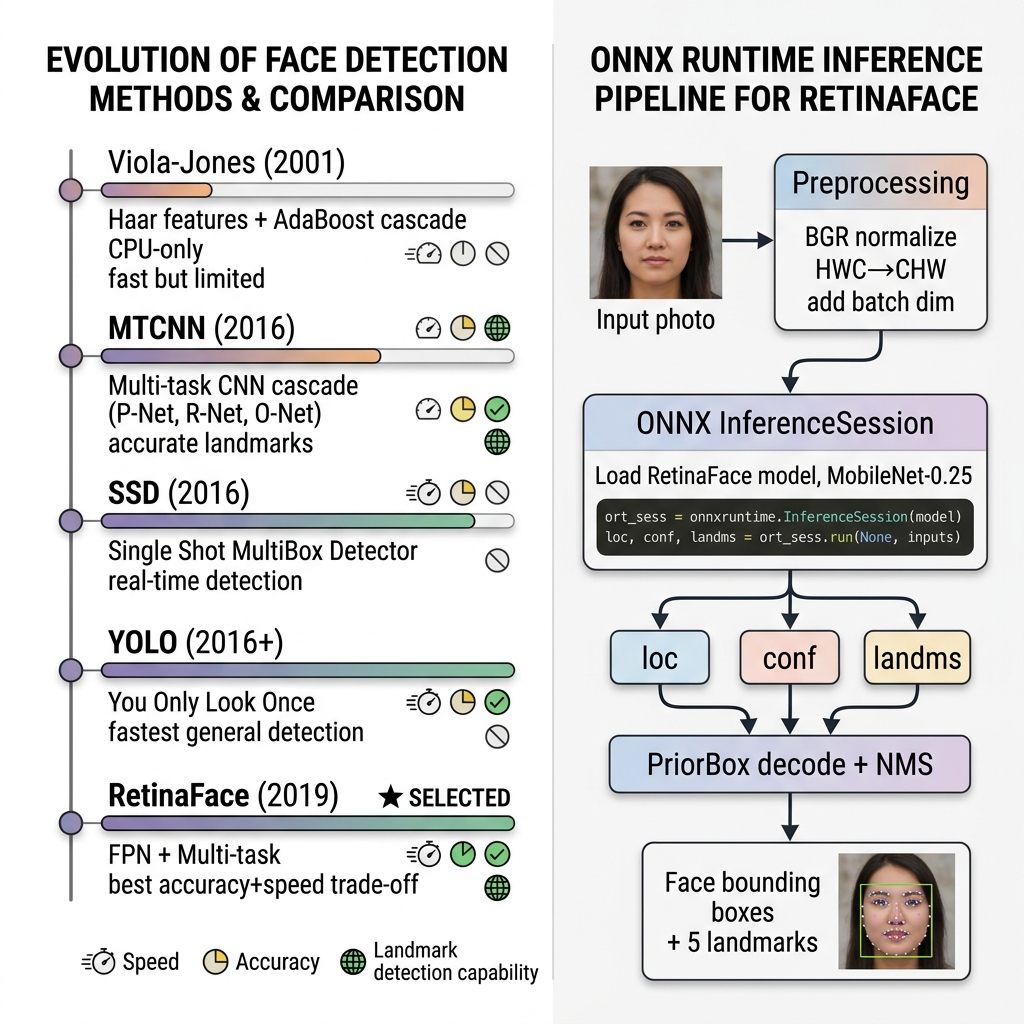
\includegraphics[width=0.85\textwidth]{figChap1/face_detection_pipeline.png}
    \caption{So sánh các phương pháp phát hiện khuôn mặt qua các thế hệ (trái) và pipeline suy luận ONNX Runtime của RetinaFace (phải)}
    \label{fig:face_detection_pipeline}
\end{figure}
    \noindent\textit{Chú thích:} RetinaFace được chọn vì cân bằng tốt nhất giữa tốc độ, độ chính xác và hỗ trợ facial landmarks đồng thời \cite{Deng2019RetinaFace, ONNX2019}


\begin{table}[H]
\caption{So sánh các phương pháp phát hiện khuôn mặt}
\label{tab:face_detection_comparison}
\centering
\begin{tabular}{|l|c|c|c|c|c|}
\hline
\textbf{Phương pháp} & \textbf{Năm} & \textbf{Landmark} & \textbf{Tốc độ} & \textbf{Mô hình} & \textbf{Backbone} \\
\hline
Viola-Jones & 2001 & Không & Nhanh & Cascade AdaBoost & Haar \\
\hline
MTCNN & 2016 & 5 pts & Trung bình & 3-stage CNN & 3× CNN nhỏ \\
\hline
SSD & 2016 & Không & Rất Nhanh & One-stage & VGG-16 \\
\hline
YOLOv5-face & 2021 & 5 pts & Rất Nhanh & One-stage & CSPNet \\
\hline
\textbf{RetinaFace} & \textbf{2019} & \textbf{5 pts} & \textbf{Nhanh} & \textbf{One-stage FPN} & \textbf{MobileNet-0.25} \\
\hline
\end{tabular}
\end{table}

\subsection{RetinaFace (Deng et al., 2019)}
\label{subsec:retinaface}

RetinaFace \cite{Deng2019RetinaFace} là phương pháp phát hiện khuôn mặt đơn giai đoạn
(single-shot) tiên tiến, được Deng et al. công bố tại CVPR 2020. Vì ba ưu điểm nổi bật: (1) phát hiện khuôn mặt đa
tỷ lệ từ rất nhỏ đến rất lớn; (2) đồng thời xuất bbox và 5 facial landmarks; (3) bản
MobileNet-0.25 cực kỳ nhẹ (~500KB) phù hợp triển khai thực tế.

\subsubsection{Kiến trúc: Feature Pyramid Network + Multi-task Learning}
\label{subsubsec:retinaface_architecture}

Kiến trúc RetinaFace kết hợp hai thành phần chính:

\textbf{(1) Backbone MobileNet-0.25:} Phiên bản thu nhỏ của MobileNet \cite{Howard2017MobileNet}
với hệ số chiều rộng 0.25, chỉ có khoảng 500K tham số. MobileNet sử dụng
\textit{Depthwise Separable Convolution} -- tách phép tích chập tiêu chuẩn thành tích chập
theo chiều sâu (depthwise) và tích chập điểm (pointwise $1\times1$) -- giảm tới 8--9 lần
số phép tính so với tích chập tiêu chuẩn \cite{Howard2017MobileNet}. Ba stage của backbone
xuất ra đặc trưng ở ba mức độ phân giải khác nhau (tương ứng stride 8, 16, 32), được chỉ
định trong \texttt{cfg\_mnet['return\_layers']} = \texttt{\{'stage1': 1, 'stage2': 2, 'stage3': 3\}}.

\textbf{(2) Feature Pyramid Network (FPN):} FPN \cite{Lin2017FPN} xây dựng một kim tự tháp
đặc trưng bằng cách kết hợp thông tin từ nhiều tầng của backbone qua hai đường:
\begin{itemize}
    \item \textit{Bottom-up pathway}: Đặc trưng từ backbone, độ phân giải giảm dần về phía đỉnh.
    \item \textit{Top-down pathway}: Đặc trưng từ tầng trên (ngữ nghĩa cao) được upsample và
    cộng phần tử (element-wise add) với đặc trưng từ tầng dưới (độ phân giải cao).
\end{itemize}
Kết quả là ba bản đồ đặc trưng $P_3, P_4, P_5$ có ngữ nghĩa phong phú ở mọi độ phân giải,
cho phép phát hiện khuôn mặt ở mọi kích thước trong một lần suy luận.

\textbf{(3) Multi-task Learning Heads:} Mỗi mức FPN có một Context Module (khối nhánh SSH --
Single Stage Headless Face Detector), xuất ra ba đầu ra đồng thời:

\begin{equation}
\label{eq:retinaface_loss}
\mathcal{L} = \mathcal{L}_{cls} + \lambda_1 \mathcal{L}_{box} + \lambda_2 \mathcal{L}_{pts}
\end{equation}
trong đó $\mathcal{L}_{cls}$ là binary cross-entropy loss phân loại khuôn mặt/nền
(face/background); $\mathcal{L}_{box}$ là smooth-$\ell_1$ loss hồi quy bounding box
(4 giá trị: $x_1, y_1, x_2, y_2$); và $\mathcal{L}_{pts}$ là smooth-$\ell_1$ loss hồi qui
5 facial landmarks (10 tọa độ: mắt trái, mắt phải, mũi, khóe miệng trái, khóe miệng phải)
\cite{Deng2019RetinaFace}. Trọng số $\lambda_1 = 2.0$ (xem \texttt{cfg\_mnet['loc\_weight']})
và $\lambda_2$ cân bằng giữa độ chính xác bbox và landmark.

\begin{figure}[H]
    \centering
    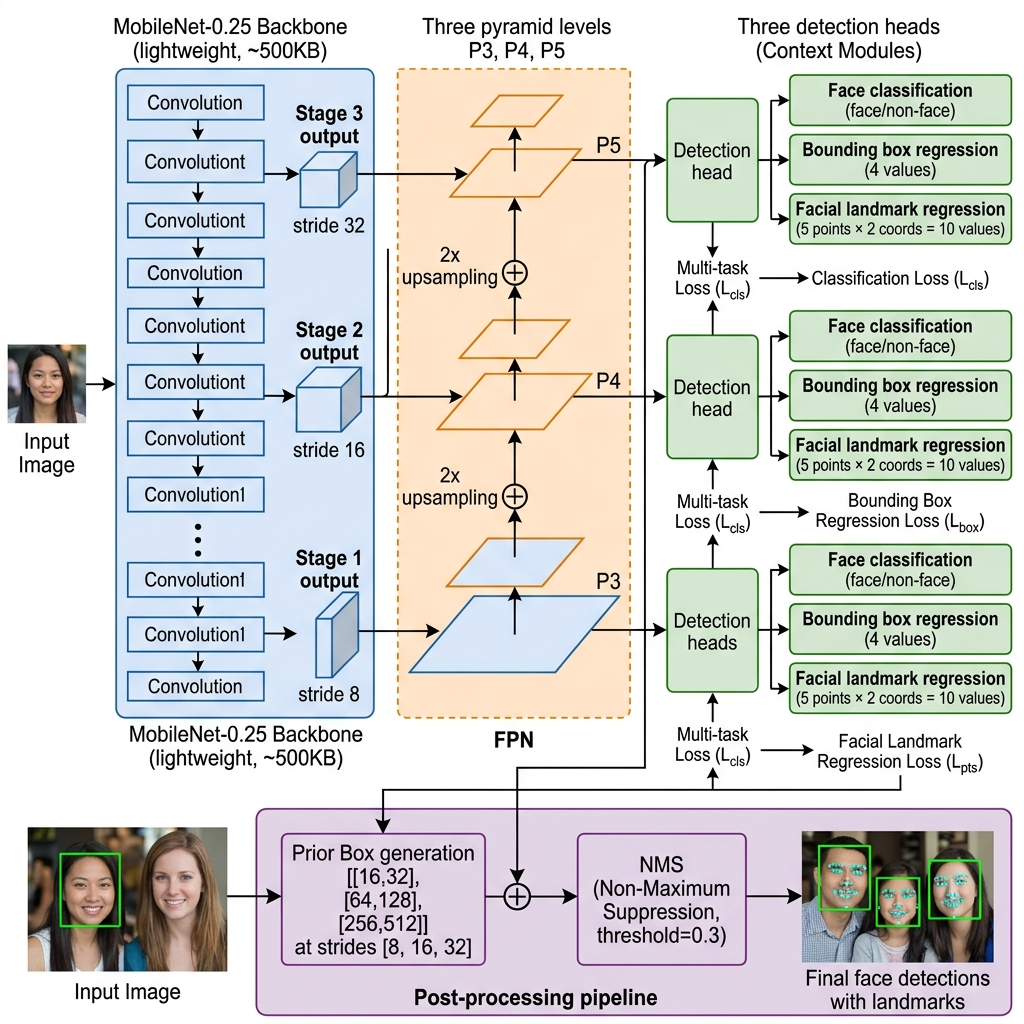
\includegraphics[width=\textwidth]{figChap1/retinaface_architecture.png}
    \caption{Kiến trúc RetinaFace với backbone MobileNet-0.25, Feature Pyramid Network (FPN) và ba detection head đa tác vụ}
    \label{fig:retinaface_architecture}
\end{figure}
    \noindent\textit{Chú thích:} Mỗi mức FPN phát hiện khuôn mặt ở một tỷ lệ khác nhau, đầu ra gồm bbox và 5 facial landmarks. Pipeline hậu xử lý bao gồm Prior Box decode và NMS \cite{Deng2019RetinaFace, Lin2017FPN}


\subsubsection{Anchor Boxes và Prior Box Generation}
\label{subsubsec:anchor_prior_box}

RetinaFace sử dụng cơ chế \textbf{anchor boxes} (hộp neo) để dự đoán vị trí khuôn mặt.
Cho mỗi ô (cell) trên bản đồ đặc trưng, mô hình dự đoán \textit{phần bù} (offset) so với
các anchor box được định nghĩa trước (prior boxes). Cấu hình anchor trong \texttt{cfg\_mnet}
(\texttt{retinaface\_/config.py}) như sau:

\begin{equation}
\label{eq:anchor_config}
\texttt{min\_sizes} = [\underbrace{[16, 32]}_{\text{stride}=8}, \underbrace{[64, 128]}_{\text{stride}=16}, \underbrace{[256, 512]}_{\text{stride}=32}]
\end{equation}

Tại mỗi mức đặc trưng với stride $s$, \textbf{Prior Box} (hộp neo trước) được tạo ra cho
từng ô lưới $(i, j)$ với tâm anchor:
\begin{equation}
\label{eq:prior_box}
c_x = \frac{(j + 0.5) \cdot s}{W}, \quad c_y = \frac{(i + 0.5) \cdot s}{H}
\end{equation}
trong đó $W, H$ là chiều rộng và cao của ảnh đầu vào ($640 \times 640$ theo \texttt{cfg\_mnet['image\_size']}). Với hai kích thước anchor tại mỗi mức, tổng số prior boxes cho
ảnh $640\times640$ là:
$(80^2 + 40^2 + 20^2) \times 2 = (6400 + 1600 + 400) \times 2 = 16800$ anchors.

\begin{figure}[H]
    \centering
    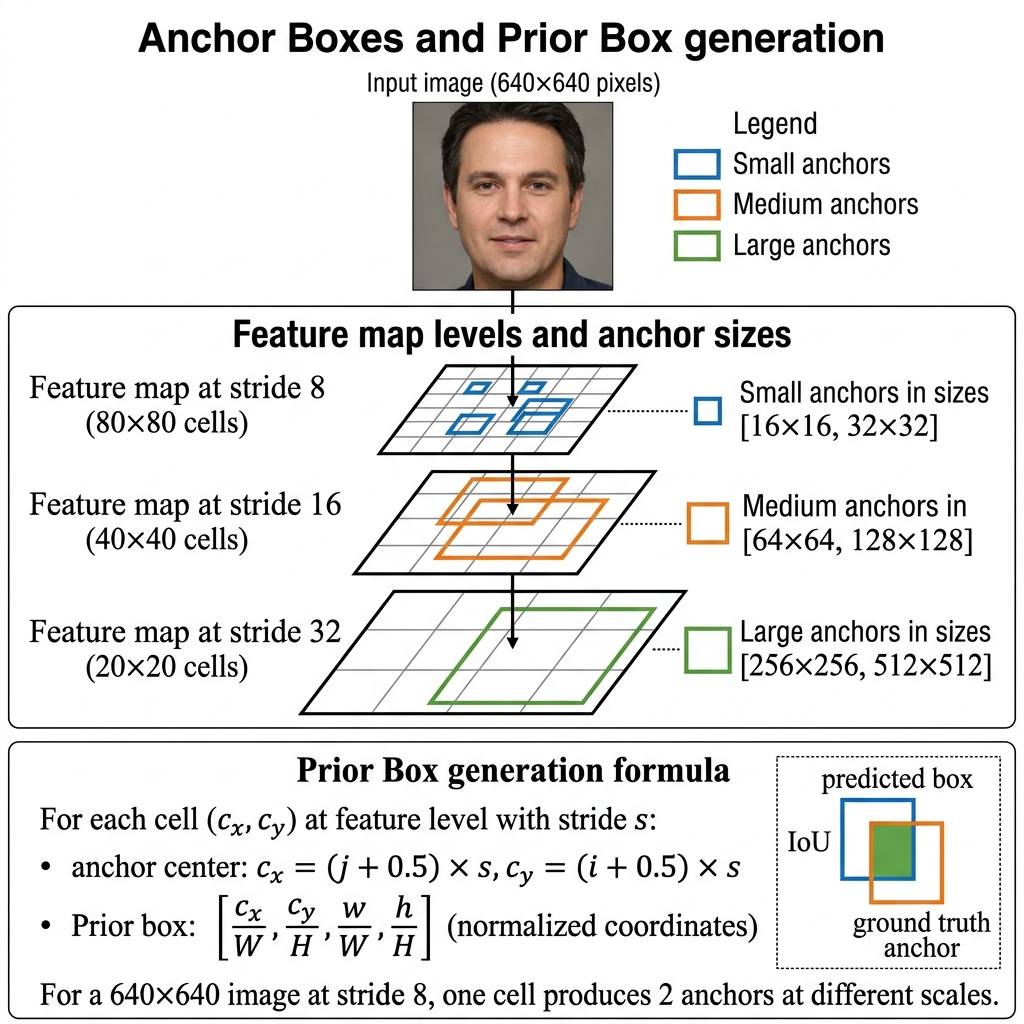
\includegraphics[width=0.92\textwidth]{figChap1/anchor_prior_box.png}
    \caption{Minh họa cơ chế Anchor Boxes trong RetinaFace}
    \label{fig:anchor_prior_box}
\end{figure}
    \noindent\textit{Chú thích:} Ba mức đặc trưng ứng với ba scale anchor khác nhau: anchors nhỏ $[16,32]$ tại stride 8 phát hiện khuôn mặt nhỏ; anchors trung $[64,128]$ tại stride 16 cho khuôn mặt trung bình; anchors lớn $[256,512]$ tại stride 32 cho khuôn mặt lớn chiếm phần lớn ảnh \cite{Deng2019RetinaFace}


\textbf{Non-Maximum Suppression (NMS):} Sau khi giải mã các prior boxes và lọc theo ngưỡng
confidence (\texttt{confidence\_threshold=0.8}), thuật toán NMS loại bỏ các hộp bounding box
trùng lặp. NMS giữ lại hộp tốt nhất và loại bỏ mọi hộp có IoU (Intersection over Union) với
hộp đó vượt quá ngưỡng \texttt{nms\_threshold=0.3}. Trong cài đặt \texttt{face\_det.py},
hàm \texttt{py\_cpu\_nms(dets, nms\_threshold)} thực hiện NMS theo thuật toán greedy:
\begin{enumerate}
    \item Sắp xếp các hộp theo điểm tin cậy (confidence score) giảm dần.
    \item Giữ hộp có điểm cao nhất.
    \item Loại bỏ mọi hộp có IoU $> 0.3$ với hộp vừa giữ.
    \item Lặp lại với hộp tiếp theo trong danh sách còn lại.
\end{enumerate}

\subsection{Suy luận với ONNX Runtime}
\label{subsec:onnx_inference}

Mô hình RetinaFace được lưu dưới dạng \textbf{ONNX} (Open Neural
Network Exchange) -- định dạng trung gian cho phép triển khai mô hình học sâu độc lập
với framework huấn luyện (TensorFlow, PyTorch) \cite{ONNX2019}. ONNX Runtime là bộ suy
luận tối ưu hóa cao hiệu năng cho định dạng ONNX, hỗ trợ nhiều nhà cung cấp tăng tốc
phần cứng (CPU, GPU, TensorRT...).

Các dòng 20--22 của \texttt{face\_det.py} khởi tạo phiên ONNX Runtime:
\begin{verbatim}
import onnxruntime                                            # L20

ort_sess_options = onnxruntime.SessionOptions()              # L21
ort_sess_options.intra_op_num_threads = int(               
    os.environ.get('ort_intra_op_num_threads', 0))

torch_mtcnn = onnxruntime.InferenceSession(                 # L22
    AES_de(assets_bin.faceDet, ...),
    sess_options=ort_sess_options)
\end{verbatim}

Đáng lưu ý: mặc dù biến được đặt tên là \texttt{torch\_mtcnn} (di sản lịch sử từ phiên
bản trước), mô hình thực tế được nạp là \textbf{RetinaFace MobileNet-0.25} được mã hóa AES
lưu trong \texttt{assets\_bin.faceDet}. Cấu hình \texttt{cfg = cfg\_mnet} tại dòng 28 xác
nhận điều này.

Quy trình suy luận đầy đủ trong hàm \texttt{detect\_face()} (\texttt{face\_det.py}):

\begin{enumerate}
    \item \textbf{Tiền xử lý ảnh:} Trừ giá trị trung bình màu sắc ImageNet
    $(123, 117, 104)$, chuyển đổi từ HWC sang CHW, thêm chiều batch.
    \item \textbf{Suy luận ONNX:} \texttt{ort\_outs = torch\_mtcnn.run(None, ort\_inputs)}
    trả về ba tensor: \texttt{loc} (vị trí bbox), \texttt{conf} (xác suất), \texttt{landms}
    (tọa độ landmarks).
    \item \textbf{Giải mã Prior Box:}
    \texttt{boxes = decode(loc, prior\_data, cfg['variance'])} chuyển offset về tọa độ
    tuyệt đối dùng phương sai \texttt{[0.1, 0.2]}.
    \item \textbf{Lọc và NMS:} Giữ các bbox có confidence $> 0.8$, áp dụng NMS với
    ngưỡng IoU $0.3$, giữ tối đa \texttt{keep\_top\_k=5} khuôn mặt.
    \item \textbf{Mở rộng vùng khuôn mặt:} Hàm \texttt{margin\_face()} mở rộng bbox
    thêm 50\% mỗi chiều (margin=0.5) để đảm bảo khuôn mặt đầy đủ cho Generator.
\end{enumerate}

\begin{table}[H]
\caption{Tham số cấu hình RetinaFace MobileNet-0.25}
\label{tab:retinaface_config}
\centering
\begin{tabular}{|l|p{4cm}|l|}
\hline
\textbf{Tham số} & \textbf{Giá trị} & \textbf{Ý nghĩa} \\
\hline
\texttt{name} & \texttt{'mobilenet0.25'} & Backbone nhẹ 0.25$\times$ chiều rộng \\
\hline
\texttt{min\_sizes} & \texttt{[[16,32], [64,128], [256,512]]} & Kích thước anchor 3 mức FPN \\
\hline
\texttt{steps} & \texttt{[8, 16, 32]} & Stride 3 mức feature map \\
\hline
\texttt{variance} & \texttt{[0.1, 0.2]} & Hệ số giải mã bbox / landmark \\
\hline
\texttt{loc\_weight} & \texttt{2.0} & Trọng số loss bbox trong $\mathcal{L}$ \\
\hline
\texttt{image\_size} & \texttt{640} & Kích thước ảnh đầu vào max \\
\hline
\texttt{in\_channel} & \texttt{32} & Số kênh vào FPN \\
\hline
\texttt{out\_channel} & \texttt{64} & Số kênh ra FPN \\
\hline
\texttt{confidence\_threshold} & \texttt{0.8} & Ngưỡng lọc khuôn mặt \\
\hline
\texttt{nms\_threshold} & \texttt{0.3} & Ngưỡng NMS \\
\hline
\end{tabular}
\end{table}

Việc sử dụng ONNX Runtime cho phép triển khai mô hình phát hiện khuôn mặt
mà không cần cài đặt PyTorch hay TensorFlow, giảm đáng kể kích thước phụ thuộc của ứng dụng
\cite{ONNX2019}. Kết hợp với backbone MobileNet-0.25 siêu nhẹ \cite{Howard2017MobileNet},
toàn bộ bộ phát hiện khuôn mặt đạt tốc độ thời gian thực trên CPU thông thường, là nền tảng
cho trải nghiệm người dùng mượt mà trong ứng dụng chuyển phong cách anime tương tác.


\section{Lọc Ảnh và Tiền Xử Lý}
\label{sec:image_preprocessing}

Chất lượng dữ liệu huấn luyện đóng vai trò quyết định trong kết quả của các mô hình GAN
cho phong cách anime. AnimeGANv3 áp dụng một chuỗi kỹ thuật tiền xử lý ảnh đặc thù để
biến đổi ảnh anime thô thành các tập con dữ liệu tham chiếu có đặc tính kỹ thuật phù hợp
với từng thành phần hàm mất mát. Cụ thể, bộ dữ liệu huấn luyện bao gồm: (1) ảnh anime gốc
$a$, (2) phiên bản đã làm mịn cạnh $e$ (dùng cho \textit{edge loss}), và (3) ảnh được
phân vùng và làm mượt $s$ (dùng cho \textit{region smoothing loss}) \cite{Liu2024}.

\begin{figure}[H]
    \centering
    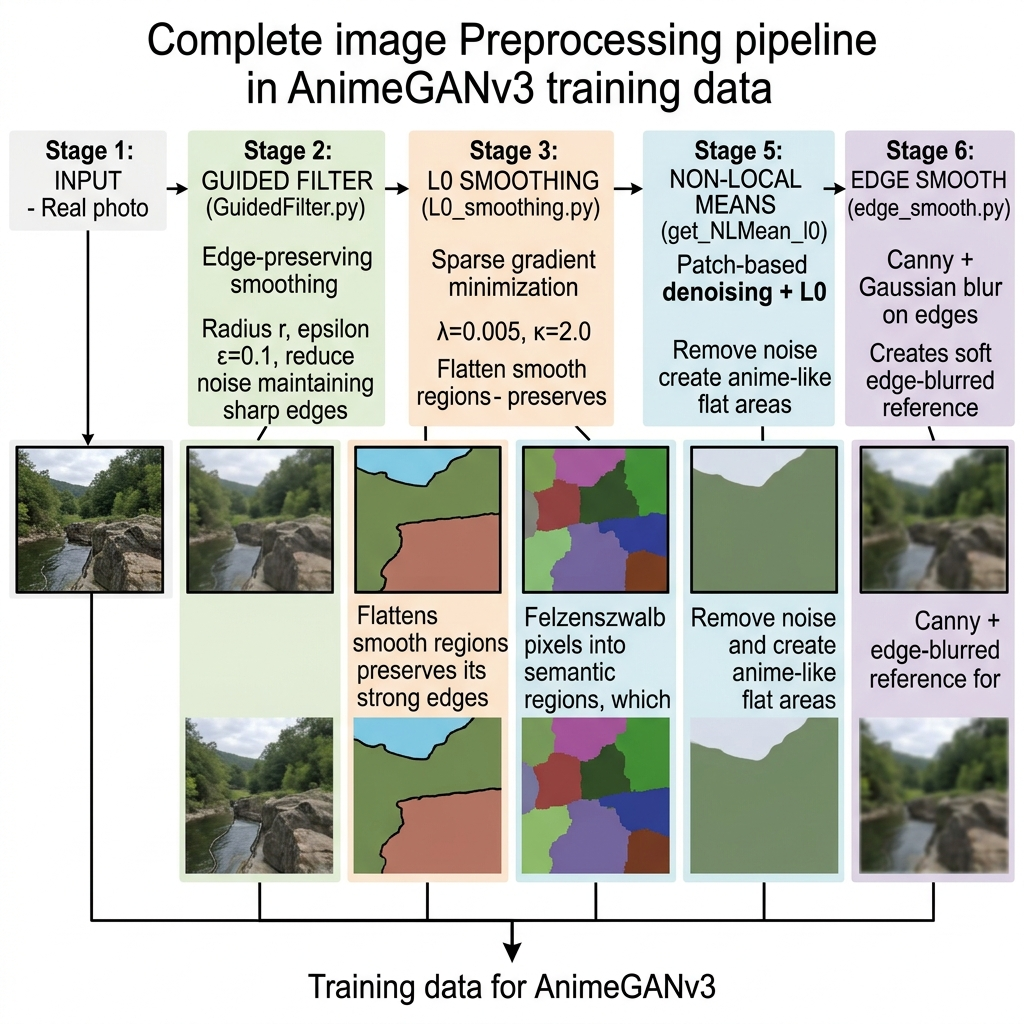
\includegraphics[width=0.85\textwidth]{figChap1/image_preprocessing_pipeline.png}
    \caption{Pipeline tiền xử lý dữ liệu huấn luyện của AnimeGANv3}
    \label{fig:image_preprocessing_pipeline}
\end{figure}
    \noindent\textit{Chú thích:} Từ ảnh anime gốc, các kỹ thuật Guided Filter, L0 Smoothing, Superpixel Segmentation, Non-Local Means Denoising và Edge Smoothing được áp dụng tuần tự để tạo ra các tập dữ liệu tham chiếu phục vụ các hàm mất mát khác nhau trong quá trình huấn luyện \cite{Liu2024, He2013GuidedFilter, Xu2011L0}


\subsection{Guided Filter}
\label{subsec:guided_filter}

\textbf{Guided Image Filtering} \cite{He2013GuidedFilter} là kỹ thuật lọc ảnh bảo toàn cạnh
(edge-preserving filter) do He et al. đề xuất tại IEEE TPAMI 2013. Khác với bộ lọc Gaussian
làm mờ đồng đều cả cạnh sắc lẫn vùng phẳng, Guided Filter sử dụng một \textit{ảnh hướng dẫn}
(guidance image) $I$ để kiểm soát mức độ làm mịn, bảo toàn các cạnh mạnh trong khi vẫn
loại bỏ nhiễu và chi tiết nhỏ trong vùng màu đồng nhất \cite{He2013GuidedFilter}.

\textbf{Mô hình toán học:} Guided Filter giả định rằng đầu ra $q$ là biến đổi tuyến tính
cục bộ của ảnh hướng dẫn $I$ trong mỗi cửa sổ $\omega_k$ bán kính $r$:
\begin{equation}
\label{eq:guided_filter_model}
q_i = a_k I_i + b_k, \quad \forall i \in \omega_k
\end{equation}
trong đó các hệ số $(a_k, b_k)$ được ước tính từ ảnh đầu vào $p$ (ảnh cần lọc) bằng cách
tối thiểu hóa sai số:
\begin{equation}
\label{eq:guided_filter_minimize}
\min_{a_k, b_k} \sum_{i \in \omega_k} \left[(a_k I_i + b_k - p_i)^2 + \varepsilon a_k^2\right]
\end{equation}
Nghiệm tối ưu cho hệ số $a_k$ (thể hiện độ nhạy cạnh) và $b_k$ (độ dịch chuyển) là:
\begin{equation}
\label{eq:guided_filter_coeff}
a_k = \frac{\overline{Ip}_k - \bar{I}_k\bar{p}_k}{\sigma^2_{I,k} + \varepsilon}, \qquad
b_k = \bar{p}_k - a_k \bar{I}_k
\end{equation}
trong đó $\sigma^2_{I,k}$ là phương sai của $I$ trong $\omega_k$; $\varepsilon$ là tham số
điều chuẩn (regularization) ngăn chặn $a_k$ quá lớn \cite{He2013GuidedFilter}. Khi $I = p$
(self-guided filter), $a_k$ lớn tại cạnh (phương sai cao) và nhỏ tại vùng phẳng (phương sai
thấp), dẫn đến cạnh được bảo toàn và vùng phẳng được làm mịn.

\begin{figure}[H]
    \centering
    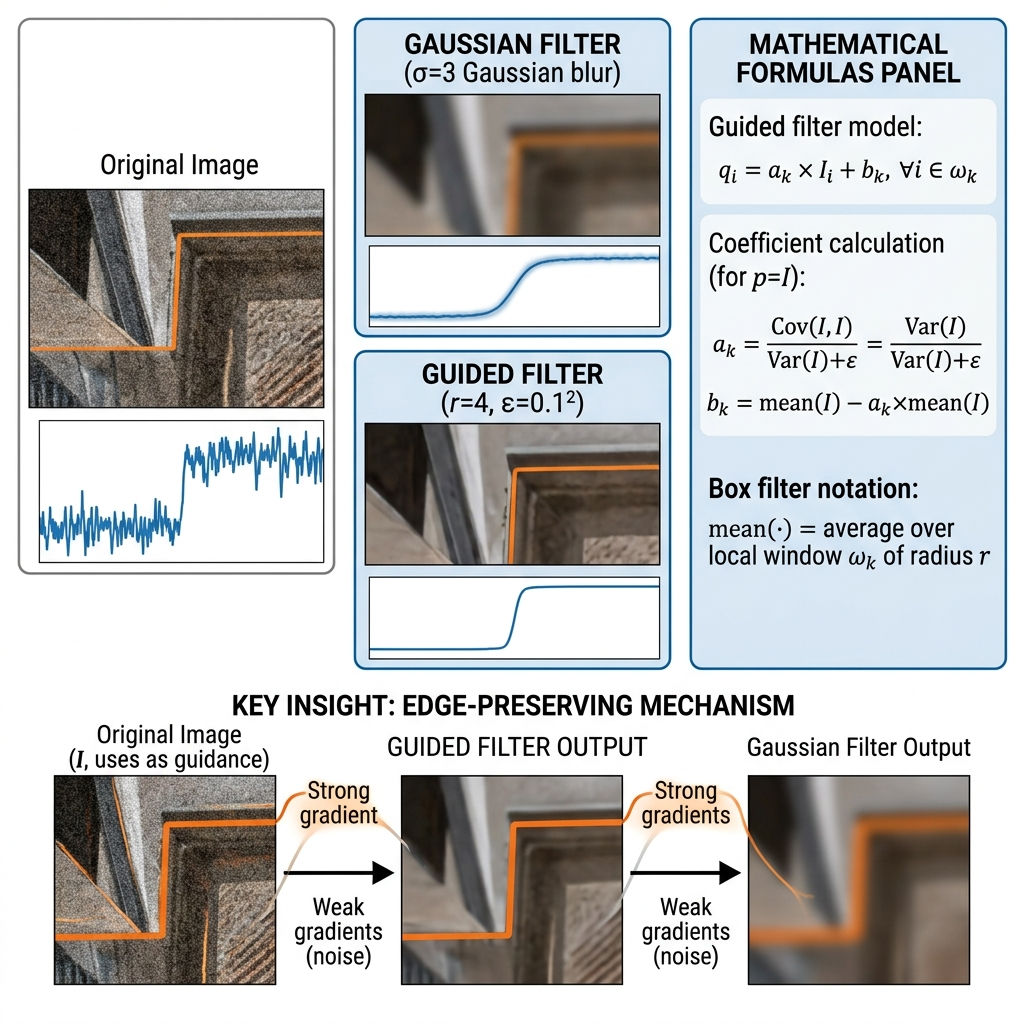
\includegraphics[width=0.85\textwidth]{figChap1/guided_filter_vs_gaussian.png}
    \caption{So sánh Guided Filter và Gaussian Filter}
    \label{fig:guided_filter_vs_gaussian}
\end{figure}
    \noindent\textit{Chú thích:} Gaussian Filter làm mờ không phân biệt cạnh và vùng phẳng. Guided Filter bảo toàn cạnh sắc bằng cách điều chỉnh hệ số $a_k$ theo phương sai cục bộ, chỉ làm mịn những vùng đồng nhất (phương sai thấp) \cite{He2013GuidedFilter}


\textbf{Cài đặt trong AnimeGANv3} (\texttt{GuidedFilter.py}): Hàm \texttt{guided\_filter(x, y, r, eps)}
sử dụng \textit{box filter} được tính hiệu quả qua tổng tích lũy (cumulative sum --
\texttt{tf.cumsum}) thay vì tích chập trực tiếp, giảm độ phức tạp từ $O(r^2)$ xuống $O(1)$
bất kể bán kính $r$. Tham số điển hình: $r \in \{2,3,4,5\}$, $\varepsilon \in \{0.01, 0.04, 0.16\}$.

\subsection{L0 Smoothing}
\label{subsec:l0_smoothing}

\textbf{L0 Gradient Minimization} \cite{Xu2011L0} là kỹ thuật làm mịn ảnh cực đơn giản hóa:
thay vì giảm \textit{độ lớn} gradient (như $\ell_1, \ell_2$), L0 Smoothing tối thiểu hóa
\textit{số lượng} gradient khác không, tạo ra ảnh với rất ít vùng biến đổi gradient nhưng
các cạnh còn lại thì cực kỳ sắc nét \cite{Xu2011L0}. Đây là đặc tính lý tưởng mô phỏng
phong cách tranh anime: màu phẳng trong vùng lớn, cạnh rõ ràng và mạnh.

\textbf{Hàm mục tiêu L0:}
\begin{equation}
\label{eq:l0_objective}
\min_S \left\{ \sum_{p}(S_p - I_p)^2 + \lambda \cdot \#\{p \mid |\partial_x S_p| + |\partial_y S_p| \neq 0\} \right\}
\end{equation}
trong đó $I$ là ảnh gốc, $S$ là ảnh đầu ra cần tìm; số hạng đầu là fidelity term đảm bảo
$S$ gần với $I$; số hạng sau đếm số pixel có gradient khác không (\textit{L0 pseudo-norm});
$\lambda$ điều chỉnh mức độ làm mịn \cite{Xu2011L0}.

\textbf{Giải thuật Half-Quadratic Splitting} (\texttt{L0\_smoothing.py}):
Do bài toán $\ell_0$ không lồi và không khả vi, Xu et al. \cite{Xu2011L0} đề xuất xấp xỉ
bằng cách thêm biến phụ $(h, v)$ đại diện cho gradient và giải xen kẽ hai bài toán con
qua vòng lặp với $\beta = \lambda_0 \cdot \kappa$ tăng dần ($\kappa = 2$):
\begin{enumerate}
    \item \textbf{$h,v$-subproblem (Thresholding):} Cập nhật gradient phụ qua ngưỡng cứng:
    nếu $h_p^2 + v_p^2 < \lambda/\beta$ thì đặt $(h_p, v_p) = 0$ (buộc vùng phẳng).
    \item \textbf{$S$-subproblem (FFT):} Cập nhật $S$ trong miền tần số (Fourier domain)
    bằng phép chia ma trận phổ, tính $O(N\log N)$ qua FFT thay vì $O(N^2)$.
\end{enumerate}

Trong AnimeGANv3, hàm \texttt{L0Smoothing(Im, lamda=2e-2, kappa=2.0)} được gọi để xử lý
ảnh anime trước khi đưa vào huấn luyện, tạo ra ảnh $a'$ với vùng phẳng rõ ràng phục vụ
\textit{Region Smoothing Loss}.

\begin{table}[H]
\caption{So sánh các kỹ thuật làm mịn ảnh trong AnimeGANv3}
\label{tab:smoothing_comparison}
\centering
\begin{tabular}{|l|p{3cm}|p{3cm}|p{3.5cm}|}
\hline
\textbf{Kỹ thuật} & \textbf{Bảo toàn cạnh} & \textbf{Kết quả} & \textbf{Ứng dụng} \\
\hline
Gaussian Filter & Thấp (cạnh bị mờ) & Toàn ảnh mờ đồng đều & Tiền xử lý chung \\
\hline
Guided Filter & Cao (bảo toàn nghiêm ngặt) & Mịn + cạnh sắc & Làm mịn thích ứng \\
\hline
L0 Smoothing & Rất cao (cạnh nhọn) & Màu phẳng + cạnh cứng & Phong cách anime\\
\hline
NLM Denoising & Cao (dựa trên patch) & Khử nhiễu không gian & Ảnh có noise \\
\hline
\end{tabular}
\end{table}

\subsection{Superpixel Segmentation (Felzenszwalb)}
\label{subsec:superpixel}

Phân vùng siêu điểm ảnh (\textbf{Superpixel Segmentation}) nhóm các pixel lân cận
có màu sắc và kết cấu tương đồng thành các vùng (superpixels) đồng nhất hơn. Trong
AnimeGANv3, phân vùng superpixel được thực hiện qua hàm \texttt{get\_seg()} sử dụng
thuật toán của \textbf{Felzenszwalb và Huttenlocher} \cite{Felzenszwalb2004} --
một trong những phương pháp phân vùng đồ thị đầu tiên đạt độ phức tạp gần tuyến tính.

\textbf{Nguyên lý Felzenszwalb Segmentation:} Ảnh được biểu diễn như một đồ thị vô hướng
$G = (V, E)$ trong đó mỗi pixel là một đỉnh và các cạnh $(u,v) \in E$ kết nối các pixel
lân cận với trọng số $w(u,v)$ = sự khác biệt cường độ. Thuật toán định nghĩa tiêu chí
hợp nhất vùng dựa trên \textit{Minimum Spanning Tree} (MST): hai vùng $C_1, C_2$ nên
được hợp nhất nếu \cite{Felzenszwalb2004}:
\begin{equation}
\label{eq:felzenszwalb}
D(C_1, C_2) < \mathrm{MInt}(C_1, C_2)
\end{equation}
trong đó $D(C_1, C_2) = \min_{v_i \in C_1, v_j \in C_2} w(v_i, v_j)$ là cạnh nhỏ nhất
giữa hai vùng; và $\mathrm{MInt}(C_i) = \max_{(u,v) \in \mathrm{MST}(C_i)} w(u,v) + k/|C_i|$
là ``độ nhất quán nội bộ'' của vùng ($k$ điều chỉnh độ thô của phân vùng).

\textbf{Ứng dụng trong AnimeGANv3:} Sau khi phân vùng, mỗi superpixel được tô màu bằng
giá trị trung bình (mean color) của các pixel thuộc vùng đó, tạo ra ảnh có vùng màu phẳng
hoàn toàn -- đặc điểm đặc trưng của tranh anime. Kết quả này được sử dụng như tín hiệu
tham chiếu trong \textit{Region Smoothing Loss} của AnimeGANv3.

\subsection{Non-Local Means Denoising}
\label{subsec:nlm_denoising}

\textbf{Non-Local Means} (NLM) \cite{Buades2005NLM} là thuật toán khử nhiễu phi cục bộ
do Buades et al. giới thiệu tại CVPR 2005, vượt trội hơn các phương pháp cục bộ như
Gaussian hay Median filter nhờ khai thác tính lặp lại cấu trúc (self-similarity) trong ảnh.

\textbf{Nguyên lý phi cục bộ:} Giá trị được khử nhiễu tại pixel $\mathbf{x}$ được tính
là trung bình có trọng số của \textit{tất cả} pixel trong ảnh, với trọng số dựa trên sự
tương đồng \textit{patch} (vùng nhỏ xung quanh pixel):
\begin{equation}
\label{eq:nlm}
\mathrm{NL}[u](\mathbf{x}) = \frac{1}{C(\mathbf{x})} \int_\Omega \exp\!\left(-\frac{\|B(\mathbf{x}) - B(\mathbf{y})\|^2_{2,a}}{h^2}\right) u(\mathbf{y}) \, d\mathbf{y}
\end{equation}
trong đó $B(\mathbf{x})$ là patch xung quanh $\mathbf{x}$; $h$ là tham số lọc điều chỉnh
mức độ suy giảm; và $C(\mathbf{x})$ là hằng số chuẩn hóa \cite{Buades2005NLM}. Khi hai
patch $B(\mathbf{x})$ và $B(\mathbf{y})$ rất giống nhau, trọng số gần 1 (pixel ảnh hưởng
mạnh); khi khác nhau nhiều, trọng số tiệm cận 0.

\textbf{Hàm \texttt{get\_NLMean\_l0()} trong AnimeGANv3:} Kết hợp NLM Denoising với
L0 Smoothing theo quy trình: (1) áp dụng NLM để loại bỏ nhiễu hạt (grain noise) và
nhiễu nén JPEG đặc trưng trong ảnh anime scan; (2) áp dụng L0 Smoothing để tạo vùng
màu phẳng. Quy trình kép này giúp tạo ra tập dữ liệu tham chiếu phong cách ``anime thuần''
không nhiễu, không kết cấu thực, mà có màu sắc chuẩn và cạnh rõ.

\subsection{Edge Smoothing}
\label{subsec:edge_smoothing}

\textbf{Edge Smoothing} (\texttt{edge\_smooth.py}) là bước tiền xử lý được kế thừa từ
CartoonGAN \cite{Chen2018CartoonGAN} (taki0112/CartoonGAN-TensorFlow), tạo ra tập ảnh
$e$ có đặc điểm: cạnh mạnh được giữ nguyên nhưng vùng lân cận cạnh được làm mịn nhẹ
bằng Gaussian. Mục tiêu là tạo ra dữ liệu huấn luyện có ``cạnh mềm'' để hướng dẫn
Generator học tạo ra nét viền anime tự nhiên, không quá cứng.

\textbf{Quy trình trong \texttt{make\_edge\_smooth()} (\texttt{edge\_smooth.py}):}
\begin{enumerate}
    \item \textbf{Phát hiện cạnh Canny:} \texttt{edges = cv2.Canny(gray\_img, 100, 200)}
    -- tìm cạnh mạnh trong ảnh xám với ngưỡng thấp 100 và ngưỡng cao 200.
    \item \textbf{Giãn nở cạnh (Dilation):} \texttt{dilation = cv2.dilate(edges, kernel)}
    -- kernel $5 \times 5$, mở rộng vùng cạnh để bao phủ vùng lân cận.
    \item \textbf{Làm mịn Gaussian có chọn lọc:} \textit{Chỉ} tại các pixel thuộc vùng cạnh
    đã giãn nở (\texttt{idx = np.where(dilation != 0)}), thực hiện tích chập với kernel
    Gaussian $5 \times 5$: $q_p = \sum_{(i,j)} G_{\sigma}(i,j) \cdot I_{p+(i,j)}$.
\end{enumerate}

Phương pháp này tạo ra ảnh $e$ với đặc điểm quan trọng: vùng \textit{không phải cạnh} giữ
nguyên pixel gốc (không bị mờ), chỉ vùng \textit{gần cạnh} được làm mịn nhẹ. Điều này
tạo ``vùng đệm'' Gaussian xung quanh các đường nét anime, giúp Generator trong quá trình
huấn luyện tổng quát hóa sang các phong cách cạnh khác nhau, thay vì chỉ học cạnh cứng.

\textbf{Công thức hàm mất mát Edge trong AnimeGANv3:}

Tập ảnh $e$ (edge-smoothed) được dùng trong thành phần \textit{Edge Loss} hoặc phân biệt
bởi Discriminator riêng, buộc Generator sinh ra ảnh anime có phong cách nét viền phù hợp:
\begin{equation}
\label{eq:edge_loss}
\mathcal{L}_{edge} = \mathbb{E}_{e \sim \mathcal{E}}\left[\log(1 - D(e))\right]
\end{equation}
trong đó $\mathcal{E}$ là phân phối của tập ảnh edge-smoothed và $D$ là Discriminator
\cite{Chen2018CartoonGAN, Liu2024}.

\begin{table}[H]
\caption{Tóm tắt các kỹ thuật tiền xử lý dữ liệu trong AnimeGANv3}
\label{tab:preprocessing_summary}
\centering
\begin{tabular}{|p{3cm}|p{3.6cm}|p{2.9cm}|p{3.5cm}|}
\hline
\textbf{Kỹ thuật} & \textbf{File tham chiếu} & \textbf{Đầu ra} & \textbf{Dùng trong Loss} \\
\hline
Guided Filter & \texttt{GuidedFilter.py} & Ảnh mịn, cạnh sắc & Tiền xử lý chung \\
\hline
L0 Smoothing & \texttt{L0\_smoothing.py} & Màu phẳng, cạnh mạnh & Region Smoothing Loss \\
\hline
Superpixel (Felzenszwalb) & \texttt{get\_seg()} & Vùng màu đồng nhất & Region Smoothing Loss \\
\hline
Non-Local Means & \texttt{get\_NLMean\_l0()} & Khử nhiễu + phẳng màu & Region Smoothing Loss \\
\hline
Edge Smoothing & \texttt{edge\_smooth.py} & Cạnh mờ nhẹ & Edge / Discriminator Loss \\
\hline
\end{tabular}
\end{table}

Sự kết hợp có chủ đích của năm kỹ thuật tiền xử lý này phản ánh thấu hiểu sâu sắc về
đặc điểm hình ảnh học (visual characteristics) của phong cách anime: màu phẳng theo vùng,
cạnh viền rõ ràng và nhất quán, không nhiễu, và phân bố màu sắc khác biệt rõ ràng so với
ảnh chụp thực tế. Chính nhờ thiết kế pipeline huấn luyện chuyên biệt này mà AnimeGANv3
đạt chất lượng chuyển đổi phong cách anime vượt trội so với các phương pháp trước
\cite{Liu2024, He2013GuidedFilter, Xu2011L0, Felzenszwalb2004, Buades2005NLM, Chen2018CartoonGAN}.





















